\chapter{LANDASAN TEORI}

Pada bab ini akan dibahas mengenai konsep, teori, dan referensi yang menjadi
dasar dalam melakukan analisis suatu metode statistik. Konsep dasar yang
dibahas pada bab ini adalah ...

\section{Aljabar Matriks}
Aljabar linear merupakan salah satu fondasi matematis terpenting dalam
statistika, ekonometrika, serta pembelajaran mesin. Banyak metode regresi
spasial maupun spasial-temporal, termasuk model berbasis jaringan saraf graf
atau \emph{graph neural networks} (GNN), dapat diformulasikan dalam kerangka operasi matriks. Oleh karena itu, pemahaman yang kuat mengenai struktur vektor dan matriks serta sifat-sifat aljabarnya diperlukan sebelum membahas metode regresi terboboti geografis.

\subsection{Ruang Vektor dan Matriks}
Pembahasan aljabar linear umumnya berangkat dari konsep lapangan atau
\emph{field} sebagai struktur aljabar dasar tempat bilangan berlaku. Dari
lapangan, dibangun ruang vektor, kemudian matriks sebagai representasi
transformasi linear, dan tensor sebagai generalisasi multidimensi.

\begin{definisi}[\textbf{Lapangan, \citep{lang_serge}}]
    Misalkan $K$ adalah subhimpunan dari bilangan kompleks $\mathbb{C}$, $K$ disebut sebagai lapangan apabila memenuhi kondisi berikut.
    \begin{enumerate}[label=(\alph*)]
        \item Apabila $x,y$ adalah elemen dari $K$, maka $x+y$ dan $xy$ juga merupakan elemen
              dari $K$.
        \item Apabila $x \in K$, maka $-x$ juga merupakan elemen dari $K$. Lebih lanjut, jika
              $x\ne0$, maka $x^{-1}$ merupakan elemen dari $K$.
        \item 0 dan 1 merupakan elemen dari $K$.
    \end{enumerate}
\end{definisi}

\noindent Berdasarkan definisi di atas, dapat diperhatikan bahwa $\mathbb{R}$ dan $\mathbb{C}$ merupakan lapangan.

\begin{contoh}
    Apabila dinotasikan $\mathbb{Q}$ sebagai himpunan bilangan rasional, yaitu
    \begin{equation}
        \mathbb{Q} = \left\{ \frac{m}{n} : m,n \in \mathbb{Z},\, n \neq 0 \right\},
    \end{equation}
    maka dapat dinyatakan bahwa $\mathbb{Q}$ membentuk suatu lapangan.
    Misalkan $\tfrac{a}{b}, \tfrac{c}{d} \in \mathbb{Q}$ dengan $a,b,c,d \in \mathbb{Z}$ dan $b,d \neq 0$.
    Jelas bahwa
    \begin{equation}
        \frac{a}{b} + \frac{c}{d} = \frac{ad + bc}{bd} \in \mathbb{Q},
    \end{equation}
    sehingga sifat tertutup terhadap penjumlahan, sebagai salah satu aksioma lapangan, terpenuhi.  Lebih lanjut, untuk setiap $\tfrac{a}{b} \in \mathbb{Q}$ berlaku pula bahwa $-\tfrac{a}{b} \in \mathbb{Q}$.
    Selain itu, jika $a \neq 0$, maka invers perkalian $\tfrac{a}{b}$ diberikan oleh
    \begin{equation}
        \left(\frac{a}{b}\right)^{-1} = \frac{b}{a} \in \mathbb{Q}.
    \end{equation}
    Dengan demikian, keberadaan invers aditif dan invers perkalian juga terjamin.  Akhirnya, apabila dipilih $\tfrac{a}{b} = \tfrac{0}{1}$ dan $\tfrac{a}{b} = \tfrac{1}{1}$, diperoleh bahwa elemen identitas penjumlahan $0$ dan identitas perkalian $1$ termasuk dalam $\mathbb{Q}$. Di sisi lain, dapat dengan mudah diperiksa bahwa $\mathbb{Z}$ bukan merupakan lapangan, karena apabila $n\in\mathbb{Z}$ dan $n\ne0$, jelas bahwa $n^{-1}\notin\mathbb{Z}$, kecuali untuk kasus $n=1$ atau $n=-1$.
\end{contoh}

Dalam ruang vektor dan matriks, dikenal juga istilah sublapangan. Apabila $K$
dan $L$ keduanya merupakan lapangan, serta dimisalkan bahwa $K\subseteq L$,
maka $K$ dapat disebut sebagai sublapangan atau \emph{subfield} dari $L$.
Elemen-elemen dari lapangan disebut sebagai bilangan atau skalar.
(\citealp{lang_serge})

\begin{definisi}[\textbf{Ruang Vektor, \citep{lang_serge}}]
    Suatu ruang vektor $V$ atas suatu lapangan $K$ adalah sebuah himpunan objek yang dapat dijumlahkan dan dikalikan dengan elemen-elemen dari $K$, sedemikian rupa sehingga hasil penjumlahan dua elemen dari $V$ merupakan elemen $V$ kembali, dan hasil perkalian  sebuah elemen $V$ dengan sebuah elemen dari $K$ juga merupakan elemen dari $V$.
    Selain itu, sifat-sifat berikut dipenuhi:
    \begin{enumerate}[label=(\alph*)]
        \item $\forall u, v, w \in V$ berlaku $(u+v)+w = u+(v+w)$.
        \item $\exists\, 0 \in V$ sedemikian sehingga $\forall u \in V$ berlaku $u + 0 = u$.
        \item $\forall u \in V$, $\exists -u \in V$ sedemikian sehingga $u + (-u) = 0$.
        \item $\forall u, v \in V$ berlaku $u+v = v+u$.
        \item $\forall c \in K$ dan $\forall u,v \in V$ berlaku $c\,(u+v) = cu + cv$.
        \item $\forall a,b \in K$ dan $\forall v \in V$ berlaku $(a+b)v = av + bv$.
        \item $\forall a,b \in K$ dan $\forall v \in V$ berlaku $(ab)v = a(bv)$.
        \item $\forall u \in V$ berlaku $1 \cdot u = u,$ dengan $1$ adalah elemen identitas pada $K$.
    \end{enumerate}
\end{definisi}

Dalam mendefinisikan ruang vektor, lapangan tempat ruang vektor berada harus
didefinisikan dengan spesifik, misalnya $\mathbb{C}^n$ merupakan ruang vektor
atas $\mathbb{C}$, tetapi $\mathbb{R}^n$ bukan ruang vektor atas $\mathbb{C}$.
$\mathbb{R}^n$ merupakan ruang vektor atas $\mathbb{R}$.

\begin{definisi}[\textbf{Ruang Matriks, \citep{lang_serge}}]
    Misalkan $K$ merupakan lapangan dan $m,n\ge1\in\mathbb{Z}$. Matriks adalah suatu larik atau \emph{array} dari bilangan-bilangan dalam $K$ yang dinotasikan sebagai
    $$
        \begin{pmatrix}
            a_{11} & a_{12} & \cdots & a_{1n} \\
            a_{21} & a_{22} & \cdots & a_{2n} \\
            \vdots & \vdots & \ddots & \vdots \\
            a_{m1} & a_{m2} & \cdots & a_{mn}
        \end{pmatrix}.
    $$
\end{definisi}
\noindent Notasi matriks pada definisi di atas dapat dipersingkat dengan menulis $(a_{ij}),\, i=1,2,\dots,m$ dan $j=1,2,\dots,n$. Matriks tersebut merupakan matriks $m \times n$ yang berarti bahwa matriks tersebut memiliki $m$-baris dan $n$-kolom. Sebagai contoh, kolom pertama dari matriks tersebut adalah
$$
    \begin{pmatrix}
        a_{11} \\ a_{21} \\ \vdots \\ a_{m1}
    \end{pmatrix}
$$
dan baris pertamanya adalah $(a_{11}, a_{12},\dots,a_{1n})$. Nilai $a_{ij}$ disebut sebagai komponen dari matriks.

Dua buah matriks dikatakan sama apabila keduanya memiliki ukuran yang sama dan
elemen-elemen pada posisi yang bersesuaian juga sama. Oleh karena itu, jika
$\*A = (a_{ij})$ dan $\*B = (b_{ij})$, maka $\*A = \*B$ apabila $a_{ij} =
    b_{ij}$, untuk seiap $i, j$.

\begin{definisi}[\textbf{Kebebasan Linear, \citep{lang_serge}}]
    Misalkan $V$ ruang vektor atas lapangan $K$ dan misalkan pula $\*v_1, \*v_2,\dots, \*v_n$ elemen-elemen dari $V$, maka $\*v_1, \*v_2, \allowbreak \dots, \*v_n$ dikatakan bebas linear jika dan hanya jika kapan pun $a_1, a_2, \dots, a_n$ merupakan bilangan sehingga
    \begin{equation}\label{eq:2.4}
        a_1 \*v_1 + a_2 \*v_2 + \dots + a_n \*v_n = \*0,
    \end{equation}
    maka $a_i=0, \forall i=1,2,\dots,n$.
\end{definisi}
Vektor $\*v_1, \*v_2,\dots, \*v_n$ dikatakan bergantung linear terhadap $K$ apabila terdapat elemen-elemen $a_1,a_2,\dots,a_n$ di $K$ yang semuanya tidak sama dengan nol, sedemikian sehingga Persamaan \eqref{eq:2.4} terpenuhi.
\begin{contoh}
    Misalkan $V = K^n$ dan vektor $\*v_1, \*v_2, \dots, \*v_n$ didefinisikan sebagai berikut.
    \begin{align*}
        \*v_1 & = (1,0,\dots,0)  \\
              & \vdots           \\
        \*v_n & = (0,0,\dots,1).
    \end{align*}
    Vektor-vektor $\*v_1, \*v_2,\dots,\*v_n$ dikatakan bebas linear. Misalkan $a_1,a_2,\dots,a_n$ merupakan bilangan-bilangan sedemikian sehingga Persamaan \eqref{eq:2.4} terpenuhi. Sebab
    \begin{equation}
        a_1\*v_1 + a_2\*v_2 + \dots + a_n\*v_n = (a_1,a_2,\dots,a_n),
    \end{equation}
    dapat disimpulkan bahwa $a_i = 0, \forall i=1,2,\dots,n$.
\end{contoh}

\begin{definisi}[\textbf{\emph{Span} atau Jangkauan Linear, \citep{axler}}]
    Misalkan $V$ ruang vektor atas lapangan $K$ dan $S=\{\*v_1,\*v_2,\dots,\*v_m\}\subseteq V$.  \emph{Span} dari $S$, ditulis $\mathrm{span}(S)$, adalah himpunan semua kombinasi linear dari elemen-elemen $S$, yaitu
    \begin{equation}
        \mathrm{span}(S) = \left\{\sum_{i=1}^m a_i \*v_i : a_i \in K \right\}.
    \end{equation}
    Dengan kata lain, $\mathrm{span}(S)$ adalah subruang terkecil dari $V$ yang memuat $S$. Di sisi lain, \emph{span} dari himpunan kosong $\{\}$ didefinisikan sebagai $\{0\}$.
\end{definisi}

\begin{contoh}
    Pada $\mathbb{R}^2$, ambil $S=\{(1,0),(0,1)\}$, maka
    \begin{equation}
        \mathrm{span}(S)=\{a(1,0)+b(0,1):a,b\in\mathbb{R}\}=\mathbb{R}^2.
    \end{equation}
    Hal ini berarti dua vektor standar membentang atau menjangkau (\emph{spanning}) seluruh bidang $\mathbb{R}^2$. Pada $\mathbb{R}^3$, ambil $S=\{(1,0,0),(0,1,0)\}$, maka
    \begin{equation}
        \mathrm{span}(S)=\{a(1,0,0)+b(0,1,0):a,b\in\mathbb{R}\}=\{(x,y,0):x,y\in\mathbb{R}\},
    \end{equation}
    yaitu bidang $xy$ dalam $\mathbb{R}^3$.
\end{contoh}

\begin{definisi}[\textbf{Basis, \citep{axler}}]
    Suatu basis $V$ adalah himpunan vektor-vektor di $V$ yang bebeas linear dan menjangkau (\emph{spanning}) $V$.
\end{definisi}

\begin{contoh}
    Perhatikan vektor-vektor $\*v_1=(1,2,-4)$ dan $\*v_2=(7,-5,6)$ di dalam $\R^3$. Jelas bahwa $\*v_1$ dan $\*v_2$ bebas linear, sebab tidak terdapat skalar $c\in\R$ sehingga $\*v_2=c\*v_1$. Namun, himpunan $\{\*v_1,\*v_2\}$ hanya terdiri dari dua vektor, sehingga $\operatorname{span}\{\*v_1,\*v_2\}$ paling jauh merupakan subruang berdimensi $2$, yaitu sebuah bidang melalui titik asal di $\R^3$. Sebab $\operatorname{span}\{\*v_1,\*v_2\}\subsetneq \R^3$, maka himpunan ini tidak dapat dijadikan basis dari $\R^3$.
\end{contoh}

\begin{teorema}[\textbf{Karakterisasi Basis, \citep{axler}}]
    Sebuah \emph{list} dari vektor-vektor $\*v_1, \*v_2, \dots, \*v_n$ merupakan basis dari $V$ jika dan hanya jika $\forall \*v \in V$ dapat dituliskan secara unik dalam bentuk
    \begin{equation}\label{eq:2.9}
        \*v = a_1\*v_1 + a_2\*v_2 + \dots + a_n\*v_n,
    \end{equation}
    dengan $a_1, a_2, \dots, a_n \in \R\cup\C$.
\end{teorema}
\begin{proof}
    Pertama andaikan bahwa $\*v_1,\dots,\*v_n$ adalah basis dari $V$. Sebab $\{\*v_1,\dots,\*v_n\}$ menjangkau $V$, maka untuk setiap $\*v \in V$ terdapat skalar $a_1,\dots,a_n \in F$ sehingga Persamaan \eqref{eq:2.9} terpenuhi. Untuk menunjukkan bahwa representasi tersebut unik, misalkan terdapat skalar $c_1,\dots,c_n \in F$ dengan
    \begin{equation}\label{eq:2.10}
        \*v = c_1 \*v_1 + \cdots + c_n \*v_n.
    \end{equation}
    Dengan mengurangkan Persamaan \eqref{eq:2.10} dari Persamaan \eqref{eq:2.9} akan diperoleh
    \begin{equation}
        0 = (a_1-c_1)\*v_1 + \cdots + (a_n-c_n)\*v_n.
    \end{equation}
    Sebab $\*v_1,\dots,\*v_n$ bebas linear, maka setiap koefisien harus nol, yaitu $a_k - c_k=0$ untuk $k=1,\dots,n$. Dengan demikian $a_1=c_1,\dots,a_n=c_n$, sehingga representasi \eqref{eq:2.9} bersifat unik. Hal ini menyelesaikan pembuktian arah pertama.

    Sebaliknya, andaikan setiap $\*v \in V$ dapat dituliskan secara unik dalam
    bentuk
    \begin{equation}\label{eq:2.12}
        \*v = a_1 \*v_1 + \cdots + a_n \*v_n,
    \end{equation}
    maka jelas $\{\*v_1,\dots,\*v_n\}$ menjangkau $V$. Untuk membuktikan bahwa $\{\*v_1,\dots,\*v_n\}$ bebas linear, andaikan terdapat $a_1,\dots,a_n \in F$ sehingga
    \begin{equation}
        0 = a_1 \*v_1 + \cdots + a_n \*v_n.
    \end{equation}
    Sebab representasi \eqref{eq:2.12} bersifat unik, khususnya untuk $\*v=0$, maka harus berlaku $a_1=\cdots=a_n=0$. Jadi $\*v_1,\dots,\*v_n$ bebas linear. Dengan demikian $\{\*v_1,\dots,\*v_n\}$ adalah basis $V$.
\end{proof}

\begin{definisi}[\textbf{Ruang Vektor Berdimensi-Hingga \citep{axler}}]
    Suatu ruang vektor $V$ atas medan $F$ dikatakan \emph{berdimensi-hingga} apabila terdapat suatu basis $\{v_1,\dots,v_n\}$ dari $V$ yang terdiri atas sejumlah hingga ($n$ buah) vektor.
    Dengan kata lain, $V$ berdimensi-hingga jika $V$ dapat dijangkau oleh suatu himpunan vektor berukuran hingga.
\end{definisi}

\begin{definisi}[\textbf{Dimensi \citep{axler}}]
    Dimensi dari suatu ruang vektor berdimensi-hingga $V$ adalah banyaknya elemen dalam setiap basis $V$. Sebab semua basis dari $V$ memiliki panjang yang sama, maka bilangan ini terdefinisi dengan baik.
    Dimensi $V$ dilambangkan dengan $\dim V$.
\end{definisi}

\begin{contoh}
    Jika $U = \{(x,x,y)\in\R^3:x,y\in\R\}$, maka $\dim U = 2$ karena $(1,1,0),(0,0,1)$ merupakan basis dari $U$.
\end{contoh}

\subsection{Sifat-Sifat Matriks}

Seluruh bagian ini bekerja di atas suatu lapangan $K$ (umumnya $K=\mathbb{R}$
atau $K=\mathbb{C}$). Untuk $m,n\ge 1$, himpunan seluruh matriks $m\times n$
berelemen di $K$ dilambangkan dengan $\mathrm{Mat}_{m\times n}(K)$. Dengan
penjumlahan dan perkalian skalar yang didefinisikan komponen-demi-komponen,
$\mathrm{Mat}_{m\times n}(K)$ membentuk ruang vektor atas lapangan $K$
\citep{axler}.

\begin{definisi}[\textbf{Kesamaan, Penjumlahan, dan Perkalian dengan Skalar}]
    Untuk $\*A=(a_{ij}),\,\*B=(b_{ij})\in \mathrm{Mat}_{m\times n}(K)$ dan $c\in K$, berlaku beberapa hal berikut.
    \begin{enumerate}[label=(\alph*)]
        \item $\*A=\*B$ jika dan hanya jika $a_{ij}=b_{ij}$ untuk semua $i,j$;
        \item $(\*A+\*B)_{ij}=a_{ij}+b_{ij}$ (didefinisikan hanya bila ukuran sama); dan
        \item $(c\,\*A)_{ij}=c\,a_{ij}$.
    \end{enumerate}
\end{definisi}

\begin{definisi}[\textbf{Perkalian Matriks, \citep{axler}}]
    Jika $\*A\in\mathrm{Mat}_{m\times n}(K)$ dan $\*B\in\mathrm{Mat}_{n\times p}(K)$, maka hasil kali
    $\*A\*B\in\mathrm{Mat}_{m\times p}(K)$ didefinisikan oleh
    \begin{equation}
        (\*A\*B)_{ik}=\sum_{j=1}^{n} a_{ij}\,b_{jk}\qquad(1\le i\le m,\;1\le k\le p).
    \end{equation}
\end{definisi}

\begin{contoh}
    Perkalian matriks berukuran $3\times 2$ dan $2\times 4$:
    \begin{equation}
        \underbrace{\begin{pmatrix} 1 & 2 \\ 3 & 4 \\ 5 & 6\end{pmatrix}}_{3\times 2}
        \underbrace{\begin{pmatrix} 6 & 5 & 4 & 3 \\ 2 & 1 & 0 & -1 \end{pmatrix}}_{2\times 4}
        =
        \underbrace{\begin{pmatrix}
                10 & 7 & 4 & 1 \\ 26 & 19 & 12 & 5 \\ 42 & 31 & 20 & 9
            \end{pmatrix}}_{3\times 4}.
    \end{equation}
\end{contoh}

\begin{proposisi}[\textbf{Sifat-Sifat Elementer Perkalian Matriks, \citep{axler}}]
    Untuk ukuran yang sesuai, berlaku:
    \begin{enumerate}[label=(\alph*)]
        \item sifat asosiatif, yaitu $(\*A\*B)\*C=\*A(\*B\*C)$;
        \item sifat distributif, yaitu $\*A(\*B+\*C)=\*A\*B+\*A\*C$ dan
              $(\*A+\*B)\*C=\*A\*C+\*B\*C$;
        \item sifat identitas, yaitu $\*I_m\*A=\*A$ dan $\*A\*I_n=\*A$ untuk
              $\*A\in\mathrm{Mat}_{m\times n}(K)$; dan
        \item dapat terjadi $\*A\*B\ne \*B\*A$.
    \end{enumerate}
\end{proposisi}

\begin{proof}
    Di bawah ini adalah pembuktian untuk keempat sifat elementer perkalian matriks.
    \begin{enumerate}[label=(\alph*)]
        \item   Untuk $(\*A\*B)\*C$, berlaku
              \begin{align}
                  \big((\*A\*B)\*C\big)_{ik} & = \sum_{\ell=1}^p (\*A\*B)_{i\ell}\,c_{\ell k} \notag                    \\
                                             & = \sum_{\ell=1}^p\Big(\sum_{j=1}^n a_{ij}b_{j\ell}\Big)c_{\ell k} \notag \\
                                             & = \sum_{j=1}^n\sum_{\ell=1}^p a_{ij}b_{j\ell}c_{\ell k}.
              \end{align}
              Di sisi lain, untuk $\*A(\*B\*C)$ berlaku
              \begin{align}
                  \big(\*A(\*B\*C)\big)_{ik} & = \sum_{j=1}^n a_{ij}\,(\*B\*C)_{jk}\notag                               \\
                                             & =\sum_{j=1}^n a_{ij}\Big(\sum_{\ell=1}^p b_{j\ell}c_{\ell k}\Big) \notag \\
                                             & =\sum_{j=1}^n\sum_{\ell=1}^p a_{ij}b_{j\ell}c_{\ell k}.
              \end{align}
              Keduanya merupakan matriks yang sama.
        \item   Untuk $\*A(\*B+\*C)$, berlaku
              \begin{align}
                  \big(\*A(\*B+\*C)\big)_{ik} & = \sum_{j=1}^n a_{ij}(b_{jk}+c_{jk}) \notag                 \\
                                              & =\sum_{j=1}^n a_{ij}b_{jk}+\sum_{j=1}^n a_{ij}c_{jk} \notag \\
                                              & =(\*A\*B)_{ik}+(\*A\*C)_{ik}.
              \end{align}
              Kasus $(\*A+\*B)\*C$ serupa.
        \item   Untuk $\*I_m$ merupakan matriks identitas berukuran $m \times m$, berlaku
              \begin{equation}
                  \big(\*I_m\*A\big)_{ik}=\sum_{j=1}^m (\*I_m)_{ij}a_{jk}=\sum_{j=1}^m \delta_{ij}a_{jk}=a_{ik},
              \end{equation}
              dan
              \begin{equation}
                  \big(\*A\*I_n\big)_{ik}=\sum_{j=1}^n a_{ij}(\*I_n)_{jk}=\sum_{j=1}^n a_{ij}\delta_{jk}=a_{ik},
              \end{equation}
              dengan
              \begin{equation}
                  \delta_{ij} =
                  \begin{cases}
                      1, & \text{jika } i=j,     \\
                      0, & \text{jika } i \ne j.
                  \end{cases}
              \end{equation}
              Dapat disimpulkan bahwa $\*I\*A = \*A$.
        \item   Sifat ini akan dibuktikan dengan \emph{counterexample}. Pertimbangkan perkalian
              matriks berikut.
              \begin{equation}
                  \begin{pmatrix}1&0\\0&0\end{pmatrix}
                  \begin{pmatrix}0&1\\0&0\end{pmatrix}
                  =\begin{pmatrix}0&1\\0&0\end{pmatrix}.
              \end{equation}
              Apabila urutan dibalik, akan memberikan matriks $\begin{pmatrix}0&0\\0&0\end{pmatrix}$, sehingga kontradiksi apabila $\*A\*B = \*B\*A$ untuk semua $\*A$ dan $\*B$.
    \end{enumerate}
\end{proof}

\begin{definisi}[\textbf{Perkalian Hadamard, \citep{horn_johnson}}]
    Jika diberikan $\*A = (a_{ij})\in \mathrm{Mat}_{m\times n}$ dan $\*B = (b_{ij})\in \mathrm{Mat}_{m\times n}$,
    maka perkalian Hadamard atau perkalian Schur dari $\*A$ dan $\*B$ merupakan perkalian elemen per elemen dari matriks tersebut atau dapat dituliskan sebagai berikut.
    \begin{equation}
        \*A \odot \*B = (a_{ij}b_{ij}) \in \mathrm{Mat}_{m\times n}.
    \end{equation}
\end{definisi}

Notasi perkalian Hadamard $\odot$ dalam beberapa literatur dapat dituliskan
juga dengan $\circ$.

\begin{contoh}
    Misalkan
    \[
        \*A = \begin{bmatrix}
            1 & 2 & 3 \\
            4 & 5 & 6
        \end{bmatrix}, \quad
        \*B = \begin{bmatrix}
            7  & 8  & 9  \\
            10 & 11 & 12
        \end{bmatrix}.
    \]
    Maka hasil perkalian Hadamard adalah
    \[
        \*A \odot \*B = \begin{bmatrix}
            1\cdot 7  & 2\cdot 8  & 3\cdot 9  \\
            4\cdot 10 & 5\cdot 11 & 6\cdot 12
        \end{bmatrix}
        =
        \begin{bmatrix}
            7  & 16 & 27 \\
            40 & 55 & 72
        \end{bmatrix}.
    \]
\end{contoh}

\begin{definisi}[\textbf{\emph{Transpose}}]
    Jika $\*A\in \mathrm{Mat}_{m\times n}(K)$, maka \emph{transpose} dari $\*A$, dilambangkan sebagai $\*A^\top$, dengan $\*A^\top\in\mathrm{Mat}_{n\times m}(K)$ didefinisikan oleh $(\*A^\top)_{ji}=a_{ij}$.
\end{definisi}

\begin{contoh}
    Salah satu contoh \emph{transpose} dari matriks adalah
    \begin{equation}
        \*A=\begin{pmatrix}-5&2&4\\[2pt] 3&6&-2\end{pmatrix}
        \iff
        \*A^\top=\begin{pmatrix}-5&3\\[2pt]2&6\\[2pt]4&-2\end{pmatrix},
    \end{equation}
    sedangkan untuk vektor adalah
    \begin{equation}
        \*a=\begin{pmatrix}2\\[-2pt]-3\\[-2pt]1\end{pmatrix} \iff \*a^\top=(2,-3,1).
    \end{equation}
    Notasi untuk \emph{transpose} pada vektor $\*a$ dapat juga dinotasikan dengan $\*a'$. Di sisi lain, untuk skalar di lapangan $K$ atau $c\in K$, $c^\top=c$.
\end{contoh}

\begin{teorema}[\textbf{Sifat-Sifat \emph{Transpose}}]
    Untuk $\*A,\*B$ berukuran sesuai dan $c\in K$, berlaku:
    \begin{enumerate}[label=(\alph*)]
        \item $(\*A^\top)^\top=\*A$;
        \item $(\*A+\*B)^\top=\*A^\top+\*B^\top$;
        \item $(c\,\*A)^\top=c\,\*A^\top$; dan
        \item $(\*A\*B)^\top=\*B^\top\*A^\top$.
    \end{enumerate}
\end{teorema}

\begin{proof}
    Berikut ini adalah bukti dari keempat sifat \emph{transpose} tersebut.
    \begin{enumerate}[label=(\alph*)]
        \item Elemen-elemen dari $(\*A^\top)^\top$ akan sama dengan elemen-elemen dari $\*A$,
              karena
              \begin{equation}
                  \left((\*A^\top)^\top\right)_{ij} = a_{ij} = (\*A)_{ij}.
              \end{equation}
        \item Elemen-elemen dari $(\*A+\*B)^\top$ adalah $\left((\*A+\*B)^\top\right)_{ij} =
                  a_{ji} + b_{ji}$ yang merupakan elemen-elemen dari $\*A^\top +\*B^\top$.
        \item Elemen-elemen dari $(c\*A)^\top$ adalah $ca_{ji}$ yang merupakan elemen-elemen
              dari $c\*A^\top$.
        \item Dengan menuliskan $c_{ik}=(\*A\*B)_{ik}=\sum_{j}a_{ij}b_{jk}$ akan didapatkan
              \begin{align}
                  \big((\*A\*B)^\top\big)_{ki} & = c_{ik} \notag                                \\
                                               & =\sum_{j}a_{ij}b_{jk} \notag                   \\
                                               & =\sum_{j}(\*B^\top)_{kj}(\*A^\top)_{ji} \notag \\
                                               & =\big(\*B^\top\*A^\top\big)_{ki}.
              \end{align}
    \end{enumerate}
\end{proof}

\begin{definisi}[\textbf{Matriks Simetris, Diagonal, dan Identitas}]
    Berikut ini adalah beberapa definisi terkait matriks simetris, diagonal, dan identitas.
    \begin{enumerate}[label=(\alph*)]
        \item $\*A\in\mathrm{Mat}_{n\times n}(K)$ disebut \emph{simetris} jika $\*A^\top=\*A$.
        \item $\*A$ disebut \emph{diagonal} jika $a_{ij}=0$ untuk $i\ne j$.
        \item $\*I_n$ adalah matriks identitas berukuran $n$, dengan elemen diagonal $1$ dan selainnya $0$.
    \end{enumerate}
\end{definisi}

\begin{contoh}
    Matriks
    $
        \*A=
        \begin{pmatrix}
            3  & -2 & 4  \\
            -2 & 10 & -7 \\
            4  & -7 & 9
        \end{pmatrix}
    $
    adalah matriks simetris karena
    $
        \*A^\top=\*A.
    $
\end{contoh}

\begin{definisi}[\textbf{Matriks Idempoten, \citep{dhrymes}}]
    Suatu matriks persegi $\* A$ dikatakan idempoten jika dan hanya jika
    \begin{equation}
        \*A\*A = \*A^2 = \*A.
    \end{equation}
\end{definisi}

\begin{contoh}
    Matriks proyeksi merupakan contoh klasik dari matriks idempoten. Misalkan
    \[
        \*P = \begin{pmatrix}
            1 & 0 \\
            0 & 0
        \end{pmatrix}.
    \]
    Dapat diverifikasi bahwa $\*P$ adalah matriks idempoten karena
    \[
        \*P^2 = \begin{pmatrix}
            1 & 0 \\
            0 & 0
        \end{pmatrix}
        \begin{pmatrix}
            1 & 0 \\
            0 & 0
        \end{pmatrix}
        = \begin{pmatrix}
            1 & 0 \\
            0 & 0
        \end{pmatrix} = \*P.
    \]
    Contoh lain adalah matriks proyeksi ortogonal ke subruang yang direntang oleh vektor $\*u = (1, 1)^\top$, yaitu
    \[
        \*P_u = \frac{\*u \*u^\top}{\*u^\top \*u} = \frac{1}{2}\begin{pmatrix}
            1 & 1 \\
            1 & 1
        \end{pmatrix}.
    \]
    Dapat diperiksa bahwa $\*P_u^2 = \*P_u$, sehingga $\*P_u$ juga idempoten.
\end{contoh}

\begin{definisi}[\textbf{Jejak atau \emph{Trace}}]
    Untuk $\*A=(a_{ij})\in \mathrm{Mat}_{n\times n}(K)$, jejak atau \emph{trace} didefinisikan sebagai
    \begin{equation}
        \operatorname{tr}(\*A)=\sum_{i=1}^{n} a_{ii}.
    \end{equation}
\end{definisi}

\begin{contoh}
    Misalkan
    \[
        \*A = \begin{pmatrix}
            3 & 1 & 4 \\
            1 & 5 & 9 \\
            2 & 6 & 5
        \end{pmatrix}.
    \]
    Jejak dari matriks $\*A$ adalah jumlah elemen-elemen pada diagonal utamanya, yaitu
    \[
        \operatorname{tr}(\*A) = a_{11} + a_{22} + a_{33} = 3 + 5 + 5 = 13.
    \]
    Perhatikan bahwa untuk matriks identitas $\*I_n$ berukuran $n \times n$, berlaku $\operatorname{tr}(\*I_n) = n$ karena setiap elemen diagonal bernilai $1$.
\end{contoh}

\begin{teorema}[\textbf{Sifat-Sifat \emph{Trace}, \citep{axler}}]
    Untuk ukuran yang sesuai, berlaku:
    \begin{enumerate}[label=(\alph*)]
        \item $\operatorname{tr}(\alpha\*A+\beta\*B)=\alpha\,\operatorname{tr}(\*A)+\beta\,\operatorname{tr}(\*B)$;
        \item $\operatorname{tr}(\*A\*B)=\operatorname{tr}(\*B\*A)$, lebih umum $\operatorname{tr}(\*A\*B\*C)=\operatorname{tr}(\*B\*C\*A)$; dan
        \item jika $\*B$ invertibel, maka
              $\operatorname{tr}(\*B^{-1}\*A\*B)=\operatorname{tr}(\*A)$.
    \end{enumerate}
\end{teorema}

\begin{proof}
    Berikut ini adalah bukti-bukti untuk ketiga sifat di atas.
    \begin{enumerate}[label=(\alph*)]
        \item
              \begin{align}
                  \operatorname{tr}(\alpha\*A+\beta\*B) & =\sum_{i}(\alpha a_{ii}+\beta b_{ii})\notag                    \\
                                                        & =\alpha\sum_{i}a_{ii}+\beta\sum_{i}b_{ii}\notag                \\
                                                        & =\alpha\,\operatorname{tr}(\*A)+\beta\,\operatorname{tr}(\*B).
              \end{align}
        \item Untuk dua faktor,
              \begin{align}
                  \operatorname{tr}(\*A\*B) & =\sum_{i}(\*A\*B)_{ii} \notag         \\
                                            & =\sum_{i}\sum_{j} a_{ij}b_{ji} \notag \\
                                            & =\sum_{j}\sum_{i} b_{ji}a_{ij} \notag \\
                                            & =\sum_{j}(\*B\*A)_{jj} \notag         \\
                                            & =\operatorname{tr}(\*B\*A).
              \end{align}
              Untuk tiga faktor,
              \begin{align}
                  \operatorname{tr}(\*A\*B\*C) & =\sum_{i}(\*A\*B\*C)_{ii}\notag                    \\
                                               & =\sum_{i}\sum_{j}\sum_{k} a_{ij}b_{jk}c_{ki}\notag \\
                                               & =\sum_{j}\sum_{k}\sum_{i} b_{jk}c_{ki}a_{ij}\notag \\
                                               & =\operatorname{tr}(\*B\*C\*A).
              \end{align}
        \item
              Dengan sifat (b), dapat diketahui bahwa
              \begin{align}
                  \operatorname{tr}(\*B^{-1}\*A\*B) & = \operatorname{tr}(\*A\*B\*B^{-1}) \notag \\
                                                    & =\operatorname{tr}(\*A\*I)\notag           \\
                                                    & =\operatorname{tr}(\*A).
              \end{align}
    \end{enumerate}
\end{proof}

\begin{definisi}[\textbf{Matriks Semi-Definit Positif}]
    Misalkan $\* A$ merupakan suatu matriks persegi  berdimensi $m$ dan $\* x$ merupakan vektor dengan $m$ elemen. $\* A$ dikatakan semi-definit positif jika dan hanya jika untuk semua vektor $\* x$ berlaku
    \begin{equation}
        \*x^\top \*A \*x \ge 0.
    \end{equation}
    Matriks $\*A$ diaktakan definit positif jika dan hanya jika untuk $\* x$ tak kosong berlaku
    \begin{equation}
        \*x^\top \*A \*x > 0.
    \end{equation}
\end{definisi}

\begin{contoh}
    Pertimbangkan matriks
    \[
        \*A = \begin{pmatrix}
            2 & 1 \\
            1 & 2
        \end{pmatrix}.
    \]
    Untuk sembarang vektor $\*x = (x_1, x_2)^\top$, berlaku
    \begin{align}
        \*x^\top \*A \*x &= \begin{pmatrix} x_1 & x_2 \end{pmatrix} \begin{pmatrix} 2 & 1 \\ 1 & 2 \end{pmatrix} \begin{pmatrix} x_1 \\ x_2 \end{pmatrix} \notag \\
        &= 2x_1^2 + 2x_1 x_2 + 2x_2^2 \notag \\
        &= x_1^2 + (x_1 + x_2)^2 + x_2^2 \ge 0.
    \end{align}
    Lebih lanjut, jika $\*x \neq \*0$, maka $\*x^\top \*A \*x > 0$. Oleh karena itu, $\*A$ adalah matriks definit positif. Sebagai contoh lain, matriks identitas $\*I_n$ selalu definit positif karena $\*x^\top \*I_n \*x = \|\*x\|^2 > 0$ untuk setiap $\*x \neq \*0$.
\end{contoh}

\begin{definisi}[\textbf{Matriks Definit Negatif}]
    Misalkan matriks $\* A$ merupakan matriks persegi berukuran $m$, maka $\* A$ dikatakan definit negatif jika dan hanya jika $-\* A$ definit positif. Hal yang sama juga berlaku untuk semi-definit negatif.
\end{definisi}

\begin{contoh}
    Pertimbangkan matriks
    \[
        \*B = \begin{pmatrix}
            -3 & 1 \\
            1 & -2
        \end{pmatrix}.
    \]
    Matriks $-\*B$ adalah
    \[
        -\*B = \begin{pmatrix}
            3 & -1 \\
            -1 & 2
        \end{pmatrix}.
    \]
    Untuk memeriksa apakah $-\*B$ definit positif, dapat dihitung nilai eigennya atau diperiksa minor utamanya. Secara umum, suatu matriks simetris $\*A$ adalah definit positif jika dan hanya jika semua nilai eigennya positif, karena untuk setiap $\*x \neq \*0$ berlaku $\*x^\top \*A \*x = \sum_i \lambda_i (\*u_i^\top \*x)^2 > 0$ dengan $\lambda_i$ nilai eigen dan $\*u_i$ vektor eigen ortonormal. Alternatifnya, berdasarkan kriteria Sylvester, matriks simetris definit positif jika dan hanya jika semua minor utama utamanya bernilai positif. 
    
    Kriteria Sylvester menyatakan bahwa untuk matriks simetris $\*A$ berukuran $n \times n$, matriks tersebut definit positif jika dan hanya jika semua minor utama utama (\emph{leading principal minors}) bernilai positif. Minor utama utama ke-$k$ adalah determinan dari submatriks pojok kiri atas berukuran $k \times k$, yaitu
    \begin{equation}
        \Delta_k = \det\begin{pmatrix}
            a_{11} & a_{12} & \cdots & a_{1k} \\
            a_{21} & a_{22} & \cdots & a_{2k} \\
            \vdots & \vdots & \ddots & \vdots \\
            a_{k1} & a_{k2} & \cdots & a_{kk}
        \end{pmatrix}, \quad k = 1, 2, \dots, n.
    \end{equation}
    Dengan demikian, syarat definit positif adalah $\Delta_1 > 0$, $\Delta_2 > 0$, $\ldots$, $\Delta_n > 0$.
    
    Minor utama pertama matriks $-\*B$ adalah $\Delta_1 = 3 > 0$ dan minor utama kedua adalah $\Delta_2 = \det(-\*B) = 3 \cdot 2 - (-1)(-1) = 5 > 0$. Sebab semua minor utama positif, maka $-\*B$ definit positif. Oleh karena itu, $\*B$ adalah matriks definit negatif.
\end{contoh}

Beberapa literatur menggunakan notasi $\succeq$ untuk menunjukkan matriks
semidefinit positif, seperti $\*A \succeq 0$ berarti $\*x^\top \*A \*x \ge 0,
    \,\forall \*x$.

\subsection{Invers Matriks}

Sesuai kerangka \citeauthor{axler}, konsep invers dipahami melalui operator
linear dan representasinya dalam suatu basis. Sebuah matriks bujur sangkar
merepresentasikan operator linear $T:K^n\to K^n$, dan invers matriks
berkorespondensi dengan invers operator linear $T^{-1}$ ketika $T$ bijektif.

\begin{definisi}[\textbf{Invers Matriks, \citep{axler}}]
    Misalkan $\*A\in K^{n\times n}$. Matriks $\*A$ disebut \emph{invertibel} (atau \emph{non-singular}) apabila terdapat matriks $\*B\in K^{n\times n}$ sedemikian sehingga
    \begin{equation}
        \*A\*B=\*B\*A=\*I_n,
    \end{equation}
    dengan $\*I_n$ matriks identitas berukuran $n\times n$. Matriks $\*B$ disebut invers dari $\*A$ dan dinotasikan $\*A^{-1}$.
\end{definisi}

\begin{contoh}
    Pertimbangkan matriks
    \[
        \*A = \begin{pmatrix}
            2 & 1 \\
            5 & 3
        \end{pmatrix}.
    \]
    Untuk menunjukkan bahwa $\*A$ invertibel, perlu dicari matriks $\*B$ sehingga $\*A\*B = \*B\*A = \*I_2$. Dengan menggunakan rumus invers matriks $2 \times 2$, diperoleh
    \[
        \*B = \*A^{-1} = \frac{1}{2 \cdot 3 - 1 \cdot 5} \begin{pmatrix}
            3 & -1 \\
            -5 & 2
        \end{pmatrix} = \begin{pmatrix}
            3 & -1 \\
            -5 & 2
        \end{pmatrix}.
    \]
    Dapat diverifikasi bahwa
    \[
        \*A\*B = \begin{pmatrix}
            2 & 1 \\
            5 & 3
        \end{pmatrix} \begin{pmatrix}
            3 & -1 \\
            -5 & 2
        \end{pmatrix} = \begin{pmatrix}
            6-5 & -2+2 \\
            15-15 & -5+6
        \end{pmatrix} = \begin{pmatrix}
            1 & 0 \\
            0 & 1
        \end{pmatrix} = \*I_2.
    \]
    Dengan demikian, $\*A$ adalah matriks invertibel dengan invers $\*A^{-1} = \begin{pmatrix} 3 & -1 \\ -5 & 2 \end{pmatrix}$.
\end{contoh}

\begin{teorema}[\textbf{Keunikan Invers}]
    Jika $\*A$ invertibel, maka $\*A^{-1}$ tunggal.
\end{teorema}
\begin{proof}
    Jika $\*B$ dan $\*C$ keduanya memenuhi $\*A\*B=\*B\*A=\*I_n$ dan $\*A\*C=\*C\*A=\*I_n$, maka
    \begin{equation}
        \*B=\*B\*I_n=\*B(\*A\*C)=(\*B\*A)\*C=\*I_n\*C=\*C.
    \end{equation}
\end{proof}

\begin{proposisi}[\textbf{Sifat-Sifat Invers, \citep{axler}}]
    Misalkan $\*A,\*B\in K^{n\times n}$ invertibel dan $\alpha\in K$. Berlaku:
    \begin{enumerate}[label=(\alph*)]
        \item $(\*A^{-1})^{-1}=\*A$;
        \item $(\*A^\top)^{-1}=(\*A^{-1})^\top$;\quad pada $K=\mathbb{C}$ juga berlaku $(\*A^\ast)^{-1}=(\*A^{-1})^\ast$;
        \item $(\*A\*B)^{-1}=\*B^{-1}\*A^{-1}$;
        \item Jika $\*A=\mathrm{diag}(\*B_1,\dots,\*B_k)$ dengan setiap $\*B_i$ invertibel
              (ukuran mungkin berbeda), maka
              \[
                  \*A^{-1}=\mathrm{diag}(\*B_1^{-1},\dots,\*B_k^{-1}).
              \]
    \end{enumerate}
\end{proposisi}

Salah satu cara atau algoritma perhitungan invers matriks adalah dengan invers
Gauss-Jordan. Jika $\*A$ invertibel, maka terdapat barisan operasi baris
elementer (matriks elementer $\*E_k\cdots \*E_1$) sehingga $\*E_k\cdots
    \*E_1\,\*A=\*I$. Dengan demikian,
\begin{equation}
    \*A^{-1}=\*E_k\cdots \*E_1.
\end{equation}
Secara praktis, dapat dilakukan lakukan reduksi baris teraugmentasi:
\[
    \big[\ \*A\ \big|\ \*I\ \big]\ \xrightarrow{\text{operasi baris}}\ \big[\ \*I\ \big|\ \*A^{-1}\ \big].
\]

\begin{contoh}
    Ambil
    \[
        \*A=\begin{pmatrix}
            2 & 1 & 0 \\
            1 & 2 & 1 \\
            0 & 1 & 2
        \end{pmatrix}.
    \]
    Dengan melakukan eliminasi Gauss–Jordan pada $[\ \*A\ |\ \*I\ ]$ diperoleh

    \[
        \left[
            \begin{array}{ccc|ccc}
                2 & 1 & 0 & 1 & 0 & 0 \\
                1 & 2 & 1 & 0 & 1 & 0 \\
                0 & 1 & 2 & 0 & 0 & 1
            \end{array}
            \right]
        \overset{R_1 \leftarrow R_1 - \tfrac{1}{2} R_2}{\longrightarrow}
        \left[
            \begin{array}{ccc|ccc}
                \tfrac{3}{2} & 0 & -\tfrac{1}{2} & 1 & -\tfrac{1}{2} & 0 \\
                1            & 2 & 1             & 0 & 1             & 0 \\
                0            & 1 & 2             & 0 & 0             & 1
            \end{array}
            \right]
    \]

    \[
        \overset{R_2 \leftarrow R_2 - R_3}{\longrightarrow}
        \left[
            \begin{array}{ccc|ccc}
                \tfrac{3}{2} & 0 & -\tfrac{1}{2} & 1 & -\tfrac{1}{2} & 0  \\
                1            & 1 & -1            & 0 & 1             & -1 \\
                0            & 1 & 2             & 0 & 0             & 1
            \end{array}
            \right]
        \overset{R_3 \leftarrow R_3 - R_2}{\longrightarrow}
        \left[
            \begin{array}{ccc|ccc}
                \tfrac{3}{2} & 0 & -\tfrac{1}{2} & 1 & -\tfrac{1}{2} & 0  \\
                1            & 1 & -1            & 0 & 1             & -1 \\
                -1           & 0 & 3             & 0 & -1            & 2
            \end{array}
            \right]
    \]

    \[
        \overset{R_1 \leftarrow R_1 + \tfrac{1}{2} R_3}{\longrightarrow}
        \left[
            \begin{array}{ccc|ccc}
                1  & 0 & 1  & 1 & -1 & 1  \\
                1  & 1 & -1 & 0 & 1  & -1 \\
                -1 & 0 & 3  & 0 & -1 & 2
            \end{array}
            \right]
        \overset{R_2 \leftarrow R_2 - R_1}{\longrightarrow}
        \left[
            \begin{array}{ccc|ccc}
                1  & 0 & 1  & 1  & -1 & 1  \\
                0  & 1 & -2 & -1 & 2  & -2 \\
                -1 & 0 & 3  & 0  & -1 & 2
            \end{array}
            \right]
    \]

    \[
        \overset{R_3 \leftarrow R_3 + R_1}{\longrightarrow}
        \left[
            \begin{array}{ccc|ccc}
                1 & 0 & 1  & 1  & -1 & 1  \\
                0 & 1 & -2 & -1 & 2  & -2 \\
                0 & 0 & 4  & 1  & -2 & 3
            \end{array}
            \right]
        \overset{R_3 \leftarrow \tfrac{1}{4} R_3}{\longrightarrow}
        \left[
            \begin{array}{ccc|ccc}
                1 & 0 & 1  & 1            & -1            & 1            \\
                0 & 1 & -2 & -1           & 2             & -2           \\
                0 & 0 & 1  & \tfrac{1}{4} & -\tfrac{1}{2} & \tfrac{3}{4}
            \end{array}
            \right]
    \]

    \[
        \overset{R_1 \leftarrow R_1 - R_3,\;\; R_2 \leftarrow R_2 + 2R_3}{\longrightarrow}
        \left[
            \begin{array}{ccc|ccc}
                1 & 0 & 0 & \tfrac{3}{4}  & -\tfrac{1}{2} & \tfrac{1}{4}  \\
                0 & 1 & 0 & -\tfrac{1}{2} & 1             & -\tfrac{1}{2} \\
                0 & 0 & 1 & \tfrac{1}{4}  & -\tfrac{1}{2} & \tfrac{3}{4}
            \end{array}
            \right].
    \]

    Maka
    \[
        \*A^{-1} =
        \begin{pmatrix}
            \tfrac{3}{4}  & -\tfrac{1}{2} & \tfrac{1}{4}  \\[6pt]
            -\tfrac{1}{2} & 1             & -\tfrac{1}{2} \\[6pt]
            \tfrac{1}{4}  & -\tfrac{1}{2} & \tfrac{3}{4}
        \end{pmatrix}.
    \]

\end{contoh}

\begin{definisi}[\textbf{Kofaktor dan Matriks Adjoin, \citep{lang_serge}}]
    Misalkan $\*A = (a_{ij}) \in K^{n \times n}$. \emph{Minor} dari elemen $a_{ij}$, dinotasikan $M_{ij}$, adalah determinan submatriks berukuran $(n-1) \times (n-1)$ yang diperoleh dengan menghapus baris ke-$i$ dan kolom ke-$j$ dari $\*A$. \emph{Kofaktor} dari $a_{ij}$ didefinisikan sebagai
    \begin{equation}
        C_{ij} = (-1)^{i+j} M_{ij}.
    \end{equation}
    Matriks kofaktor adalah $\*C = (C_{ij})$. \emph{Matriks adjoin} (atau \emph{adjugate}) dari $\*A$, dinotasikan $\mathrm{adj}(\*A)$, adalah transpose dari matriks kofaktor:
    \begin{equation}
        \mathrm{adj}(\*A) = \*C^\top.
    \end{equation}
\end{definisi}

\begin{teorema}[\textbf{Invers Matriks dengan Adjoin}]
    Jika $\*A \in K^{n \times n}$ dengan $\det(\*A) \neq 0$, maka
    \begin{equation}
        \*A^{-1} = \frac{1}{\det(\*A)} \mathrm{adj}(\*A).
    \end{equation}
\end{teorema}

\begin{proof}
    Akan ditunjukkan bahwa $\*A \cdot \mathrm{adj}(\*A) = \det(\*A) \cdot \*I_n$. Berdasarkan definisi, elemen $(i,j)$ dari matriks $\*A \cdot \mathrm{adj}(\*A)$ adalah
    \begin{equation}
        (\*A \cdot \mathrm{adj}(\*A))_{ij} = \sum_{k=1}^n a_{ik} \cdot (\mathrm{adj}(\*A))_{kj} = \sum_{k=1}^n a_{ik} C_{jk},
    \end{equation}
    dengan $C_{jk}$ adalah kofaktor dari elemen $a_{jk}$ pada matriks $\*A$.
    
    \textbf{Kasus 1:} Jika $i = j$, maka
    \begin{equation}
        \sum_{k=1}^n a_{ik} C_{ik}
    \end{equation}
    merupakan ekspansi kofaktor dari $\det(\*A)$ sepanjang baris ke-$i$. Berdasarkan rumus ekspansi Laplace, berlaku
    \begin{equation}
        \det(\*A) = \sum_{k=1}^n a_{ik} C_{ik},
    \end{equation}
    sehingga $(\*A \cdot \mathrm{adj}(\*A))_{ii} = \det(\*A)$.
    
    \textbf{Kasus 2:} Jika $i \neq j$, maka
    \begin{equation}
        \sum_{k=1}^n a_{ik} C_{jk}
    \end{equation}
    dapat diinterpretasikan sebagai ekspansi kofaktor dari suatu matriks $\*A'$ yang diperoleh dengan mengganti baris ke-$j$ dari $\*A$ dengan baris ke-$i$ dari $\*A$. Sebab matriks $\*A'$ memiliki dua baris yang identik (baris ke-$i$ dan baris ke-$j$), maka $\det(\*A') = 0$. Oleh karena itu, $(\*A \cdot \mathrm{adj}(\*A))_{ij} = 0$ untuk $i \neq j$.
    
    Dari kedua kasus di atas, diperoleh
    \begin{equation}
        \*A \cdot \mathrm{adj}(\*A) = \det(\*A) \cdot \*I_n.
    \end{equation}
    Sebab $\det(\*A) \neq 0$, dapat dibagi kedua ruas dengan $\det(\*A)$ sehingga
    \begin{equation}
        \*A \cdot \frac{1}{\det(\*A)} \mathrm{adj}(\*A) = \*I_n.
    \end{equation}
    Dengan demikian, $\*A^{-1} = \frac{1}{\det(\*A)} \mathrm{adj}(\*A)$.
\end{proof}

\begin{contoh}
    Untuk matriks $\*A = \begin{pmatrix} 1 & 2 & 3 \\ 0 & 1 & 4 \\ 5 & 6 & 0 \end{pmatrix}$, akan dihitung inversnya menggunakan rumus adjoin. Pertama, dihitung kofaktor-kofaktor dari setiap elemen matriks:
    \begin{align*}
        C_{11} &= (-1)^{1+1} \det\begin{pmatrix} 1 & 4 \\ 6 & 0 \end{pmatrix} = 1 \cdot (1 \cdot 0 - 4 \cdot 6) = -24, \\
        C_{12} &= (-1)^{1+2} \det\begin{pmatrix} 0 & 4 \\ 5 & 0 \end{pmatrix} = -1 \cdot (0 \cdot 0 - 4 \cdot 5) = 20, \\
        C_{13} &= (-1)^{1+3} \det\begin{pmatrix} 0 & 1 \\ 5 & 6 \end{pmatrix} = 1 \cdot (0 \cdot 6 - 1 \cdot 5) = -5, \\
        C_{21} &= (-1)^{2+1} \det\begin{pmatrix} 2 & 3 \\ 6 & 0 \end{pmatrix} = -1 \cdot (2 \cdot 0 - 3 \cdot 6) = 18, \\
        C_{22} &= (-1)^{2+2} \det\begin{pmatrix} 1 & 3 \\ 5 & 0 \end{pmatrix} = 1 \cdot (1 \cdot 0 - 3 \cdot 5) = -15, \\
        C_{23} &= (-1)^{2+3} \det\begin{pmatrix} 1 & 2 \\ 5 & 6 \end{pmatrix} = -1 \cdot (1 \cdot 6 - 2 \cdot 5) = 4, \\
        C_{31} &= (-1)^{3+1} \det\begin{pmatrix} 2 & 3 \\ 1 & 4 \end{pmatrix} = 1 \cdot (2 \cdot 4 - 3 \cdot 1) = 5, \\
        C_{32} &= (-1)^{3+2} \det\begin{pmatrix} 1 & 3 \\ 0 & 4 \end{pmatrix} = -1 \cdot (1 \cdot 4 - 3 \cdot 0) = -4, \\
        C_{33} &= (-1)^{3+3} \det\begin{pmatrix} 1 & 2 \\ 0 & 1 \end{pmatrix} = 1 \cdot (1 \cdot 1 - 2 \cdot 0) = 1.
    \end{align*}
    Matriks kofaktor adalah
    \[
        \*C = \begin{pmatrix} -24 & 20 & -5 \\ 18 & -15 & 4 \\ 5 & -4 & 1 \end{pmatrix},
    \]
    sehingga matriks adjoin (transpose dari matriks kofaktor) adalah
    \[
        \mathrm{adj}(\*A) = \*C^\top = \begin{pmatrix} -24 & 18 & 5 \\ 20 & -15 & -4 \\ -5 & 4 & 1 \end{pmatrix}.
    \]
    Selanjutnya, determinan $\*A$ dihitung menggunakan ekspansi kofaktor sepanjang baris pertama:
    \[
        \det(\*A) = a_{11} C_{11} + a_{12} C_{12} + a_{13} C_{13} = 1 \cdot (-24) + 2 \cdot 20 + 3 \cdot (-5) = -24 + 40 - 15 = 1.
    \]
    Sebab $\det(\*A) = 1 \neq 0$, maka $\*A$ invertibel dan
    \[
        \*A^{-1} = \frac{1}{\det(\*A)} \mathrm{adj}(\*A) = \frac{1}{1} \begin{pmatrix} -24 & 18 & 5 \\ 20 & -15 & -4 \\ -5 & 4 & 1 \end{pmatrix} = \begin{pmatrix} -24 & 18 & 5 \\ 20 & -15 & -4 \\ -5 & 4 & 1 \end{pmatrix}.
    \]
    Untuk memverifikasi hasil, dapat diperiksa bahwa $\*A \*A^{-1} = \*I_3$:
    \begin{align*}
        \*A \*A^{-1} &= \begin{pmatrix} 1 & 2 & 3 \\ 0 & 1 & 4 \\ 5 & 6 & 0 \end{pmatrix} \begin{pmatrix} -24 & 18 & 5 \\ 20 & -15 & -4 \\ -5 & 4 & 1 \end{pmatrix} \\
        &= \begin{pmatrix} 1(-24)+2(20)+3(-5) & 1(18)+2(-15)+3(4) & 1(5)+2(-4)+3(1) \\ 0(-24)+1(20)+4(-5) & 0(18)+1(-15)+4(4) & 0(5)+1(-4)+4(1) \\ 5(-24)+6(20)+0(-5) & 5(18)+6(-15)+0(4) & 5(5)+6(-4)+0(1) \end{pmatrix} \\
        &= \begin{pmatrix} -24+40-15 & 18-30+12 & 5-8+3 \\ 0+20-20 & 0-15+16 & 0-4+4 \\ -120+120+0 & 90-90+0 & 25-24+0 \end{pmatrix} \\
        &= \begin{pmatrix} 1 & 0 & 0 \\ 0 & 1 & 0 \\ 0 & 0 & 1 \end{pmatrix} = \*I_3.
    \end{align*}
    Dengan demikian, hasil perhitungan invers terverifikasi benar.
\end{contoh}

\begin{contoh}[Invers $2\times 2$ dengan Rumus Klasik]
    Untuk $\*A=\begin{pmatrix}a&b\\ c&d\end{pmatrix}$ dengan $ad-bc\ne 0$, matriks adjoin adalah
    \[
        \mathrm{adj}(\*A) = \begin{pmatrix} d & -b \\ -c & a \end{pmatrix},
    \]
    sehingga
    \begin{equation}
        \*A^{-1}=\frac{1}{ad-bc}\begin{pmatrix}d&-b\\ -c&a\end{pmatrix}.
    \end{equation}
    Rumus ini konsisten dengan Gauss–Jordan dan merupakan kasus khusus dari rumus adjoin ketika $n=2$.
\end{contoh}

\subsection{Determinan dan \emph{Rank}}

Pada seluruh bagian ini, $V$ menyatakan ruang vektor berdimensi hingga atas
suatu lapangan $K$ dan $\mathcal{L}(V,W)$ himpunan semua pemetaan linear $V\to
    W$.

\begin{definisi}[\textbf{Pemetaan Linear, \citep{axler}}]
    Misalkan $V,W$ ruang vektor atas suatu lapangan $K$. Suatu pemetaan $T:V\to W$ disebut \emph{pemetaan linear} jika untuk semua $\*u,\*v\in V$ dan $\lambda\in K$ berlaku
    \begin{equation}
        T(\*u+\*v) = T(\*u)+T(\*v),
        \qquad
        T(\lambda \*v) = \lambda T(\*v).
    \end{equation}
\end{definisi}

\noindent
Notasi $\mathcal{L}(V,W)$ menyatakan himpunan semua pemetaan linear dari $V$ ke $W$. Jika $V=W$, maka $\mathcal{L}(V)=\mathcal{L}(V,V)$ adalah himpunan semua operator linear pada $V$.

\begin{contoh}
    Berikut ini adalah beberapa contoh pemetaan linear.
    \begin{enumerate}[label=(\alph*)]
        \item Jika $V=W=\mathbb{R}^2$, maka pemetaan
              \begin{equation}
                  T(\*x,\*y)=(\*x+2\*y,\,3\*x-\*y)
              \end{equation}
              adalah elemen $\mathcal{L}(\mathbb{R}^2,\mathbb{R}^2)$.
        \item Jika $V=\mathbb{R}^3$ dan $W=\mathbb{R}^2$, maka setiap
              $T\in\mathcal{L}(\mathbb{R}^3,\mathbb{R}^2)$ dapat direpresentasikan oleh
              matriks $2\times 3$, misalnya
              \begin{equation}
                  T(x_1,x_2,x_3)=
                  \begin{pmatrix}
                      1 & 2 & 0  \\
                      0 & 1 & -1
                  \end{pmatrix}
                  \begin{pmatrix}
                      x_1 \\ x_2 \\ x_3
                  \end{pmatrix}.
              \end{equation}
    \end{enumerate}
\end{contoh}

\noindent
Transformasi linear dapat divisualisasikan sebagai pemetaan yang membawa suatu vektor ke vektor lain dengan cara yang teratur (tanpa membengkokkan ruang).
Sebagai contoh, Gambar \ref{fig:linear-map-example} berikut memperlihatkan fungsi linear $f:\mathbb{R}^2 \to \mathbb{R}^2$ dengan $f(x,y)=(2x,y)$ yang meregangkan komponen $x$ dari setiap vektor dengan faktor $2$. Vektor $\*a$ (biru) dipetakan ke $f(\*a)$ (merah).

\begin{figure}[h]
    \centering
    \begin{tikzpicture}[scale=1.5, >=Latex]

        % Sumbu
        \draw[thick,->] (-0.25,0) -- (4,0) node[below] {$x$};
        \draw[thick,->] (0,-0.25) -- (0,3) node[left] {$y$};

        % Vektor a
        \coordinate (a) at (1.5,2.5);
        \draw[very thick,->,blue] (0,0) -- (a) node[midway,above left] {$\*a$};

        % Transformasi f(x,y) = (2x,y)
        \coordinate (fa) at (3,2.5); % hasil f(a)
        \draw[very thick,->,red] (0,0) -- (fa) node[midway,below right] {$f(\*a)$};

        % Garis bantu ke sumbu
        \draw[dashed,gray] (a) -- (1.5,0);
        \draw[dashed,gray] (fa) -- (3,0);
        \draw[dashed,gray] (a) -- (0,2.5);
        \draw[dashed,gray] (fa) -- (0,2.5);

        % Titik ujung
        \filldraw[blue] (a) circle (2pt);
        \filldraw[red] (fa) circle (2pt);

    \end{tikzpicture}
    \caption{Ilustrasi transformasi linear $f:\mathbb{R}^2\to\mathbb{R}^2$ dengan $f(x,y)=(2x,y)$. \\ (Sumber: Dokumen penulis)}
    \label{fig:linear-map-example}
\end{figure}

\begin{definisi}[\textbf{\emph{Null Space}, \emph{Range}, dan \emph{Rank}, {\citep{axler}}}]
    Untuk $T\in\mathcal{L}(V,W)$, \emph{null space} dan \emph{range} didefinisikan sebagai
    \[
        \mathrm{null}\,T:=\{\*v\in V:T\*v=0\},\qquad
        \mathrm{range}\,T:=\{T\*v:\*v\in V\}\subseteq W.
    \]
    Jika $V$ berdimensi-hingga, \emph{rank} $T$ didefinisikan oleh
    $\mathrm{rank}\,T:=\dim(\mathrm{range}\,T)$. Dalam notasi matriks, untuk
    $\*A\in K^{m\times n}$ yang merepresentasikan $T$ relatif terhadap basis yang
    dipilih, $\mathrm{rank}(\*A):=\mathrm{rank}(T)=\dim(\mathrm{range}\,T)$.
\end{definisi}

\begin{contoh}\label{cth:2.1.35}
    Misalkan
    \[
        \*A =
        \begin{pmatrix}
            1 & 2 & 3 \\
            0 & 1 & 4
        \end{pmatrix}
        \in \mathbb{R}^{2\times 3},
        \quad
        T:\mathbb{R}^3 \to \mathbb{R}^2, \text{ dan} \quad T(x)=\*A\*x.
    \]

    \begin{enumerate}[label=(\alph*)]
        \item Sistem homogen $\*A \*x=0$ memberi
              \[
                  x_2 = -4t, \quad x_1 = 5t, \quad x_3 = t, \qquad (t\in\mathbb{R}),
              \]
              sehingga
              \begin{equation}
                  \mathrm{null}\,T = \mathrm{span}\{(5,-4,1)^\top\} \quad\text{ dan}
                  \quad \dim(\mathrm{null}\,T)=1.
              \end{equation}

        \item Kolom pertama dan kedua bebas linear, maka
              \begin{equation}
                  \mathrm{range}\,T = \mathrm{span}\{(1,0)^\top, (2,1)^\top\}
              \end{equation}
              sehingga $\dim(\mathrm{range}\,T)=2$.
    \end{enumerate}
\end{contoh}

Contoh sebelumnya menyebutkan tentang Teorema Rank-Nulitas yang merupakan
teorema fundamental dalam pemetaan linear. Lebih lanjut, secara formal, teorema
tersebut dirumuskan sebagai berikut.
\begin{teorema}[\textbf{Teorema Fundamental Pemetaan Linear atau Rank–Nulitas, {\citep{axler}}}]
    Jika $V$ berdimensi-hingga dan $T\in\mathcal{L}(V,W)$, maka
    \begin{equation}
        \dim V \;=\; \dim(\mathrm{null}\,T)\;+\;\dim(\mathrm{range}\,T).
    \end{equation}
\end{teorema}

\begin{contoh}
    Berdasarkan Contoh \ref{cth:2.1.35}, diketahui bahwa $\mathrm{dim}(\mathrm{null} \,T) = 1$ dan $\dim(\mathrm{range}\,T)=2$. Konsisten dengan Rank–Nulitas, $1+2=3=\dim\mathbb{R}^3$.
\end{contoh}

\begin{definisi}[\textbf{Bentuk Multilinear Anti-Simetri, {\citep{axler}}}]
    Misalkan $V$ ruang vektor atas lapangan $K$. Suatu fungsi $\omega:V^n \to K$ disebut \emph{bentuk $n$-linear} jika linear pada setiap argumennya. Bentuk $n$-linear $\omega$ disebut \emph{anti-simetri} atau \emph{alternating} jika
    \begin{equation}
        \omega(\*v_1,\dots,\*v_i,\dots,\*v_j,\dots,\*v_n) =
        -\,\omega(\*v_1,\dots,\*v_j,\dots,\*v_i,\dots,\*v_n)
    \end{equation}
    untuk setiap pertukaran dua argumen $\*v_i,\*v_j\in V$. Konsekuensinya, jika ada dua argumen sama, maka $\omega(\*v_1,\dots,\*v_i,\dots,\*v_i,\dots,\*v_n)=0$.
\end{definisi}

\begin{contoh}\label{cth:2.1.39}
    Pada $V=\mathbb{R}^2$, fungsi
    \begin{equation}
        \omega\big((x_1,y_1),(x_2,y_2)\big) = x_1y_2 - x_2y_1
    \end{equation}
    adalah bentuk bilinear anti-simetri, karena
    \begin{equation}
        \omega\big((x_2,y_2),(x_1,y_1)\big) = x_2y_1 - x_1y_2 = -\omega\big((x_1,y_1),(x_2,y_2)\big).
    \end{equation}
    Nilainya sama dengan luas terorientasi jajaran genjang yang dibentuk oleh kedua vektor.
    \begin{figure}[H]
        \centering
        \begin{tikzpicture}[scale=1.5, >=Latex]

            % Koordinat vektor
            \coordinate (O) at (0,0);
            \coordinate (v1) at (2,0.8);   % vektor v1
            \coordinate (v2) at (0.7,2);   % vektor v2
            \coordinate (P) at (2.7,2.8);

            % Jajaran genjang
            \fill[blue!10] (O) -- (v1) -- (P) -- (v2) -- cycle;
            \draw[thick,blue!60] (O) -- (v1) -- (P) -- (v2) -- cycle;

            % Vektor
            \draw[very thick,->,red] (O) -- (v1) node[midway,below] {$\*v_1$};
            \draw[very thick,->,red] (O) -- (v2) node[midway,left] {$\*v_2$};

            % Titik tambahan
            \draw[dashed] (v1) -- (P);
            \draw[dashed] (v2) -- (P);

            % Label titik
            \filldraw (v1) circle (1.5pt);
            \filldraw (v2) circle (1.5pt);
            \filldraw (P) circle (1.5pt);

        \end{tikzpicture}
        \caption{Ilustrasi bentuk bilinear anti-simetri
            $\omega(v_1,v_2) = x_1y_2 - x_2y_1$ pada $\mathbb{R}^2$.\\ (Sumber: Dokumen penulis)}
        \label{fig:antisymmetry-2D}
    \end{figure}
    \noindent Luas dari jajar genjang pada Gambar \ref{fig:antisymmetry-2D} adalah
    $$
        |\*v_1||\*v_2|\cdot \sin(\theta),
    $$
    dengan $\cos(\theta) = \tfrac{\*v_1\*v_2}{|\*v_1||\*v_2|}$. Perhatikan bahwa $\sin(\theta) = \sqrt{1 - \cos^2(\theta)}$, maka
    \begin{align}
        |\*v_1||\*v_2| \sin(\theta) & =\sqrt{|\*v_1|^2|\*v_2|^2 - (x_1x_2 + y_1y_2)^2} \notag                                           \\
                                    & = \sqrt{x_1^2x_2^2+x_1^2y_2^2+y_1^2x_2^2+y_1^2y_2^2-(x_1^2x_2^2+2x_1x_2y_1y_2+y_1^2y_2^2)} \notag \\
                                    & = \sqrt{x_1^2y_2^2 + y_1^2x_2^2 - 2x_1x_2y_1y_2} \notag                                           \\
                                    & = \sqrt{(x_1y_2 - x_2y_1)^2}\notag                                                                \\
                                    & = |x_1y_2 - x_2y_1|.
    \end{align}
    Persamaan terakhir menunjukkan bahwa luas jajar genjang pada Gambar \ref{fig:antisymmetry-2D} adalah $|x_1y_2 - x_2y_1| = |\omega(v_1,v_2)|$.
\end{contoh}

\noindent Contoh \ref{cth:2.1.39} memberikan intuisi penting tentang determinan. Fungsi bilinear anti-simetri $\omega(v_1,v_2)=x_1y_2-x_2y_1$ tidak lain adalah determinannya pada $\mathbb{R}^2$. Secara geometri, determinan mengukur luas terorientasi dari jajar genjang yang dibentang oleh dua vektor. Nilai absolut $|\det|$ memberikan ukuran luas (atau volume pada dimensi lebih tinggi), sedangkan tanda determinan membedakan orientasi. Jika $\*v_1$ ke $\*v_2$ berputar berlawanan arah jarum jam, maka $\det(\cdot)>0$ dan sebaliknya jika searah jarum jam, maka $\det(\cdot)<0$.

\begin{definisi}[\textbf{Determinan, {\citep{axler}}}]
    Misalkan $V$ berdimensi $n\ge 1$. Ruang semua bentuk $n$-linear beranti-simetri pada $V$ memiliki dimensi $1$. Untuk setiap $T\in\mathcal{L}(V)$, \emph{determinan} $T$, ditulis $\det T$, adalah satu-satunya skalar di $K$ dengan sifat
    \begin{equation}
        \omega(T\*v_1,\dots,T\*v_n)= (\det T)\,\omega(\*v_1,\dots,\*v_n),
    \end{equation}
    untuk setiap bentuk $n$-linear beranti-simetri $\omega$ pada $V$. Jika $\*A$ adalah matriks $n\times n$ yang merepresentasikan $T$ pada suatu basis $V$, maka \emph{determinan matriks} didefinisikan oleh $\det(\*A):=\det(T)$.
\end{definisi}

\begin{contoh}
    Ambil $V=\mathbb{R}^2$ dan operator linear $T:\mathbb{R}^2\to\mathbb{R}^2$
    yang direpresentasikan oleh matriks
    \[
        \*A=
        \begin{pmatrix}
            3 & 5 \\
            7 & 2
        \end{pmatrix}.
    \]

    \noindent Untuk dua vektor $\*v_1=(2,1)^\top$ dan $\*v_2=(1,2)^\top$,
    bentuk bilinear anti-simetri standar di $\mathbb{R}^2$ adalah
    \begin{equation}
        \omega(\*v_1,\*v_2) =
        \det\!\begin{pmatrix}
            2 & 1 \\
            1 & 2
        \end{pmatrix} = 3.
    \end{equation}
    \noindent Sekarang apabila dilihat bayangan kedua vektor tersebut,
    \[
        T\*v_1 = \*A \*v_1 = (11,16)^\top,
        \qquad
        T\*v_2 = \*A \*v_2 = (13,11)^\top.
    \]
    sehingga
    \begin{equation}
        \omega(T\*v_1,T\*v_2)
        = \det\!\begin{pmatrix}
            11 & 13 \\
            16 & 11
        \end{pmatrix}
        = 11\cdot11 - 13\cdot 16
        = -87.
    \end{equation}
    Dengan demikian, sesuai definisi determinan operator,
    \[
        \omega(T\*v_1,T\*v_2) = (\det T)\,\omega(\*v_1,\*v_2)
        \quad \implies \quad \det T = -87/3 = -29.
    \]
    Sebab $\det(\*A):=\det(T)$, diperoleh $\det(\*A)=-29$, hasil ini konsisten
    dengan rumus determinan matriks $2\times 2$ yang sudah dikenal, yaitu $\det \*A
        = 6 - 35 = -29$.

    \begin{figure}[H]
        \centering

        % ---------- Panel (a): v1, v2 ----------
        \begin{minipage}{0.47\textwidth}
            \centering
            \begin{tikzpicture}[scale=0.7, >=Latex, line cap=round]
                % Grid & axes
                \draw[step=1, help lines, lightgray] (-0.5,-0.5) grid (4.5,4.5);
                \draw[thick,->] (-0.5,0) -- (4.5,0) node[below right] {$x$};
                \draw[thick,->] (0,-0.5) -- (0,4.5) node[above left] {$y$};

                % Vectors
                \coordinate (O)  at (0,0);
                \coordinate (v1) at (2,1);
                \coordinate (v2) at (1,2);
                \coordinate (P)  at (3,3);

                % Parallelogram
                \fill[blue!10] (O) -- (v1) -- (P) -- (v2) -- cycle;
                \draw[thick,blue!60] (O) -- (v1) -- (P) -- (v2) -- cycle;

                % Vectors
                \draw[very thick,->,blue!70!black] (O) -- (v1) node[midway,below] {$\mathbf v_1$};
                \draw[very thick,->,red!70!black]  (O) -- (v2) node[midway,left]  {$\mathbf v_2$};

                % Dashes
                \draw[dashed] (v1) -- (P);
                \draw[dashed] (v2) -- (P);

                % Points
                \fill (v1) circle (1.5pt);
                \fill (v2) circle (1.5pt);
                \fill (P)  circle (1.5pt);

            \end{tikzpicture}

            \vspace{0.3em}
            \small (a) Luas $=|\det[\*v_1,\*v_2]|=3$.
        \end{minipage}
        \hfill
        % ---------- Panel (b): Tv1, Tv2 ----------
        \begin{minipage}{0.47\textwidth}
            \centering
            \begin{tikzpicture}[scale=0.2, >=Latex, line cap=round]
                % Grid & axes
                \draw[step=1, help lines, lightgray] (-1,-1) grid (27,27);
                \draw[thick,->] (-1,0) -- (28,0) node[below right] {$x$};
                \draw[thick,->] (0,-1) -- (0,28) node[above left] {$y$};

                % Vectors
                \coordinate (O)   at (0,0);
                \coordinate (Tv1) at (11,16);
                \coordinate (Tv2) at (13,11);
                \coordinate (Q)   at (24,27);

                % Parallelogram
                \fill[green!10] (O) -- (Tv1) -- (Q) -- (Tv2) -- cycle;
                \draw[thick,green!60!black] (O) -- (Tv1) -- (Q) -- (Tv2) -- cycle;

                % Vectors
                \draw[very thick,->,blue!70!black] (O) -- (Tv1) node[midway,left]  {$T\mathbf v_1$};
                \draw[very thick,->,red!70!black]  (O) -- (Tv2) node[midway,below] {$T\mathbf v_2$};

                % Dashes
                \draw[dashed] (Tv1) -- (Q);
                \draw[dashed] (Tv2) -- (Q);

                % Points
                \fill (Tv1) circle (2pt);
                \fill (Tv2) circle (2pt);
                \fill (Q)   circle (2pt);

            \end{tikzpicture}

            \vspace{0.3em}
            \small (b) Luas $=|\det[T\*v_1,T\*v_2]|=87$.
        \end{minipage}

        \caption{Perbandingan luas parallelogram sebelum dan sesudah transformasi $A$.\\(Sumber: Dokumen penulis)}
        \label{fig:det-operator-example}
    \end{figure}
    \noindent Berdasarkan ilustrasi di atas, terlihat bahwa $\det(\*A)$ memiliki makna geometris sebagai skala luas jajar genjang hasil transformasi oleh $\*A$.
\end{contoh}

\begin{teorema}[\textbf{Sifat Dasar Determinan, \citep{axler}}]
    Untuk $S,T\in\mathcal{L}(V)$ dan skalar $c\in K$ berlaku:
    \begin{enumerate}[label=(\alph*)]
        \item $\det \*I_V=1$;
        \item $\det(ST)=\det S\cdot \det T$; dan
        \item $T$ invertibel jika dan hanya jika $\det T\ne 0$.
    \end{enumerate}
    Jika $\*A,\*B\in K^{n\times n}$ merepresentasikan $S,T$, maka $\det(\*A\*B)=\det(\*A)\det(\*B)$ dan $\*A$ invertibel jika dan hanya jika $\det(\*A)\ne 0$.
\end{teorema}

\begin{proof}
    Berikut ini adalah bukti untuk ketiga sifat dasar determinan.
    \begin{enumerate}[label=(\alph*)]
        \item Operator identitas $\*I_V$ memetakan setiap vektor ke dirinya sendiri, sehingga untuk setiap bentuk $n$-linear beranti-simetri $\omega$ berlaku
        \begin{equation}
            \omega(\*I_V\*v_1,\dots,\*I_V\*v_n) = \omega(\*v_1,\dots,\*v_n).
        \end{equation}
        Berdasarkan definisi determinan, $(\det \*I_V)\,\omega(\*v_1,\dots,\*v_n) = \omega(\*v_1,\dots,\*v_n)$, sehingga $\det \*I_V = 1$.
        
        \item Untuk $S,T\in\mathcal{L}(V)$ dan bentuk $n$-linear beranti-simetri $\omega$, berlaku
        \begin{align}
            \omega((ST)\*v_1,\dots,(ST)\*v_n) &= \omega(S(T\*v_1),\dots,S(T\*v_n)) \notag \\
            &= (\det S)\,\omega(T\*v_1,\dots,T\*v_n) \notag \\
            &= (\det S)(\det T)\,\omega(\*v_1,\dots,\*v_n).
        \end{align}
        Di sisi lain, berdasarkan definisi determinan untuk $ST$:
        \begin{equation}
            \omega((ST)\*v_1,\dots,(ST)\*v_n) = (\det(ST))\,\omega(\*v_1,\dots,\*v_n).
        \end{equation}
        Dengan membandingkan kedua persamaan, diperoleh $\det(ST) = \det S \cdot \det T$.
        
        \item $(\Rightarrow)$ Andaikan $T$ invertibel. Maka terdapat $T^{-1}$ sehingga $TT^{-1} = \*I_V$. Dengan sifat (a) dan (b):
        \begin{equation}
            1 = \det \*I_V = \det(TT^{-1}) = \det T \cdot \det T^{-1}.
        \end{equation}
        Sebab $\det T \cdot \det T^{-1} = 1$, maka $\det T \ne 0$.
        
        $(\Leftarrow)$ Andaikan $\det T \ne 0$. Misalkan $T$ tidak invertibel, maka $T$ tidak bijektif sehingga $\mathrm{null}\,T \ne \{\*0\}$ atau $\mathrm{range}\,T \ne V$. Dalam kedua kasus, terdapat vektor-vektor $\*v_1,\dots,\*v_n$ yang bebas linear sedemikian sehingga $T\*v_1,\dots,T\*v_n$ bergantung linear. Sebab vektor-vektor hasil transformasi bergantung linear, maka untuk setiap bentuk $n$-linear beranti-simetri $\omega$:
        \begin{equation}
            \omega(T\*v_1,\dots,T\*v_n) = 0.
        \end{equation}
        Namun, sebab $\*v_1,\dots,\*v_n$ bebas linear, berlaku $\omega(\*v_1,\dots,\*v_n) \ne 0$. Dari definisi determinan:
        \begin{equation}
            0 = \omega(T\*v_1,\dots,T\*v_n) = (\det T)\,\omega(\*v_1,\dots,\*v_n),
        \end{equation}
        sehingga $\det T = 0$, yang berkontradiksi dengan asumsi $\det T \ne 0$. Jadi, $T$ haruslah invertibel.
    \end{enumerate}
\end{proof}

\subsection{Nilai Eigen dan Vektor Eigen}

Dalam aljabar linear, salah satu konsep penting adalah \emph{eigenvalues} dan
\emph{eigenvectors} yang memberikan wawasan tentang bagaimana suatu operator
linear bertindak pada vektor tertentu tanpa mengubah arahnya.

\begin{definisi}[\textbf{Vektor Eigen dan Nilai Eigen, (\citealp{axler}, \citealp{lang_serge})}]
    Misalkan $T: V$ $\to V$ adalah operator linear pada ruang vektor $V$ atas $\mathbb{C}$.
    \begin{enumerate}[label=(\alph*)]
        \item Suatu vektor $\*v \in V$, $\*v \neq \*0$, disebut sebagai vektor eigen dari $T$
              jika terdapat skalar $\lambda \in \mathbb{C}$ sehingga
              \begin{equation}
                  T(\*v) = \lambda \*v.
              \end{equation}
        \item Skalar $\lambda$ yang memenuhi persamaan di atas disebut nilai eigen dari $T$.
    \end{enumerate}
\end{definisi}

Secara intuitif, vektor eigen adalah vektor yang tidak berubah arah setelah
dikenakan transformasi $T$, melainkan hanya mengalami skala sebesar $\lambda$.

\begin{contoh}
    Pertimbangkan $T \colon \mathbb{R}^2 \to \mathbb{R}^2$ dengan
    \begin{equation}
        T(x,y) = (2x, 3y).
    \end{equation}
    \begin{enumerate}[label=(\alph*)]
        \item Untuk vektor $\*v = (1,0)$, berlaku $T(1,0) = (2,0) = 2(1,0)$, sehingga $\*v$
              adalah vektor eigen dengan nilai $\lambda = 2$.
        \item Untuk vektor $\*w = (0,1)$, berlaku $T(0,1) = (0,3) = 3(0,1)$, sehingga $\*w$
              adalah vektor eigen dengan nilai $\lambda = 3$.
    \end{enumerate}

    \begin{figure}[H]
    \centering
    \begin{tikzpicture}[scale=1.2, >=Latex]
        % Grid
        \draw[help lines, lightgray, step=0.5] (-0.5,-0.5) grid (4.5,3.5);
        
        % Axes
        \draw[thick,->] (-0.5,0) -- (4.5,0) node[below right] {$x$};
        \draw[thick,->] (0,-0.5) -- (0,3.5) node[above left] {$y$};
        
        % Original eigenvector v (along x-axis)
        \coordinate (O) at (0,0);
        \coordinate (v) at (1,0);
        \coordinate (Tv) at (2,0);
        
        % Original eigenvector w (along y-axis)
        \coordinate (w) at (0,1);
        \coordinate (Tw) at (0,3);
        
        % Non-eigenvector u
        \coordinate (u) at (1,1);
        \coordinate (Tu) at (2,3);
        
        % Draw eigenvector v and T(v)
        \draw[very thick, ->, blue!70!black] (O) -- (v) node[midway, below] {$\*v$};
        \draw[very thick, ->, blue, dashed] (O) -- (Tv) node[midway, above] {$T(\*v) = 2\*v$};
        
        % Draw eigenvector w and T(w)
        \draw[very thick, ->, red!70!black] (O) -- (w) node[midway, left] {$\*w$};
        \draw[very thick, ->, red, dashed] (O) -- (Tw) node[midway, left] {$T(\*w) = 3\*w$};
        
        % Draw non-eigenvector u and T(u)
        \draw[very thick, ->, green!50!black] (O) -- (u) node[midway, above left] {$\*u$};
        \draw[very thick, ->, green!70!black, dashed] (O) -- (Tu) node[midway, right] {$T(\*u)$};
        
        % Points
        \filldraw[blue!70!black] (v) circle (2pt);
        \filldraw[blue] (Tv) circle (2pt);
        \filldraw[red!70!black] (w) circle (2pt);
        \filldraw[red] (Tw) circle (2pt);
        \filldraw[green!50!black] (u) circle (2pt);
        \filldraw[green!70!black] (Tu) circle (2pt);
        
        % Legend
        \node[align=left, font=\small] at (3.5, 2.5) {
            Vektor eigen:\\
            $\*v$: $\lambda = 2$\\
            $\*w$: $\lambda = 3$
        };
    \end{tikzpicture}
    \caption{Ilustrasi vektor eigen dan nilai eigen untuk transformasi $T(x,y) = (2x, 3y)$. Vektor eigen $\*v$ dan $\*w$ tetap searah setelah transformasi (hanya mengalami penskalaan), sedangkan vektor $\*u$ yang bukan vektor eigen berubah arah setelah transformasi. (Sumber: Dokumen penulis)}
    \label{fig:eigenvector-illustration}
\end{figure}

    Gambar \ref{fig:eigenvector-illustration} mengilustrasikan bahwa vektor eigen $\*v$ dan $\*w$ tetap searah setelah transformasi $T$, hanya mengalami penskalaan sebesar nilai eigennya masing-masing. Sebaliknya, vektor $\*u = (1,1)$ yang bukan vektor eigen berubah menjadi $T(\*u) = (2,3)$ yang tidak searah dengan $\*u$.
\end{contoh}

\begin{teorema}[\textbf{Keberadaan Nilai Eigen pada Ruang Vektor Kompleks, \citep{axler}}]
    Jika $V$ adalah ruang vektor berdimensi-hingga atas $\mathbb{C}$ dan $T \colon V \to V$ operator linear, maka $T$ memiliki setidaknya satu nilai eigen.
\end{teorema}

\begin{proof}
    Misalkan $\dim V = n$. Pilih basis $\*e_1,\dots,\*e_n$ dari $V$. Dalam basis ini, $T$ direpresentasikan oleh suatu matriks $\*A \in \mathrm{Mat}_n(\mathbb{C})$. Selanjutnya, definisikan polinomial karakteristik
    \begin{equation}
        p_{\*A}(\lambda) = \det(\*A - \lambda \*I_n).
    \end{equation}
    Polinomial ini berderajat $n$ dalam variabel $\lambda$, dengan koefisien dalam $\mathbb{C}$. Teorema dasar aljabar menyatakan bahwa setiap polinomial kompleks nonkonstan memiliki akar. Sebab $\deg p_{\*A}(\lambda) = n \geq 1$, maka terdapat $\lambda_0 \in \mathbb{C}$ sehingga
    \begin{equation}
        p_{\*A}(\lambda_0) = \det(\*A - \lambda_0 \*I_n) = 0.
    \end{equation}

    \noindent Jika $\det(\*A - \lambda_0 \*I_n) = 0$, maka matriks $\*A - \lambda_0 \*I_n$ tidak invertibel. Hal ini berarti terdapat $\*v \neq \*0$ dalam $\mathbb{C}^n$ dengan
    \begin{equation}
        (\*A - \lambda_0 \*I_n)\*v = \*0.
    \end{equation}

    \noindent Persamaan di atas ekuivalen dengan $\*A\*v = \lambda_0 \*v$. Jadi, $\*v$ adalah vektor eigen taknol dari $\*A$, dan $\lambda_0$ adalah nilainya. Sebab $\*A$ merepresentasikan operator $T$, maka kesimpulan $\*A\*v=\lambda_0 \*v$ identik dengan
    \begin{equation}
        T(\*v) = \lambda_0 \*v, \quad \*v \neq \*0.
    \end{equation}
    Dengan demikian, $T$ memiliki setidaknya satu nilai eigen di $\mathbb{C}$.
\end{proof}

\begin{contoh}
    Berikut akan dihitung nilai eigen dan vektor eigen dari matriks
    \[
        \*A = \begin{pmatrix}
            4 & 1 \\
            2 & 3
        \end{pmatrix}.
    \]
    
    Nilai eigen $\lambda$ diperoleh dari persamaan karakteristik $\det(\*A - \lambda \*I) = 0$:
    \begin{align}
        \det\begin{pmatrix}
            4 - \lambda & 1 \\
            2 & 3 - \lambda
        \end{pmatrix} &= 0 \notag \\
        (4 - \lambda)(3 - \lambda) - (1)(2) &= 0 \notag \\
        12 - 4\lambda - 3\lambda + \lambda^2 - 2 &= 0 \notag \\
        \lambda^2 - 7\lambda + 10 &= 0 \notag \\
        (\lambda - 5)(\lambda - 2) &= 0.
    \end{align}
    Dengan demikian, diperoleh nilai eigen $\lambda_1 = 5$ dan $\lambda_2 = 2$.
    
    Vektor eigen $\*v_1$ memenuhi $(\*A - 5\*I)\*v_1 = \*0$:
    \[
        \begin{pmatrix}
            4 - 5 & 1 \\
            2 & 3 - 5
        \end{pmatrix}
        \begin{pmatrix}
            v_1 \\ v_2
        \end{pmatrix}
        = \begin{pmatrix}
            -1 & 1 \\
            2 & -2
        \end{pmatrix}
        \begin{pmatrix}
            v_1 \\ v_2
        \end{pmatrix}
        = \begin{pmatrix}
            0 \\ 0
        \end{pmatrix}.
    \]
    Dari baris pertama didapatkan $-v_1 + v_2 = 0$, sehingga $v_2 = v_1$. Dengan memilih $v_1 = 1$, diperoleh vektor eigen
    \[
        \*v_1 = \begin{pmatrix} 1 \\ 1 \end{pmatrix}.
    \]
    
    Vektor eigen $\*v_2$ memenuhi $(\*A - 2\*I)\*v_2 = \*0$:
    \[
        \begin{pmatrix}
            4 - 2 & 1 \\
            2 & 3 - 2
        \end{pmatrix}
        \begin{pmatrix}
            v_1 \\ v_2
        \end{pmatrix}
        = \begin{pmatrix}
            2 & 1 \\
            2 & 1
        \end{pmatrix}
        \begin{pmatrix}
            v_1 \\ v_2
        \end{pmatrix}
        = \begin{pmatrix}
            0 \\ 0
        \end{pmatrix}.
    \]
    Dari baris pertama didapatkan $2v_1 + v_2 = 0$, sehingga $v_2 = -2v_1$. Dengan memilih $v_1 = 1$, diperoleh vektor eigen
    \[
        \*v_2 = \begin{pmatrix} 1 \\ -2 \end{pmatrix}.
    \]
\end{contoh}

% \begin{definisi}[\textbf{Subruang Invarian \citep{axler}}]
%     Subruang $U \subseteq V$ disebut invarian terhadap $T$ jika $T(U) \subseteq U$. Jika $\*v$ adalah vektor eigen dengan nilai $\lambda$, maka span$\{\*v\}$ adalah subruang invarian.
% \end{definisi}

% \begin{contoh}
%     Pertimbangkan matriks rotasi
%     \[
%         \*R = \begin{bmatrix}
%             \cos \theta & -\sin \theta \\
%             \sin \theta & \cos \theta
%         \end{bmatrix}.
%     \]
%     Jika $\theta = 0$, semua vektor adalah vektor eigen dengan $\lambda = 1$. Jika
%     $\theta = \pi$, semua vektor adalah vektor eigen dengan $\lambda = -1$. Jika
%     $\theta \notin \{0,\pi\}$, maka $R$ tidak memiliki nilai eigen real, tetapi
%     memiliki nilai eigen kompleks $e^{i\theta}$ dan $e^{-i\theta}$.
% \end{contoh}

% \subsection{Tensor}
% Suatu vektor $\*v$ memiliki elemen $v_i$ dengan satu indeks dan suatu matriks
% $\*M$ memiliki elemen $M_{ij}$ dengan dua indeks. Suatu tensor merupakan
% generalisasi dari vektor dan matriks yang memiliki $d\in\mathbb{N}$ indeks.
% Pembahasan klasik mengenai tensor dibahas dalam aljabar multilinear oleh
% \citet{greub}. Pengenalan tentang tensor diawali dengan konsep pemetaan
% multilinear.
% \begin{definisi}[\textbf{Pemetaan Bilinear, \citep{greub}}]
%     Misalkan tiga ruang vektor $E,F,$ dan $G$. Definisikan suatu pemetaan
%     $$
%         \varphi:E\times F\to G.
%     $$
%     $\varphi$ disebut bilinear apabila linear terhadap masing-masing argumen ketika yang lain dianggap tetap, yaitu
%     \begin{enumerate}[label=(\alph*)]
%         \item linear terhadap argumen pertama atau
%               \begin{equation}
%                   \varphi(\lambda x_1 + \mu x_2,y) = \lambda\varphi(x_1,y)+\mu\varphi(x_2,y), \qquad x_1,x_2\in E,\, y\in F,
%               \end{equation}
%               dengan $\lambda, \mu \in \Gamma$ merupakan skalar; dan
%         \item linear terhadap argumen kedua atau
%               \begin{equation}
%                   \varphi(x,\, \lambda y_1 + \mu y_2) = \lambda\, \varphi(x,\, y_1) + \mu\varphi(x,\,y_2), \qquad x\in E,\, y_1,y_2 \in F.
%               \end{equation}
%     \end{enumerate}
%     Apabila $G = \Gamma$, maka $\varphi$ dikatakan sebagai fungsi bilinear.
% \end{definisi}
% \begin{contoh}
%     Perkalian dalam atau \emph{dot product} merupakan salah satu contoh dari fungsi bilinear. Ambil $E=F=\R^2$ dan $G = \R$. Definisikan
%     \begin{equation}
%         \varphi(\*x,\*y) = \*x^\top\cdot \*y,
%     \end{equation}
%     yaitu \emph{dot product}. Jika $\*x=(x_1,x_2)$ dan $\*y = (y_1,y_2)$, maka
%     \begin{equation}
%         \varphi(\*x,\*y) = \langle\*x,\*y\rangle= x_1y_1 + x_2y_2.
%     \end{equation}
%     Dapat ditunjukkan bahwa fungsi tersebut linear terhadap $\*x$ dan linear terhadap $\*y$, karena
%     \begin{align}
%         \varphi(\lambda\*x^{(1)} + \mu\*x^{(2)},\, \*y) & = \sum\limits_{i=1}^n\left(\lambda x^{(1)}_i + \mu x^{(2)}_i\right)y_i \notag            \\
%                                                         & = \sum\limits_{i=1}^n \lambda x^{(1)}_iy_i + \sum\limits_{i=1}^n \mu x^{(2)}_iy_i \notag \\
%                                                         & =  \lambda \varphi(\*x^{(1)},\*y) + \mu\varphi(\*x^{(2)},\*y).
%     \end{align} Analog untuk kasus linear terhadap $\*y$.
% \end{contoh}
% \begin{contoh}
%     Satu contoh fungsi bilinear lainnya adalah perkalian luar atau \emph{outer product}. Ambil $\*x \in \R^m$ dan $\*y \in \R^n$. \emph{Outer product} didefinisikan sebagai $\*x \otimes \*y \in \R^{m\times n}$ dengan elemen $(\*x \otimes \*y)_{ij} = x_iy_j$. Pada kasus dimensi dua, $\*x \otimes \*y = \*x\*y^\top$. Dapat diperhatikan bahwa
%     \begin{equation}
%         (\lambda\*x^{(1)} + \mu\*x^{(2)}) \otimes \*y = \lambda (\*x^{(1)} \otimes\*y) + \mu(\*x^{(2)} \otimes \*y),
%     \end{equation}
%     karena elemen dari $(\lambda\*x^{(1)} + \mu\*x^{(2)}) \otimes \*y$ adalah $\left[(\lambda x^{(1)} + \mu x^{(2)}) \*y\right]_{ij} = (\lambda x^{(1)}y + \mu x^{(2)}y)_{ij}$ yang sama dengan elemen dari $\lambda (\*x^{(1)} \otimes\*y) + \mu(\*x^{(2)} \otimes \*y)$. Analog untuk kasus linear terhadap $\*y$.
% \end{contoh}

% \begin{definisi}[\textbf{Pemetaan Multilinear, \citep{greub}}]
%     Misalkan terdapat $p+1$ ruang vektor $E_i$ ($i=1,2,\dots,p$) dan $G$. Suatu pemetaan $\varphi:E_1\times E_2 \times \dots \times E_p \to G$ disebut sebagai linear-$p$ apabila $\forall i$ ($1\le i \le p$) berlaku
%     \begin{align}
%         \varphi(x_1,\dots,x_{i-1},\, \lambda x_i + \mu y_i, x_{i+1},\dots,x_{p})= & \,\lambda \varphi(x_1,\dots,x_i,\dots,x_p) \notag \\
%                                                                                   & \, + \mu\varphi(x_1,\dots,y_i,\dots,y_p),
%     \end{align}
%     dengan $x_i,y_i\in E,\, \lambda,\mu\in \Gamma$. Jika $G = \Gamma$, maka $\varphi$ disebut sebagai fungsi linear-$p$.
% \end{definisi}
% \noindent Dalam kasus $p=2$, subruang dari $G$ yang dihasilkan dari vektor-vektor $\varphi(x_1,\dots,x_p)$, $x_i\in E_i$ dinotasikan sebagai $\mathrm{Im}\, \varphi$.

% \begin{definisi}[\textbf{Sifat Universal, \citep{greub}}]
%     Misalkan terdapat ruang vektor $E$ dan $F$ dan pemetaan bilinear $\otimes$ dari $E\times F$ ke ruang vektor $T$. $\otimes$ dapat dikatakan memiliki sifat universal apabila untuk setiap pemetaan bilineaer $\varphi:E\times F \to H$, terdapat satu pemetaan linear yang unik $f:T\to H$ sehingga diagram di bawah ini terpenuhi.
%     \begin{figure}[H]
%         \centering
%         \[
%             \begin{tikzcd}
%                 E \times F \arrow[rr, "\varphi"] \arrow[d, "\otimes"'] & & H \\
%                 T \arrow[urr, "f"'] & &
%             \end{tikzcd}
%         \]
%         \caption{Diagram sifat universal. \\ (Sumber: Dokumen penulis)}
%         \label{fig:tensor-universal}
%     \end{figure}
% \end{definisi}

% \begin{definisi}[\textbf{Isomorfisme}]
%     Suatu pemetaan linear $T$ disebut isomorfisme apabila kedua kondisi di bawah ini terpenuhi.
%     \begin{enumerate}[label=(\alph*)]
%         \item $T$ bersifat satu-satu, yaitu jika $T(\*x)=T(\*y)$, maka $\*x = \*y$.
%         \item $T$ merupakan fungsi \emph{onto}, yaitu jika $\*w\in W$, maka terdapat $\*v\in V$ sedemikian sehingga $T(\*v)=\*w$.
%     \end{enumerate}
%     Dua subruang yang memiliki isomorfisme di atas disebut sebagai isomorfik.
% \end{definisi}

% \begin{definisi}[\textbf{Produk Tensor, \citep{greub}}]
%     Suatu produk tensor atau \emph{tensor product} dari dua ruang vektor $E$ dan $F$ adalah pasangan $(T,\otimes)$, dengan $\otimes:E\times F\to T$ merupakan pemetaan linear dengan sifat universal. Ruang $T$ yang secara unik ditentukan oleh $E$ dan $F$ hingga isomorfisme disebut sebagai produk tensor dari $E$ dan $F$, dinotasikan dengan $E\otimes F$.
% \end{definisi}

% \begin{definisi}[\textbf{Ruang Tensor, \citep{greub,hackbusch}}]
%     Misalkan $V_1,\dots,V_d$ ruang vektor atas suatu lapangan $K$.
%     \emph{Ruang tensor} orde-$d$ didefinisikan sebagai hasil produk tensor
%     \[
%         V_1 \otimes V_2 \otimes \cdots \otimes V_d,
%     \]
%     yang dibangun dari kombinasi linear \emph{tensor murni}
%     \[
%         \*v_1 \otimes \*v_2 \otimes \cdots \otimes \*v_d, \quad \*v_i\in V_i.
%     \]
% \end{definisi}

% \begin{teorema}[\textbf{Sifat Universal Produk Tensor, \citep{greub}}]
%     Diberikan pemetaan multilinear
%     \[
%         \varphi: V_1 \times \cdots \times V_d \to W,
%     \]
%     maka terdapat pemetaan linear unik $\widetilde{\varphi}: V_1 \otimes \cdots
%         \otimes V_d \to W$ sedemikian sehingga
%     \begin{equation}
%         \varphi(\*v_1,\dots,\*v_d)=\widetilde{\varphi}(\*v_1\otimes\cdots\otimes \*v_d).
%     \end{equation}
% \end{teorema}

% \begin{contoh}
%     Berikut ini adalah contoh untuk beberapa dimensi $d$.
%     \begin{enumerate}
%         \item Untuk $d=1$, diperoleh $V_1$, sehingga tensor orde-1 identik dengan vektor.
%         \item Untuk $d=2$, diperoleh $V_1\otimes V_2$, yang isomorfik dengan ruang matriks
%               $\dim(V_1)\times \dim(V_2)$. Matriks adalah tensor orde-2.
%         \item Untuk $d=3$ dan $V=\mathbb{R}^n$, setiap $\bt{T}\in V^{\otimes 3}$ ditulis
%               \[
%                   \bt{T}=\sum_{i,j,k=1}^n t_{ijk}\, \*e_i\otimes \*e_j\otimes \*e_k,
%               \]
%               dengan $e_i$ basis standar dan $t_{ijk}\in\mathbb{R}$.
%     \end{enumerate}
% \end{contoh}

% \begin{definisi}[\textbf{Basis dan Dimensi Tensor, \citep{hackbusch}}]
%     Jika $\{\*e_i\}_{i=1}^n$ basis $V$, maka
%     \[
%         \{\, e_{i_1}\otimes e_{i_2}\otimes \cdots \otimes e_{i_d} : 1\le i_1,\dots,i_d \le n \,\}
%     \]
%     adalah basis dari $V^{\otimes d}$, dan
%     \begin{equation}
%         \dim(V^{\otimes d})=(\dim V)^d.
%     \end{equation}
% \end{definisi}

% \begin{definisi}[\textbf{Tensor Murni dan \emph{Rank}, \citep{hackbusch}}]
%     Sebuah tensor $\bt{X}\in V_1\otimes\cdots\otimes V_d$ disebut \emph{murni} jika
%     \[
%         \bt{X}=\*v_1\otimes\cdots\otimes \*v_d.
%     \]
%     Tensor umum dapat ditulis sebagai kombinasi linear hingga
%     \[
%         \bt{X}=\sum_{r=1}^R \*v_1^{(r)}\otimes\cdots\otimes \*v_d^{(r)},
%     \]
%     dan $R$ minimum yang mungkin disebut \emph{rank} dari $\bt{X}$.
% \end{definisi}

% \begin{contoh}
%     Ambil $V=\mathbb{R}^2$ dengan basis $\*e_1,\*e_2$.
%     Tensor
%     \[
%         \bt{X}=\*e_1\otimes \*e_1\otimes \*e_2+\*e_2\otimes \*e_1\otimes \*e_1
%     \]
%     memerlukan dua suku murni, sehingga $\mathrm{rank}(\bt{X})=2$.
% \end{contoh}

% \begin{definisi}[\textbf{Matrisasi dan $j$-\emph{rank}, \citep{hackbusch}}]
%     Misalkan $\bt{X}\in\bigotimes_{j=1}^d K^{I_j}$ adalah tensor orde-$d$ dengan ukuran
%     $I_1\times I_2 \times \cdots \times I_d$.
%     \emph{Matrisasi mode-$j$} dari $\bt{X}$, ditulis $M_j(\bt{X})$,
%     adalah matriks dalam $K^{I_j\times I_{[j]}}$ dengan
%     $I_{[j]}=\prod_{k\neq j} I_k$,
%     yang diperoleh dengan meratakan tensor sepanjang mode-$j$.
%     Dengan kata lain, indeks $i_j$ dibiarkan tetap sebagai indeks baris, sedangkan gabungan semua indeks lainnya $(i_1,\dots,i_{j-1},i_{j+1},\dots,i_d)$ dipetakan menjadi indeks kolom.
%     Rank dari matriks $M_j(\bt{X})$ disebut \emph{$j$-rank} dari $\bt{X}$.
% \end{definisi}

% \begin{contoh}
%     Ambil tensor orde-3 $\bt{T}\in \R^{2\times 3\times 4}$.
%     Matrisasi mode-1 menghasilkan matriks $M_1(\bt{T})\in \R^{2\times 12}$,
%     dengan baris menyatakan dimensi pertama ($i_1=1,2$)
%     dan kolom merupakan penggabungan dari indeks dimensi kedua ($i_2=1,2,3$)
%     dan ketiga ($i_3=1,\dots,4$).
%     Secara skematis, tensor berbentuk balok $2\times 3\times 4$ diubah menjadi matriks berukuran $2\times 12$.
% \end{contoh}
% \begin{figure}[h]
% \centering
% \begin{tikzpicture}[scale=0.8]

% % === Draw tensor as a Rubik-like cube ===
% % front face (2x3 grid)
% \foreach \i in {0,1,2,3} {
%   \draw (0,\i,0) -- (2,\i,0);
% }
% \foreach \j in {0,1,2} {
%   \draw (\j,0,0) -- (\j,3,0);
% }
% \draw[thick,fill=blue!15,opacity=0.8] (0,0,0) -- (2,0,0) -- (2,3,0) -- (0,3,0) -- cycle;

% \foreach \i in {0,1,2} {
%     \draw (\i,3,0) -- (\i,3,-4);
% }
% \foreach \i in {0,1,2,3,4} {
%     \draw (0,3,-\i) -- (2,3,-\i);
% }
% \foreach \i in {0,1,2,3,4}{
%     \draw (2,0,-\i) -- (2,3,-\i);
% }
% \foreach \i in {0,1,2,3}{
%     \draw (2,\i,0) -- (2,\i,-4);
% }

% % top face
% \draw[fill=blue!10,opacity=0.5] (0,3,0) -- (2,3,0) -- (2,3,-4) -- (0,3,-4) -- cycle;
% % side face
% \draw[fill=blue!25,opacity=0.5] (2,0,0) -- (2,3,0) -- (2,3,-4) -- (2,0,-4) -- cycle;

% % label inside cube
% \node at (4.5,2,-2) {$\bt{T}\in\R^{2\times 3\times 4}$};

% % === Arrow ===
% \draw[->,thick] (2,1,-2) -- (7,1,-2) node[midway,above] {matrisasi mode-1};

% % === Matrix unfolding result (2 x 12 grid) ===
% \draw[fill=green!10,opacity=0.7] (7,1) rectangle (13,1);

% % horizontal grid lines
% \draw (7,1) -- (13,1);

% % vertical grid lines (12 columns)
% \foreach \x in {0,1,...,12} {
%   \draw (7+\x/1,0) -- (7+\x/1,2);
% }

% % label
% \node at (10,1) {$M_1(\bt{T})\in \R^{2\times 12}$};

% % labels tensor dims
% \node at (1,-0.3,0) {$i_1=2$};
% \node at (2.3,1,0) {$i_2=3$};
% \node at (1,2.3,1) {$i_3=4$};

% % labels matrix dims
% \node at (7,-0.4) {baris $= i_1$};
% \node at (13,-0.4) {kolom $=(i_2,i_3)$};

% \end{tikzpicture}
% \caption{Ilustrasi matrisasi mode-1 dari tensor $2\times 3\times 4$ menjadi matriks $2\times 12$. Tensor digambarkan sebagai kubus Rubik kecil, lalu setiap slice dilipat menjadi kolom-kolom matriks hasil unfolding.}
% \end{figure}

\subsection{Perkalian Kronecker}

Perkalian Kronecker merupakan operasi matriks yang menghasilkan matriks blok dengan ukuran yang lebih besar dari kedua matriks operandnya. Berbeda dengan perkalian matriks biasa yang mensyaratkan kesesuaian dimensi (jumlah kolom matriks pertama harus sama dengan jumlah baris matriks kedua), perkalian Kronecker dapat dilakukan pada dua matriks dengan ukuran sembarang. Operasi ini memiliki peran penting dalam berbagai aplikasi, termasuk pemrosesan sinyal, analisis sistem linear, dan representasi tensor. Dalam konteks pembelajaran mesin dan jaringan saraf graf, perkalian Kronecker sering digunakan untuk mengkonstruksi matriks bobot yang merepresentasikan interaksi antar fitur atau simpul secara efisien.

\begin{definisi}[\textbf{Perkalian Kronecker, \citep{hackbusch}}]
    Untuk $\*A\in \mathrm{Mat}_{m\times n}$ dan $\*B\in \mathrm{Mat}_{p\times q}$, perkalian Kronecker dari matriks tersebut dituliskan sebagai $\*A \otimes \*B$, didefinisikan sebagai
    \begin{equation}
        \*A\otimes \*B=
        \begin{bmatrix}
            a_{11}\*B & \cdots & a_{1n}\*B \\
            \vdots    & \ddots & \vdots    \\
            a_{m1}\*B & \cdots & a_{mn}\*B
        \end{bmatrix}\in \mathrm{Mat}_{mp\times nq}.
    \end{equation}
\end{definisi}

\begin{contoh}
    Apabila diambil
    \[
        \*A =
        \begin{pmatrix}
            1 & 2 \\
            3 & 4
        \end{pmatrix}
        \in \mathbb{R}^{2\times 2},
        \qquad
        \*B =
        \begin{pmatrix}
            0 & 5 \\
            6 & 7
        \end{pmatrix}
        \in \mathbb{R}^{2\times 2}.
    \]
    Perkalian Kronecker $\*A \otimes \*B$ adalah
    \begin{equation}
        \*A \otimes \*B =
        \begin{pmatrix}
            1\cdot \*B & 2\cdot \*B \\
            3\cdot \*B & 4\cdot \*B
        \end{pmatrix}
        =
        \begin{pmatrix}
            0  & 5  & 0  & 10 \\
            6  & 7  & 12 & 14 \\
            0  & 15 & 0  & 20 \\
            18 & 21 & 24 & 28
        \end{pmatrix}.
    \end{equation}
    Hasilnya adalah matriks berukuran $4\times 4$ karena $\*A$ berukuran $2\times 2$ dan $\*B$ juga $2\times 2$, sehingga ukurannya $2\cdot 2 \times 2\cdot 2 = 4\times 4$.
\end{contoh}

% \subsection{Dekomposisi Matriks dan Tensor}

% Dekomposisi matriks merupakan representasi suatu matriks sebagai hasil kali
% atau gabungan matriks-matriks lain yang bentuknya lebih sederhana dan
% terstruktur. Seiring berkembangnya analisis data multidimensi, konsep
% dekomposisi meluas dari matriks ke tensor. Oleh karena itu, pemahaman yang
% sistematis terhadap dekomposisi matriks dan tensor menjadi esensial dalam
% penelitian ini. Namun, sebelum membahas masing-masing dekomposisi, bagian
% berikut memberikan definisi-definisi yang digunakan dalam proses dekomposisi.

% \begin{definisi}[\textbf{Hasil Kali Dalam, \citep{axler}}]
%     Misalkan $V$ ruang vektor atas $F$ ($F = \R$ atau $F = \C$). Suatu fungsi
%     \(\langle \cdot,\cdot\rangle : V\times V\to F\) disebut hasil kali dalam (\textit{inner product})
%     jika untuk semua $\*u,\*v,\*w\in V$ dan $\lambda\in F$ berlaku
%     \begin{enumerate}[label=(\alph*)]
%         \item $\langle \*v,\*v\rangle \ge 0$;
%         \item $\langle \*v,\*v\rangle=0 \iff \*v=\*0$;
%         \item $\langle \*u+\*v,\*w\rangle=\langle \*u,\*w\rangle+\langle \*v,\*w\rangle$, dan $\langle \lambda \*u,\*v\rangle = \lambda \langle \*u,\*v\rangle$; dan
%         \item $\langle \*u,\*v\rangle = \overline{\langle \*v,\*u\rangle}$.
%     \end{enumerate}
% \end{definisi}

% \begin{definisi}[\textbf{\textit{Adjoint}, \citep{axler}}]
%     Untuk operator linear $T:V\to W$ antar ruang berhasil kali dalam, \textit{adjoint} $T^\ast:W\to V$
%     didefinisikan sebagai pemetaan unik yang memenuhi
%     \begin{equation}
%         \langle T\*v,\*w\rangle = \langle \*v,T^\ast \*w\rangle
%     \end{equation}
%     untuk semua $\*v\in V$, $\*w\in W$.
% \end{definisi}

% \begin{definisi}[\textbf{Matriks \textit{Unitary} dan Ortogonal, \citep{axler}}]
%     Matriks persegi $\*Q\in\C^{n\times n}$ disebut \emph{unitary} jika $\*Q^\ast \*Q = \*I$.
%     Jika $\*Q$ real, syarat ini setara dengan $\*Q^\top \*Q = \*I$, dan $\*Q$ disebut \emph{ortogonal}.
% \end{definisi}

% \begin{definisi}[\textbf{Matriks Hermitian, \citep{axler}}]
%     Matriks $\*A\in\C^{n\times n}$ disebut \emph{Hermitian} jika $\*A^\ast=\*A$.
%     Jika $\*A$ real, syarat ini setara dengan $\*A^\top=\*A$ atau simetris.
% \end{definisi}

% \begin{definisi}[\textbf{Dekomposisi Eigen, \citep{axler}}]
%     Misalkan $\*A \in \mathbb{C}^{n\times n}$. Jika $\*A$ memiliki $n$ buah vektor eigen bebas linear,
%     maka matriks $\*A$ disebut \emph{diagonalisabel}. Dalam hal ini, terdapat matriks invertibel $\*P$
%     yang kolom-kolomnya merupakan vektor-vektor eigen $\*A$, serta matriks diagonal $\bs\Lambda = \mathrm{diag}(\lambda_1,\dots,\lambda_n)$ yang berisi nilai-nilai eigen $\lambda_i$ pada diagonal utamanya, sehingga
%     \begin{equation}
%         \*A = \*P \Lambda \*P^{-1}.
%     \end{equation}
%     Faktorisasi ini disebut \emph{dekomposisi eigen} atau \emph{eigendecomposition}.
% \end{definisi}
% \begin{contoh}
%     Pertimbangkan matriks
%     \[
%         \*A = \begin{pmatrix}5 & 4 \\ 1 & 2\end{pmatrix}.
%     \]
%     Karakteristik polinomial dari $\*A$ adalah \(\det(\*A - \lambda I) = \lambda^2
%     - 7\lambda + 6\), sehingga diperoleh nilai eigen $\lambda_1 = 6$ dan $\lambda_2
%         = 1$. Untuk $\lambda_1=6$, persamaan $(\*A - 6I)\*v = 0$ menghasilkan vektor
%     eigen $\*v_1 = (4,1)^\top$. Sementara itu, untuk $\lambda_2=1$, persamaan $(\*A
%         - I)\*v = 0$ memberikan vektor eigen $\*v_2 = (-1,1)^\top$. Dengan demikian,
%     dapat dibentuk matriks
%     \[
%         \*P = \begin{pmatrix}4 & -1 \\ 1 & 1\end{pmatrix},
%     \]
%     yang kolom-kolomnya adalah vektor-vektor eigen $\*A$, serta matriks diagonal
%     \[
%         \bs\Lambda = \begin{pmatrix}6 & 0 \\ 0 & 1\end{pmatrix},
%     \]
%     yang berisi nilai-nilai eigen pada diagonal utamanya. Oleh karena itu, $\*A$
%     dapat dituliskan dalam bentuk
%     \[
%         \*A = \*P \bs\Lambda \*P^{-1},
%     \]
%     yang merupakan dekomposisi eigen dari matriks $\*A$. Dalam hal ini, dekomposisi
%     menunjukkan bahwa transformasi linear yang direpresentasikan oleh $\*A$
%     ekuivalen dengan transformasi basis ke arah vektor-vektor eigen, dilanjutkan
%     dengan transformasi diagonal, kemudian dikembalikan lagi ke basis semula
%     melalui $\*P^{-1}$.
% \end{contoh}

% \begin{definisi}[\textbf{Faktorisasi QR, \citep{axler,hackbusch}}]
%     Untuk setiap $\*A\in\mathbb{F}^{m\times n}$, terdapat matriks unitary atau ortogonal $\*Q$ dan segitiga atas $\*R$ sehingga
%     \begin{equation}
%         \*A=\*Q\*R.
%     \end{equation}
%     QR dapat dikonstruksi melalui Algoritma Gram–Schmidt atau Householder. Pemakaian Gram–Schmidt dan penyelesaian $\*A\*x=\*b$ dengan $\*R\*x=\*Q^\ast\*b$ dibahas di \citep{axler}. Kompleksitas dan varian numeriknya, yaitu \emph{pivoted} QR dan Householder dirangkum di \citep{hackbusch}.
% \end{definisi}
% \begin{contoh}
%     Pertimbangkan matriks
%     \[
%         \*A=\begin{pmatrix}1&1\\[2pt] 1&0\\[2pt] 0&1\end{pmatrix},
%     \]
%     dengan kolom-kolom $\*a_1=(1,1,0)^\top$ dan $\*a_2=(1,0,1)^\top$. Prosedur
%     Gram--Schmidt dimulai dengan menormalkan kolom pertama, sehingga
%     \[
%         \|\*a_1\|=\sqrt{1^2+1^2+0^2}=\sqrt{2},
%         \qquad
%         \*q_1=\frac{\*a_1}{\|\*a_1\|}=\tfrac{1}{\sqrt2}(1,1,0)^\top.
%     \]
%     Selanjutnya, kolom kedua diortogonalisasi terhadap $\*q_1$ melalui proyeksi;
%     koefisien proyeksinya adalah
%     \[
%         r_{12}=\langle \*q_1,\*a_2\rangle
%         =\tfrac{1}{\sqrt2}(1\cdot 1+1\cdot 0+0\cdot 1)=\tfrac{1}{\sqrt2},
%     \]
%     sehingga vektor residu menjadi
%     \[
%         \widehat{\*a}_2=\*a_2-r_{12}\*q_1
%         =(1,0,1)^\top-\tfrac{1}{2}(1,1,0)^\top
%         =\bigl(\tfrac12,-\tfrac12,1\bigr)^\top.
%     \]
%     Normalisasi residu tersebut menghasilkan
%     \[
%         \|\widehat{\*a}_2\|
%         =\sqrt{(\tfrac12)^2+(-\tfrac12)^2+1^2}
%         =\sqrt{\tfrac32},
%         \qquad
%         \*q_2=\frac{\widehat{\*a}_2}{\|\widehat{\*a}_2\|}
%         =\Bigl(\tfrac{1}{\sqrt6},-\tfrac{1}{\sqrt6},\tfrac{2}{\sqrt6}\Bigr)^\top.
%     \]
%     Dengan demikian, kolom-kolom ortonormal terkumpul dalam
%     \[
%         \*Q=\begin{pmatrix}
%             \tfrac{1}{\sqrt2} & \tfrac{1}{\sqrt6}  \\[4pt]
%             \tfrac{1}{\sqrt2} & -\tfrac{1}{\sqrt6} \\[4pt]
%             0                 & \tfrac{2}{\sqrt6}
%         \end{pmatrix}.
%     \]
%     Matriks segitiga atas $\*R$ diperoleh dari koefisien Gram--Schmidt, yakni
%     $r_{11}=\|\*a_1\|=\sqrt2$, $r_{12}=\langle
%         \*q_1,\*a_2\rangle=\tfrac{1}{\sqrt2}$, dan
%     $r_{22}=\|\widehat{\*a}_2\|=\sqrt{\tfrac32}$, dengan $r_{21}=0$, sehingga
%     \[
%         \*R=\begin{pmatrix}
%             \sqrt2 & \tfrac{1}{\sqrt2} \\[4pt]
%             0      & \sqrt{\tfrac32}
%         \end{pmatrix}.
%     \]
%     Terlihat bahwa $\*A=\*Q\*R$ dengan $\*Q$ berkolom ortonormal dan $\*R$ segitiga
%     atas, sesuai definisi faktorisasi QR.
% \end{contoh}

% \begin{definisi}[\textbf{Dekomposisi Nilai Tunggal atau \emph{Singular Value Decomposition} (SVD), \citep{axler,hackbusch}}]
%     Untuk $\*A\in\mathbb{F}^{m\times n}$ terdapat unitary atau ortogonal $\*U\in\mathbb{F}^{m\times m}$, $\*V\in\mathbb{F}^{n\times n}$, dan diagonal taknegatif $\boldsymbol{\Sigma}\in\mathbb{R}^{m\times n}$ sehingga
%     \begin{equation}
%         \*A=\*U\boldsymbol{\Sigma}\*V^\ast,
%     \end{equation}
%     dengan nilai singular $\sigma_1\ge\dots\ge \sigma_r>0$.
% \end{definisi}

% \begin{contoh}[SVD pada matriks $2\times 2$]
%     Pertimbangkan matriks
%     \[
%         \*A=\begin{pmatrix}3&0\\ 4&5\end{pmatrix}.
%     \]
%     Perhitungan SVD diawali dengan membentuk $\*A^\top\*A$, yaitu
%     \[
%         \*A^\top\*A
%         =\begin{pmatrix}3&4\\0&5\end{pmatrix}
%         \begin{pmatrix}3&0\\4&5\end{pmatrix}
%         =\begin{pmatrix}25&20\\20&25\end{pmatrix}.
%     \]
%     Matriks simetris ini memiliki polinomial karakteristik
%     \[
%         \det\left(\begin{pmatrix}25-\lambda&20\\20&25-\lambda\end{pmatrix}\right)
%         =(25-\lambda)^2-400=0,
%     \]
%     sehingga nilai eigennya adalah $\lambda_1=45$ dan $\lambda_2=5$. Nilai singular
%     $\sigma_i$ diperoleh sebagai akar kuadrat positif dari nilai eigen tersebut,
%     yakni
%     \[
%         \sigma_1=\sqrt{45}=3\sqrt{5}, \qquad \sigma_2=\sqrt{5}.
%     \]

%     Vektor-vektor singular kanan adalah eigenvektor dari $\*A^\top\*A$. Untuk
%     $\lambda_1=45$ persamaan \( (\*A^\top\*A-45\*I)\*v=\*0 \) memberikan ruang
%     eigen yang dibentang oleh $(1,1)^\top$, sedangkan untuk $\lambda_2=5$
%     memberikan ruang eigen yang dibentang oleh $(1,-1)^\top$. Dengan
%     mengortonormalkan keduanya, dapat diambil
%     \[
%         \*V=\frac{1}{\sqrt2}\begin{pmatrix}1&1\\[2pt]1&-1\end{pmatrix}.
%     \]
%     Selanjutnya, vektor-vektor singular kiri ditentukan dari rumus \(
%     \*u_i=\frac{1}{\sigma_i}\*A\*v_i \). Substitusi menghasilkan
%     \[
%         \*u_1=\frac{1}{3\sqrt5}\,\*A\!\left(\tfrac{1}{\sqrt2}\!\begin{pmatrix}1\\[1pt]1\end{pmatrix}\!\right)
%         =\begin{pmatrix}\tfrac{1}{\sqrt{10}}\\[3pt]\tfrac{3}{\sqrt{10}}\end{pmatrix},
%         \qquad
%         \*u_2=\frac{1}{\sqrt5}\,\*A\!\left(\tfrac{1}{\sqrt2}\!\begin{pmatrix}1\\[1pt]-1\end{pmatrix}\!\right)
%         =\begin{pmatrix}\tfrac{3}{\sqrt{10}}\\[3pt]-\tfrac{1}{\sqrt{10}}\end{pmatrix},
%     \]
%     yang keduanya saling ortonormal. Dengan demikian,
%     \[
%         \*U=\begin{pmatrix}
%             \frac{1}{\sqrt{10}} & \frac{3}{\sqrt{10}}  \\[4pt]
%             \frac{3}{\sqrt{10}} & -\frac{1}{\sqrt{10}}
%         \end{pmatrix},
%         \qquad
%         \boldsymbol{\Sigma}=\begin{pmatrix}3\sqrt5&0\\[2pt]0&\sqrt5\end{pmatrix},
%         \qquad
%         \*V=\frac{1}{\sqrt2}\begin{pmatrix}1&1\\[2pt]1&-1\end{pmatrix},
%     \]
%     sehingga faktorisasi nilai tunggal \( \*A=\*U\,\boldsymbol{\Sigma}\,\*V^\top \)
%     terbentuk. Interpretasi faktorisasi ini adalah bahwa transformasi linear yang
%     direpresentasikan oleh $\*A$ ekuivalen dengan perubahan basis ke arah
%     vektor-vektor singular kanan, diikuti oleh penskalaan diagonal oleh nilai-nilai
%     singular, lalu dilanjutkan dengan pemetaan kembali melalui basis vektor
%     singular kiri.
% \end{contoh}

% \begin{definisi}[\textbf{Dekomposisi Cholesky, \citep{axler,hackbusch}}]
%     Jika $\*A\in\mathbb{R}^{n\times n}$ simetris dan positif definit, maka terdapat \emph{unik} segitiga bawah $\*L$ dengan diagonal positif sehingga
%     $\*A=\*L\*L^\top$ (atau $\*A=\*R^\ast\*R$ dengan $\*R$ segitiga atas).
% \end{definisi}

% \begin{contoh}[Dekomposisi Cholesky pada matriks $2\times 2$]
%     Pertimbangkan matriks simetris positif definit
%     \[
%         \*A=\begin{pmatrix}4&2\\[2pt]2&3\end{pmatrix}.
%     \]
%     Sebab determinan minor utamanya bernilai positif, yakni $\det(4)=4>0$ dan
%     $\det(\*A)=4\cdot 3-2\cdot 2=8>0$, maka $\*A$ memang positif definit.
%     Dekomposisi Cholesky mencari segitiga bawah \( \*L=\begin{pmatrix}\ell_{11}&0\\ \ell_{21}&\ell_{22}\end{pmatrix}
%     \)
%     dengan diagonal positif sehingga $\*A=\*L\*L^\top$.
%     Dengan menyamakan entri pada
%     \[
%         \*L\*L^\top
%         =
%         \begin{pmatrix}
%             \ell_{11}^2        & \ell_{11}\ell_{21}      \\
%             \ell_{11}\ell_{21} & \ell_{21}^2+\ell_{22}^2
%         \end{pmatrix}
%         =
%         \begin{pmatrix}4&2\\[2pt]2&3\end{pmatrix},
%     \]
%     diperoleh berturut-turut $\ell_{11}^2=4$ sehingga $\ell_{11}=2$,
%     $\ell_{11}\ell_{21}=2$ sehingga $\ell_{21}=1$, dan $\ell_{21}^2+\ell_{22}^2=3$
%     sehingga $\ell_{22}=\sqrt{2}$. Dengan demikian,
%     \[
%         \*L=\begin{pmatrix}2&0\\[2pt]1&\sqrt{2}\end{pmatrix}
%         \quad\text{dan}\quad
%         \*A=\*L\*L^\top.
%     \]
% \end{contoh}

% Untuk tensor, dinotasikan tensor orde-3 sebagai $\bt{X}\in\mathbb{R}^{I\times
%         J\times K}$. Mode-$n$ product ditulis $\bt{X}\times_n \*A$, yaitu .

% \begin{definisi}[\textbf{Dekomposisi CP dan Tucker, \citep{hackbusch}}]
%     Dua pendekatan yang paling umum digunakan untuk mendekomposisi tensor berorde lebih tinggi adalah dekomposisi CP (\textit{Canonical Polyadic} atau CANDECOMP) dan dekomposisi Tucker atau \textit{High-Order Singular Value Decomposition} (HOSVD).

%     Dekomposisi CP bertujuan menuliskan suatu tensor $\bt{X}\in \mathbb{R}^{I\times
%             J\times K}$ sebagai jumlah terbatas dari tensor dengan \textit{rank} satu,
%     yaitu
%     \begin{equation}
%         \bt{X}\approx \sum_{r=1}^R \*a_r\otimes \*b_r\otimes \*c_r,
%     \end{equation}
%     dengan $\*a_r\in\mathbb{R}^I$, $\*b_r\in\mathbb{R}^J$, dan $\*c_r\in\mathbb{R}^K$.
%     Jumlah komponen $R$ disebut \emph{rank CP} dari tensor, dan dekomposisi ini sering dipandang sebagai generalisasi langsung dari dekomposisi eigen untuk matriks, karena setiap komponen merupakan analogi vektor eigen yang membentuk rank-one tensor.

%     Sementara itu, dekomposisi Tucker atau HOSVD menuliskan tensor $\bt{X}$ dalam
%     bentuk
%     \begin{equation}
%         \bt{X}\approx \bt{G}\times_1 \*A \times_2 \*B \times_3 \*C,
%     \end{equation}
%     dengan $\bt{G}$ merupakan \emph{tensor inti} yang berukuran lebih kecil dan $\*A,\*B,\*C$ adalah matriks faktor ortonormal. Tidak seperti CP yang memaksa representasi dalam bentuk jumlah \textit{rank} satu, dekomposisi Tucker memperbolehkan adanya interaksi yang lebih kompleks di dalam tensor inti $\bt{G}$. HOSVD menjamin bahwa matriks faktor diperoleh dari dekomposisi nilai tunggal (SVD) pada matriks hasil pembentangan (\textit{unfolding}) tensor sepanjang setiap mode. Dekomposisi ini juga dikenal bersifat \emph{quasi-optimal}, dalam arti bahwa jika dilakukan pemotongan (\textit{truncation}) pada \textit{singular values}, maka kesalahan aproksimasi yang diperoleh tetap terkendali secara teoretis.
% \end{definisi}

% Perhatikan ilustrasi di bawah ini untuk penjelasan terkait dekomposisi CP dan
% Tucker secara visual.
% \begin{figure}[H]
%     \centering
%     \includegraphics[width=0.5\linewidth]{GAMBAR/The-illustration-of-a-Tucker-decomposition-and-b-CP-factorization-of-an-n-1-n-2-n.png}
%     \caption{Ilustrasi (a) Dekomposisi Tucker dan (b) Dekomposisi CP pada Tensor. (Sumber: \citealp{Jiang_2020})}
%     \label{fig:CPTuckerDecomposition}
% \end{figure}

% \begin{contoh}
%     Sebagai ilustrasi, ambil tensor $\bt{X}\in\mathbb{R}^{2\times 2\times 2}$ dengan entri
%     \[
%         \bt{X}_{ijk}=
%         \begin{cases}
%             1, & \text{jika } i=j=k, \\
%             0, & \text{selainnya}.
%         \end{cases}
%     \]
%     Tensor ini hanya bernilai $1$ pada posisi diagonal $(1,1,1)$ dan $(2,2,2)$,
%     sedangkan seluruh elemen lainnya bernilai $0$.

%     Dalam kerangka CP, tensor ini dapat direpresentasikan sebagai jumlah dari dua
%     rank-one tensors:
%     \[
%         \bt{X} \approx \*e_1 \otimes \*e_1 \otimes \*e_1 \;+\; \*e_2 \otimes \*e_2 \otimes \*e_2,
%     \]
%     dengan $\*e_1=(1,0)^\top$ dan $\*e_2=(0,1)^\top$. Setiap komponen di sini
%     langsung menangkap satu “garis diagonal” dari tensor, sehingga rank CP-nya
%     adalah $2$. Hal ini mirip dengan menyatakan sebuah matriks diagonal sebagai
%     jumlah dari matriks-matriks \textit{rank} satu.

%     Dalam kerangka Tucker/HOSVD, prosedur dilakukan dengan membentangkan tensor
%     $\bt{X}$ ke dalam tiga matriks \textit{unfolding} sesuai mode-1, mode-2, dan
%     mode-3. Masing-masing matriks kemudian dikenai dekomposisi nilai tunggal (SVD)
%     sehingga diperoleh faktor ortonormal $\*A$, $\*B$, dan $\*C$. Tensor inti
%     $\bt{G}$ diperoleh dengan mengalikan $\bt{X}$ berturut-turut dengan $\*A^\top$,
%     $\*B^\top$, dan $\*C^\top$ pada mode yang sesuai. Dalam contoh ini,
%     faktor-faktor ortonormal yang muncul berkorespondensi langsung dengan basis
%     standar $\*e_1,\*e_2$, sedangkan inti $\bt{G}$ akan berukuran $2\times 2\times
%         2$ dengan entri yang lebih terkonsentrasi pada diagonal.
% \end{contoh}

\subsection{Diferensial Vektor dan Matriks}

Kalkulus matriks adalah perpanjangan dari kalkulus diferensial pada ruang
Euclidean ke fungsi yang melibatkan vektor dan matriks sebagai argumen maupun
hasil.

\begin{definisi}[\textbf{Konvensi Turunan pada Vektor dan Matriks, \citep{dhrymes}}]
    Misalkan
    \begin{equation}
        \*y = \psi(\*x),
    \end{equation}
    dengan $\*y$ dan $\*x$ secara berurutan merupakan vektor kolom berukuran $m$ dan $n$. Notasi
    \begin{equation}
        \dfrac{\partial \*y}{\partial \*x} = \left[\dfrac{\partial y_i}{\partial x_j}\right], \quad i = 1,2,\dots,m, \quad j=1,2,\dots,n
    \end{equation}
    merupakan notasi dari matriks derivatif parsial orde pertama (atau matriks Jacobian) dari transformasi $\*x$ ke $\*y$ sedemikian sehingga baris ke-$i$ berisi turunan parsial dari $y_i$ terhadap elemen dari $x$, yaitu
    \begin{equation}
        \dfrac{\partial y_i}{\partial x_1}, \dfrac{\partial y_i}{\partial x_2}, \dots, \dfrac{\partial y_i}{\partial x_n}.
    \end{equation}
\end{definisi}

\begin{proposisi}
    Jika
    \begin{equation}
        \*y = \*A \*x,
    \end{equation}
    dengan $\*A$ merupakan matriks berukuran $m \times n$ yang tidak bergantung pada $\*x$, maka berlaku
    \begin{equation}
        \dfrac{\partial \*y}{\partial \*x} = \*A.
    \end{equation}
\end{proposisi}

\begin{proposisi}
    Jika
    \begin{equation}
        \*y = \*A \*x,
    \end{equation}
    dengan $\*y$ berukuran $m \times 1$, $\*A$ berukuran $m \times n$, $\*x$ berukuran $n \times 1$, serta $\*A$ dan $\*x$ bergantung pada vektor $\bm\alpha$ berukuran $r$, maka
    \begin{equation}
        \dfrac{\partial \*y}{\partial \bm\alpha} = \left(\*x^\top \otimes \*I_m\right)\dfrac{\partial \*A}{\partial \bm\alpha} + \*A \dfrac{\partial \*x}{\partial \bm\alpha}.
    \end{equation}
\end{proposisi}

\begin{proposisi}
    Jika
    \begin{equation}
        \*y = \*z^\top \*A \*x,
    \end{equation}
    dengan $\*z$ berukuran $m \times 1$, $\*A$ berukuran $m \times n$, $\*x$ berukuran $n \times 1$, serta $\*A$ independen dari $\*z$ dan $\*x$, maka
    \begin{equation}
        \dfrac{\partial \*y}{\partial \*z} = \*x^\top \*A^\top, \quad \dfrac{\partial \*y}{\partial \*x}=\*z^\top\*A.
    \end{equation}
\end{proposisi}

\begin{proposisi}
    Jika
    \begin{equation}
        \*y = \*x^\top \*A \*x,
    \end{equation}
    dengan $\*x$ berukuran $n \times 1$ serta $\*A$ berukuran $n\times n$ dan independen dengan $\*x$, maka
    \begin{equation}
        \dfrac{\partial \*y}{\partial \*x} = \*x^\top(\*A + \*A^\top).
    \end{equation}
    Jika $\*A$ adalah matriks simetri, maka
    \begin{equation}
        \dfrac{\partial \*y}{\partial \*x} = 2\*x^\top \*A.
    \end{equation}
\end{proposisi}

\begin{proposisi}
    Misalkan matriks $\*A$ nonsingular yang berukuran $m\times m$ dan bergantung dengan parameter skalar $\alpha$, maka
    \begin{equation}
        \dfrac{\partial \*A^{-1}}{\partial \alpha} = -\*A^{-1}\dfrac{\partial \*A}{\partial \alpha}\*A^{-1}.
    \end{equation}
\end{proposisi}

\begin{teorema}[\textbf{Aturan Jejak, \citep{dhrymes}}]
    Untuk matriks dengan ukuran yang sesuai berlaku:
    \[
        \frac{\partial}{\partial \*X}\,\mathrm{tr}(\*A\*X) = \*A^\top,\qquad
        \frac{\partial}{\partial \*X}\,\mathrm{tr}(\*X^\top \*A\*X) = (\*A+\*A^\top)X.
    \]
\end{teorema}

\begin{contoh}
    Dalam banyak permasalahan estimasi, seringkali ingin dicari vektor parameter $\bbeta$ yang meminimumkan suatu fungsi kuadratik. Sebagai ilustrasi, misalkan terdapat $n$ buah observasi yang dikumpulkan dalam vektor $\*y \in \mathbb{R}^n$ dan matriks $\*X \in \mathbb{R}^{n \times p}$ yang berisi nilai-nilai pengukuran. Tujuannya adalah mencari vektor $\bbeta \in \mathbb{R}^p$ yang meminimumkan jumlah kuadrat selisih antara $\*y$ dan $\*X\bbeta$, yaitu
    \begin{equation}
        S(\bbeta) = (\*y - \*X\bbeta)^\top (\*y - \*X\bbeta).
    \end{equation}
    Fungsi $S(\bbeta)$ ini mengukur seberapa jauh vektor $\*X\bbeta$ dari vektor $\*y$. Dengan mengekspansi perkalian dalam, diperoleh
    \begin{align}
        S(\bbeta) &= (\*y - \*X\bbeta)^\top (\*y - \*X\bbeta) \notag \\
        &= \*y^\top\*y - \*y^\top\*X\bbeta - (\*X\bbeta)^\top\*y + (\*X\bbeta)^\top\*X\bbeta \notag \\
        &= \*y^\top\*y - \*y^\top\*X\bbeta - \bbeta^\top\*X^\top\*y + \bbeta^\top\*X^\top\*X\bbeta.
    \end{align}
    Perhatikan bahwa $\*y^\top\*X\bbeta$ adalah skalar, sehingga $\*y^\top\*X\bbeta = (\*y^\top\*X\bbeta)^\top = \bbeta^\top\*X^\top\*y$. Dengan demikian,
    \begin{equation}
        S(\bbeta) = \*y^\top\*y - 2\bbeta^\top\*X^\top\*y + \bbeta^\top\*X^\top\*X\bbeta.
    \end{equation}

    Untuk meminimumkan $S(\bbeta)$, dihitung turunan parsialnya terhadap $\bbeta$ dan disamakan dengan nol. Menggunakan proposisi-proposisi diferensial matriks:
    \begin{itemize}
        \item Suku $\*y^\top\*y$ adalah konstanta (tidak bergantung pada $\bbeta$), sehingga turunannya adalah $\*0$.
        \item Suku $-2\bbeta^\top\*X^\top\*y$ berbentuk $\*c^\top\bbeta$ dengan $\*c = -2\*X^\top\*y$. Turunan dari $\*c^\top\bbeta$ terhadap $\bbeta$ adalah $\*c^\top = -2\*y^\top\*X$.
        \item Suku $\bbeta^\top\*X^\top\*X\bbeta$ berbentuk $\bbeta^\top\*A\bbeta$ dengan $\*A = \*X^\top\*X$ yang simetris. Berdasarkan proposisi sebelumnya, turunannya adalah $2\bbeta^\top\*X^\top\*X$.
    \end{itemize}
    Dengan demikian, gradien dari $S(\bbeta)$ adalah
    \begin{equation}
        \frac{\partial S(\bbeta)}{\partial \bbeta} = -2\*y^\top\*X + 2\bbeta^\top\*X^\top\*X.
    \end{equation}

    Untuk menemukan titik stasioner, disamakan gradien dengan nol:
    \begin{align}
        -2\*y^\top\*X + 2\widehat{\bbeta}^\top\*X^\top\*X &= \*0^\top \notag \\
        \widehat{\bbeta}^\top\*X^\top\*X &= \*y^\top\*X.
    \end{align}
    Dengan mengambil \emph{transpose} kedua ruas, diperoleh
    \begin{equation}
        \*X^\top\*X\widehat{\bbeta} = \*X^\top\*y.
    \end{equation}
    Jika matriks $\*X^\top\*X$ bersifat \emph{nonsingular}, maka solusinya adalah
    \begin{equation}
        \widehat{\bbeta} = (\*X^\top\*X)^{-1}\*X^\top\*y.
    \end{equation}

    Untuk memastikan bahwa $\widehat{\bbeta}$ adalah titik minimum (bukan maksimum atau titik pelana), diperiksa turunan kedua (Hessian) dari $S(\bbeta)$:
    \begin{equation}
        \frac{\partial^2 S(\bbeta)}{\partial \bbeta \partial \bbeta^\top} = 2\*X^\top\*X.
    \end{equation}
    Matriks $\*X^\top\*X$ selalu bersifat semi-definit positif karena untuk sembarang vektor $\*v \in \mathbb{R}^p$,
    \begin{equation}
        \*v^\top\*X^\top\*X\*v = (\*X\*v)^\top(\*X\*v) = \|\*X\*v\|^2 \geq 0.
    \end{equation}
    Jika $\*X$ memiliki \emph{rank} penuh (yaitu $\mathrm{rank}(\*X) = p$), maka $\*X^\top\*X$ bersifat definit positif, sehingga $\widehat{\bbeta}$ adalah peminimum global yang unik.
\end{contoh}

\section{Teori Ukuran dan Probabilitas}
\subsection{Ruang Ukur dan $\sigma$-Aljabar}
\subsection{Ukuran dan Ukuran Probabilitas}
\subsection{Ruang Probabilitas}
\subsection{Variabel Random sebagai Fungsi Terukur}
\subsection{Distribusi, Fungsi Distribusi, dan Densitas}
\subsection{Ekspektasi dalam Integral Lebesgue}
\subsection{Variansi, Kovariansi, dan Momen}
\subsection{Independensi dan Ketergantungan}
\subsection{Urutan Variabel Random dan Notasi Dasar}

\section{Konvergensi dan Laju Pertumbuhan}
\subsection{Barisan Variabel Random}
\subsection{Konvergensi Hampir Pasti}
\subsection{Konvergensi dalam Probabilitas}
\subsection{Konvergensi dalam Distribusi}
\subsection{Hubungan Antar Mode Konvergensi}
\subsection{Notasi O-besar dan o-kecil Deterministik}
\subsection{Notasi O-besar dan o-kecil dalam Probabilitas}

\section{Teori Probabilitas Asimtotik}
\subsection{Hukum Bilangan Besar}
\subsection{Konsistensi Estimator}
\subsection{Teorema Limit Pusat Klasik}
\subsection{Teorema Limit Pusat untuk Triangular Arrays}
\subsection{Asimtotik Normal}
\subsection{Metode Delta}

\section{Statistika Inferensial}
\subsection{Parameter, Estimator, dan Target Inferensi}
\subsection{Distribusi Sampling dan Pendekatan Asimtotik}
\subsection{Asimtotik Normal dan Standard Error}
\subsection{Interval Kepercayaan Asimtotik}
\subsection{Pengujian Hipotesis Asimtotik}
\subsection{Inferensi Bersyarat dan Asumsi Ideal}


\section{Analisis Regresi Linear}
Analisis regresi merupakan suatu teknik statistik untuk menginvestigasi dan
memodelkan hubungan antarvariabel. Aplikasi dari analisis regresi sangat luas
dan digunakan dalam hampir semua bidang, seperti teknik atau
\emph{engineering}, ilmu fisika dan kimia, ekonomi, manajemen, ilmu biologi,
dan sosiologi. Dalam analisis regresi, variabel respons atau variabel dependen
(dinotasikan dengan variabel random $Y$) dimodelkan dengan fungsi dalam
variabel penjelas atau variabel independen (dinotasikan dengan variabel random
$X$). (\citealp{montgomery})

\subsection{Regresi Linear Biasa atau \emph{Ordinary Least Squares} (OLS)}
Analisis regresi linear memodelkan hubungan antarvariabel dengan fungsi linear. Apabila terdapat satu variabel prediktor maka model yang terbentuk disebut sebagai regresi linear sederhana, sedangkan apabila terdapat lebih dari satu variabel prediktor maka model yang terbentuk disebut sebagai regresi linear berganda.

\begin{definisi}[\textbf{Regresi Linear Sederhana, \citep{montgomery}}]
    Model regresi linear sederhana merupakan model dengan satu variabel penjelas $X$ yang mempunyai hubungan garis lurus terhadap satu respons $Y$. Model ini dirumuskan dengan
    \begin{equation}
        \bm{y} = \beta_0 + \beta_1\bm{x} + \bs\eps,
    \end{equation}
    dengan intersep $\beta_0$ dan koefisien $\beta_1$ merupakan konstanta yang tidak diketahui, serta $\bs\eps$ adalah vektor galat acak. $\bm y$ dan $\bm x$ berturut-turut adalah vektor acak $Y$ dan $X$. Parameter $\beta_0$ dan $\beta_1$ biasa disebut sebagai koefisien-koefisien regresi.
\end{definisi}

\begin{definisi}[\textbf{Regresi Linear Berganda, \citep{montgomery}}]
    Regresi linear berganda merupakan model regresi yang memiliki lebih dari satu variabel independen. Model ini merupakan generalisasi dari regresi linear sederhana. Vektor respons $\bm y$ mungkin memiliki hubungan dengan $p$-buah variabel penjelas, yaitu matriks acak $\bm X$ yang dibentuk atas $p$-buah vektor acak $\bm x_1, \bm x_2, \dots, \bm x_p$, sehingga
    \begin{equation}
        \bm y = \beta_0 + \beta_1\bm x_1 +\beta_2 \bm x_2 + \dots + \beta_p \bm x_p + \bs\eps.
    \end{equation}
\end{definisi}

Model di atas dapat dituliskan dalam notasi matriks dan vektor, yaitu
\begin{equation}
    \begin{pmatrix}
        Y_1 \\ Y_2\\ \vdots \\ Y_n
    \end{pmatrix}
    =
    \begin{pmatrix}
        1      & X_{11} & X_{12} & \cdots & X_{1p} \\
        1      & X_{21} & X_{22} & \cdots & X_{2p} \\
        \vdots & \vdots & \vdots & \ddots & \vdots \\
        1      & X_{n1} & X_{n2} & \cdots & X_{np}
    \end{pmatrix}
    \begin{pmatrix}
        \beta_0 \\ \beta_1 \\ \vdots \\ \beta_p
    \end{pmatrix}
    +
    \begin{pmatrix}
        \eps_1 \\ \eps_2 \\ \vdots \\ \eps_n
    \end{pmatrix},
\end{equation}
atau
\begin{equation}
    \bm y = \bm X \bbeta + \bs{\eps}.
\end{equation}

Model OLS mengasumsikan bahwa galat memiliki rataan nol dan variansi konstan
$\sigma^2$ yang tidak diketahui nilainya. Lebih lanjut, model ini juga
mengasumsikan bahwa komponen galat tidak memiliki autokorelasi yang berarti
bahwa nilai dari suatu galat tidak bergantung pada galat lainnya. Dengan kata
lain $\eps \overset{\text{i.i.d}}{\sim} \mathcal{N}(0,\sigma^2)$, untuk suatu
$\sigma^2$ yang bersifat konstan.

Model regresi linear memandang vektor acak $\bm y$ sebagai fungsi dari matriks
acak $\bm X$. Oleh karena itu, rataan dari distribusi $\bm y$ dapat dituliskan
sebagai
\begin{equation}
    \E[\bm y\mid \bm X] = \E[\bm X\bbeta + \bs\eps] = \bm X\bbeta
\end{equation}
dan variansinya
\begin{equation}
    \Var(\bm y\mid \bm X)=\mathrm{Var}(\bm X \bbeta + \bs\eps) = \sigma^2\*I_n,
\end{equation}
karena $\mathbb{E}[\bs\eps]=\*0$ dan $\mathrm{Var}(\bs\eps) = \sigma^2\*I_n$. Oleh karena itu, rataan dari $\bm y$ adalah fungsi linear dari $\bm X$ meskipun variansinya tidak bergantung pada nilai $\bm X$.

\begin{definisi}[\textbf{Asumsi Regresi Linear Klasik, \citep{montgomery, gujarati, greene}}]
    Model regresi linear klasik didasarkan pada sejumlah asumsi yang dikenal sebagai asumsi Gauss--Markov. Asumsi-asumsi ini diperlukan agar penduga kuadrat terkecil memiliki sifat optimal sebagai \emph{best linear unbiased estimator} (BLUE). Asumsi-asumsi tersebut adalah sebagai berikut.
    \begin{enumerate}[label=(\alph*)]
        \item Model bersifat linear dalam parameter, yaitu $\bm y = \bm X\bbeta + \bs\eps$.
        \item Nilai tengah galat adalah nol bersyarat pada $\bm X$, yaitu $\E[\bs\eps \mid
                      \bm X] = \bm 0$.
        \item Matriks desain $\bm X$ memiliki rank penuh sehingga $\bm X^\top \bm X$
              nonsingular.
        \item Galat memiliki ragam konstan, $\Var(\eps_i \mid \bm X) = \sigma^2$ untuk semua
              $i$.
        \item Komponen galat tidak berkorelasi, $\Cov(\eps_i,\eps_j \mid \bm X) = 0$ untuk $i
                  \neq j$.
        \item Untuk keperluan inferensi, diasumsikan $\bs\eps \sim \mathcal{N}(\bm 0,\sigma^2
                  \* I_n)$.
    \end{enumerate}
\end{definisi}

Estimasi parameter dalam regresi linear dilakukan dengan metode kuadrat
terkecil atau \emph{ordinary least squares} (OLS). Prinsip dasarnya adalah
mencari nilai $\bbeta$ yang meminimumkan jumlah kuadrat galat
\begin{equation}
    S(\bbeta) = (\bm y - \bm X\bbeta)^\top (\bm y - \bm X\bbeta).
\end{equation}
Perhatikan bahwa fungsi kuadrat terkecil dari persamaan di atas dapat dituliskan sebagai
\begin{equation}
    S(\bbeta)= (\bm y-\bm X\bbeta)^\top(\bm y-\bm X\bbeta)
    = \bm y^\top\bm y - 2\,\bbeta^\top \bm X^\top \bm y + \bbeta^\top \bm X^\top \bm X \bbeta .
\end{equation}
Dengan diferensial matriks, gradien terhadap $\bbeta$ adalah
\begin{equation}
    \nabla_{\bbeta} S(\bbeta) \;=\; -2\,\bm X^\top \bm y \;+\; 2\,\bm X^\top \bm X \bbeta.
\end{equation}
Syarat orde pertama meminimumkan $S$ adalah $\nabla_{\bbeta} S(\bbeta)=\bm 0$, sehingga diperoleh
\begin{equation}
    \bm X^\top \bm X \,\hat{\bbeta} \;=\; \bm X^\top \bm y,
\end{equation}
yang disebut persamaan normal. Selanjutnya, matriks Hessian atau orde kedua adalah
\begin{equation}
    \nabla^2_{\bbeta} S(\bbeta) \;=\; 2\,\bm X^\top \bm X \;\succeq\; \bm 0,
\end{equation}
sehingga $S$ konveks dalam $\bbeta$. Jika $\bm X^\top \bm X$ non-singular atau setara $\mathrm{rank}(\bm X)=p$, maka Hessian definit positif dan solusi orde pertama unik serta memberikan peminimum global.
\begin{equation}
    \hat{\bbeta} \;=\; (\bm X^\top \bm X)^{-1}\bm X^\top \bm y.
\end{equation}
Jika $\bm X^\top \bm X$ singular, himpunan peminimum tidak tunggal. Salah satu solusi adalah solusi \emph{norma-minimum} $\hat{\bbeta}=\bm X^{+}\bm y$ dengan $\bm X^{+}$ merupakan \emph{Moore--Penrose pseudoinverse}.

\begin{teorema}[\textbf{Teorema Gauss--Markov, \citep{montgomery, greene}}]
    Di bawah asumsi regresi linear klasik, penduga OLS $\hat{\bbeta}$ bersifat tak bias, yaitu $\E[\hat{\bbeta}] = \bbeta$, dan memiliki kovariansi
    \begin{equation}
        \Var(\hat{\bbeta}) = \sigma^2 (\bm X^\top \bm X)^{-1}.
    \end{equation}
    Selain itu, $\hat{\bbeta}$ merupakan \emph{best linear unbiased estimator} (BLUE), artinya $\hat{\bbeta}$ memiliki variansi terkecil di antara semua penduga linear tak bias.
\end{teorema}

\begin{proof}
    Penduga OLS dapat dituliskan sebagai
    \begin{equation}
        \hat{\bbeta} = (\bm X^\top \bm X)^{-1}\bm X^\top \bm y.
    \end{equation}
    Substitusi $\bm y = \bm X\bbeta + \bs\eps$ menghasilkan
    \begin{equation}
        \hat{\bbeta} = (\bm X^\top \bm X)^{-1}\bm X^\top (\bm X\bbeta + \bs\eps)
        = \bbeta + (\bm X^\top \bm X)^{-1}\bm X^\top \bs\eps,
    \end{equation}
    sehingga rataan dari $\hat{\bbeta}$ adalah
    \begin{equation}
        \E[\hat{\bbeta}] = \bbeta + (\bm X^\top \bm X)^{-1}\bm X^\top \E[\bs\eps] = \bbeta,
    \end{equation}
    yang menunjukkan bahwa $\hat{\bbeta}$ tak bias. Kovariansnya diperoleh dari
    \begin{equation}
        \Var(\hat{\bbeta}) = (\bm X^\top \bm X)^{-1}\bm X^\top \Var(\bs\eps)\,\bm X(\bm X^\top \bm X)^{-1}
        = \sigma^2 (\bm X^\top \bm X)^{-1}.
    \end{equation}
    Untuk sifat BLUE, dipertimbangkan penduga linear tak bias umum $\tilde{\bbeta} = \*C\bm y$ dengan $\*C\bm X = \*I$. Variansi dari $\tilde{\bbeta}$ adalah
    \begin{equation}
        \Var(\tilde{\bbeta}) = \*C\sigma^2 \*I\* C^\top = \sigma^2 \*C\*C^\top.
    \end{equation}
    Melalui dekomposisi $\*C = (\bm X^\top \bm X)^{-1}\bm X^\top + \*D$ dengan $\*D\bm X = \*0$, diperoleh
    \begin{equation}
        \Var(\tilde{\bbeta}) = \sigma^2 (\bm X^\top \bm X)^{-1} + \sigma^2 \*D\*D^\top \succeq \Var(\hat{\bbeta}),
    \end{equation}
    yang membuktikan bahwa $\hat{\bbeta}$ memiliki variansi minimum di antara semua penduga linear tak bias.
\end{proof}

\begin{teorema}[\textbf{Kepadanan OLS dan MLE, \citep{montgomery}}]
    Jika asumsi normalitas galat terpenuhi, maka penduga kemungkinan maksimum (PKM) atau \emph{maximum likelihood estimation} (MLE) untuk $\bbeta$ identik dengan penduga kuadrat terkecil (OLS), yaitu
    \begin{equation}
        \hat{\bbeta}_{\text{MLE}} = \hat{\bbeta}_{\text{OLS}} = (\bm X^\top \bm X)^{-1}\bm X^\top \bm y.
    \end{equation}
    Penduga MLE untuk varians galat adalah
    \begin{equation}
        \hat{\sigma}^2 = \frac{1}{n}(\bm y - \bm X\hat{\bbeta})^\top(\bm y - \bm X\hat{\bbeta}).
    \end{equation}
\end{teorema}

\begin{proof}
    Dengan asumsi $\bs\eps \sim \mathcal{N}(\bm 0, \sigma^2\*I)$, fungsi \emph{likelihood} untuk $\bbeta$ dan $\sigma^2$ adalah
    \begin{equation}
        L(\bbeta,\sigma^2 \mid \bm y) = (2\pi\sigma^2)^{-n/2}\exp\!\left(-\tfrac{1}{2\sigma^2}(\bm y - \bm X\bbeta)^\top(\bm y - \bm X\bbeta)\right),
    \end{equation}
    yang memiliki $\log$-\emph{likelihood}
    \begin{equation}
        \ell(\bbeta,\sigma^2) = -\frac{n}{2}\log(2\pi\sigma^2) - \frac{1}{2\sigma^2}(\bm y - \bm X\bbeta)^\top(\bm y - \bm X\bbeta).
    \end{equation}
    Maksimisasi terhadap $\bbeta$ dengan turunan pertama didapatkan
    \begin{align}
        \dfrac{\partial\ell(\bbeta,\sigma^2)}{\partial\bbeta} & = \frac{2\bm X^\top}{2\sigma^2}(\bm y - \bm X\bbeta) \notag                              \\
                                                              & = \dfrac{1}{\sigma^2}\bm X^\top \bm y - \dfrac{1}{\sigma^2}\bm X^\top\bm X\bbeta) \notag \\
        \*0                                                   & = \bm X^\top \bm y - \bm X^\top \bm X \widehat{\bbeta} \notag                            \\
        \bm X^\top \bm X \widehat{\bbeta}                     & = \bm X^\top \bm y \notag                                                                \\
        \widehat{\bbeta}                                      & = \left(\bm X^\top \bm X\right)^{-1}\bm X^\top \bm y.
    \end{align}
    Perhatikan bahwa turunan kedua terhadap $\bbeta$ menghasilkan $-\frac{1}{\sigma^2}\left(\bm X^\top \bm X\right)$. Sebab $\bm X^\top \bm X \succeq 0$, maka $\frac{\partial\ell}{\partial\bbeta} \preceq 0$ yang menjadikan $\widehat{\bbeta}$ memaksimumkan fungsi $\log$-\emph{likelihood}. Oleh karena itu
    \begin{equation}
        \hat{\bbeta}_{\text{MLE}} = \hat{\bbeta}_{\text{OLS}}.
    \end{equation}
    Selanjutnya, turunan pertama $\ell$ terhadap $\sigma^2$ akan menghasilkan
    \begin{align}
        \dfrac{\partial\ell(\bbeta,\sigma^2)}{\partial\sigma^2} & = -\dfrac{n}{2\sigma^2} + \frac{1}{2\sigma^4} (\bm y - \bm X\bbeta)^\top(\bm y - \bm X\bbeta) \notag \\
        0                                                       & = -n\widehat{\sigma}^2 + (\bm y - \bm X\widehat{\bbeta})^\top(\bm y - \bm X\widehat{\bbeta})\notag   \\
        \widehat{\sigma}^2
                                                                & = \frac{1}{n}(\bm y - \bm X\widehat{\bbeta})^\top(\bm y - \bm X\widehat{\bbeta}).
    \end{align}
\end{proof}

\subsection{Regresi Terboboti}
Regresi terboboti dibentuk apabila model regresi linear klasik melanggar asumsi homoskedastisitas galat. Heteroskedastisitas terjadi apabila komponen galat regresi tidak memiliki variansi yang konstan. Apabila terjadi heteroskedastisitas, maka Teorema Gauss--Markov tidak berlaku sehingga penduga dari model regresi tidak lagi bersifat BLUE.

\begin{definisi}[\textbf{Model Regresi Linear dengan Heteroskedastisitas, \citep{montgomery, greene, gujarati}}]
    Pertimbangkan model regresi linear
    \begin{equation}
        \bm y = \bm X \bbeta + \bs\eps,\qquad \E[\bs\eps \mid \bm X]=\bm 0,
    \end{equation}
    dengan struktur ragam–kovarians galat
    \begin{equation}
        \Var(\bs\eps \mid \bm X) = \sigma^2 \bm\Omega,
    \end{equation}
    dengan $\bm\Omega$ adalah matriks simetri definit-posistif berukuran $n\times n$. Model yang memperkenalkan struktur variansi-kovarians galat disebut sebagai model kuadrat terkecil tergeneralisasi atau \emph{generalized least squares} (GLS).
\end{definisi}

Kasus umum dari GLS yang sering dipakai adalah kuadrat terkecil terboboti atau
\emph{weighted least squares} (WLS), yaitu
$\bm\Omega=\mathrm{diag}(\omega_1,\dots,\omega_n)$ yang merupakan
heteroskedastisitas diagonal dengan bobot $\*
    W=\bm\Omega^{-1}=\mathrm{diag}(w_1,\dots,w_n)$, $w_i=1/\omega_i$.

Penduga GLS diperoleh dengan meminimumkan jumlah kuadrat terbobot
\begin{equation}
    S_{\*W}(\bbeta)=(\bm y-\bm X\bbeta)^\top \* W\,(\bm y-\bm X\bbeta),
\end{equation}
dengan $\* W=\bm\Omega^{-1}$. Diferensiasi terhadap $\bbeta$ dan disamakan dengan nol memberikan
\begin{align}
    \dfrac{\partial}{\partial \bbeta} S_{\*W}(\bbeta) & = -2\*W\bm X^\top(\bm y - \bm X \bbeta) \quad \text{(karena $\*W$ simetris)}\notag \\
    \* 0                                              & = -2\bm X^\top\*W\bm y - 2\bm X^\top\*W \bm X \widehat{\bbeta} \notag              \\
    \bm X^\top \* W \bm X\,\widehat{\bbeta}           & =\bm X^\top \* W \bm y,
\end{align}
sehingga pada asumsi $\bm X^\top \* W \bm X$ nonsingular,
\begin{equation}
    \hat{\bbeta}_{\text{GLS}}=(\bm X^\top \* W \bm X)^{-1}\bm X^\top \* W \bm y.
\end{equation}
Penduga ini tak bias jika $\* W$ tidak acak atau independen dari $\bs\eps$ dan $\E[\bs\eps\mid \bm X]=\bm 0$, sebab $\E[\hat{\bbeta}_{\text{GLS}}\mid \bm X]=\bbeta$.

\begin{teorema}[\textbf{Teorema Aitken atau Generalisasi Gauss–Markov, \citep{greene, montgomery}}]
    Misalkan model regresi linear
    \[
        \bm y = \bm X\bbeta + \bs \varepsilon,
        \qquad \mathbb{E}[\bs \varepsilon \mid \bm X] = 0,
        \quad \operatorname{Var}(\bs \varepsilon \mid \bm X) = \sigma^2 \bs \Omega,
    \]
    dengan $\bs \Omega$ simetris definit-positif, maka penduga
    \begin{equation}
        \widehat{\bbeta}_{\text{GLS}} = (\bm X^\top \bs\Omega^{-1} \bm X)^{-1} \bm X^\top \bs\Omega^{-1}\bm y
    \end{equation}
    adalah \emph{best linear unbiased estimator} (BLUE) dari $\beta$.
\end{teorema}

\begin{proof}
    Pertama-tama perhatikan bahwa setiap penduga linear bagi $\bbeta$ dapat ditulis dalam bentuk $\widetilde{\bbeta} = \*A \bm y$ dengan $\* A \in \mathbb{R}^{p \times n}$. Agar tak bias, berlaku
    \begin{equation}
        \mathbb{E}[\widetilde{\bbeta}\mid\bm X] =\* A \mathbb{E}[\bm y \mid\bm X] = \* A \bm X \bbeta.
    \end{equation}
    Supaya sama dengan $\bbeta$ untuk semua $\bbeta$, syarat yang harus dipenuhi
    adalah $\* A\bm X = \*I_p$. Selanjutnya, kovarians dari $\widetilde{\bbeta}$
    diberikan oleh
    \begin{equation}
        \operatorname{Var}(\widetilde{\bbeta}\mid\bm X) =\* A\,\sigma^2\bs \Omega\,\*A^\top.
    \end{equation}
    Di antara semua matriks $\* A$ yang memenuhi $\*A\bm X=\*I_p$, pilih
    \begin{equation}
        \*A_0 = (\bm X^\top \bs\Omega^{-1}\bm X)^{-1}\bm X^\top \bs\Omega^{-1}.
    \end{equation}
    Jelas bahwa $\*A_0\bm X = \*I_p$, sehingga $\*A_0$ menghasilkan penduga tak
    bias. Penduga inilah yang dikenal sebagai \emph{generalized least squares}.

    Sekarang, ambil sembarang penduga tak bias lain $\*A$. Matriks $\*A$ tersebut
    dapat ditulis sebagai $\*A = \*A_0 + \*D$ dengan $\*D\bm X = \*0$, sebab
    $\*A_0\bm X = \*I_p$ dan syarat $\*A\bm X=\*I_p$ harus tetap dipenuhi. Dengan
    demikian,
    \begin{equation}
        \widetilde{\bbeta} = \*A\bm y = \*A_0\bm y + \*D\bm y.
    \end{equation}
    Variansi dari penduga ini adalah
    \begin{equation}
        \operatorname{Var}(\widetilde{\bbeta}\mid\bm X)
        = \operatorname{Var}(\*A_0 \bm y \mid\bm X) + \sigma^2 \*D\bs\Omega \*D^\top.
    \end{equation}
    Bagian pertama adalah kovarians dari $\widehat{\bbeta}_{\text{GLS}}$, sedangkan
    bagian kedua selalu semi definit positif karena $\bs\Omega$ definit-positif.
    Hal ini berarti tambahan $\*D\bm y$ hanya menambah variansi tanpa mengurangi
    bias. Dengan demikian, kovarians dari sembarang penduga linear tak bias selalu
    lebih besar atau sama dengan kovarians GLS. Oleh karena itu,
    $\widehat{\bbeta}_{\text{GLS}}$ meminimalkan kovarians di antara semua penduga
    linear tak bias, sehingga merupakan BLUE.
\end{proof}

\begin{teorema}[\textbf{Kepadanan GLS dan MLE di Bawah Normalitas, \citep{montgomery, greene}}]
    Jika $\bs\eps \sim \mathcal{N}(\bm 0,\sigma^2 \bm\Omega)$, maka penduga maksimum likelihood (MLE) untuk $\bbeta$ adalah
    \begin{equation}
        \hat{\bbeta}_{\text{MLE}}=\hat{\bbeta}_{\text{GLS}}=(\bm X^\top \bm\Omega^{-1}\bm X)^{-1}\bm X^\top \bm\Omega^{-1}\bm y,
    \end{equation}
    dan MLE untuk $\sigma^2$ (dengan $\bm\Omega$ diketahui) adalah
    \begin{equation}
        \hat{\sigma}^2_{\text{MLE}}=\frac{1}{n}\,(\bm y-\bm X\hat{\bbeta})^\top \bm\Omega^{-1} (\bm y-\bm X\hat{\bbeta}).
    \end{equation}
\end{teorema}

\begin{proof}
    Di bawah normalitas galat, fungsi \emph{likelihood} untuk $\bbeta$ dan $\sigma^2$ adalah
    \[
        L(\bbeta,\sigma^2\mid \bm y)=(2\pi\sigma^2)^{-n/2}|\bm\Omega|^{-1/2}
        \exp\!\left(-\frac{1}{2\sigma^2}(\bm y-\bm X\bbeta)^\top \bm\Omega^{-1}(\bm y-\bm X\bbeta)\right).
    \]
    Hal ini berarti fungsi $\log$-\emph{likelihood} untuk $\bbeta$ dan $\sigma^2$
    adalah
    \[
        \ell(\bbeta,\sigma^2)=-\frac{n}{2}\log(2\pi\sigma^2)-\frac{1}{2}\log|\bm\Omega|
        -\frac{1}{2\sigma^2}(\bm y-\bm X\bbeta)^\top \bm\Omega^{-1}(\bm y-\bm X\bbeta).
    \]
    Maksimisasi $\ell$ untuk $\bbeta$ dengan turunan pertama menghasilkan
    \begin{align}
        \dfrac{\partial \ell(\bbeta, \sigma^2 \mid \bm y)}{\partial \bbeta}  & = \dfrac{2}{2\sigma^2}\bm X^\top \bs\Omega^{-1} (\bm y-\bm X\bbeta) \notag                                                          \\
        0                                                                    & = \dfrac{1}{\sigma^2}\bm X^\top \bs \Omega^{-1} \bm y - \dfrac{1}{\sigma^2}\bm X^\top \bs \Omega^{-1} \bm X \widehat{\bbeta} \notag \\
        \dfrac{1}{\sigma^2}\bm X^\top \bs \Omega^{-1} \bm X \widehat{\bbeta} & = \dfrac{1}{\sigma^2}\bm X^\top \bs \Omega^{-1} \bm y \notag                                                                        \\
        \widehat{\bbeta}                                                     & = \left(\bm X^\top \bs \Omega^{-1} \bm X\right)^{-1} \bm X^\top \bs \Omega^{-1} \bm y,
    \end{align}
    sehingga
    $\hat{\bbeta}_{\text{MLE}}=\hat{\bbeta}_{\text{GLS}}$. Selanjutnya, turunan terhadap $\sigma^2$ memberi
    $
        \partial \ell/\partial \sigma^2 = -\frac{n}{2\sigma^2}+\frac{1}{2(\sigma^2)^2}(\bm y-\bm X\hat{\bbeta})^\top \bm\Omega^{-1}(\bm y-\bm X\hat{\bbeta})=0,
    $
    yang menghasilkan rumus $\hat{\sigma}^2_{\text{MLE}}$ di atas.
\end{proof}

Dalam analisis nyata, $\bm\Omega$ biasanya jarang diketahui. \emph{Feasible
    GLS} (FGLS) memperkirakan $\bm\Omega$, misalnya\ dari residu OLS atau model
varian parametrik, lalu menyusun $\widehat{\* W}=\widehat{\bm\Omega}^{-1}$ dan
menghitung $\hat{\bbeta}_{\text{FGLS}}=(\bm X^\top \widehat{\* W}\bm X)^{-1}\bm
    X^\top \widehat{\* W}\bm y$. Di bawah kondisi reguler,
$\hat{\bbeta}_{\text{FGLS}}$ konsisten dan asimtotik efisien. Namun, untuk
sampel kecil, sifat \emph{finite-sample} bergantung pada kualitas spesifikasi
$\hat{\bm\Omega}$.

\subsection{Model Koefisien Bervariasi}
Model koefisien bervariasi merupakan perluasan dari model regresi linear klasik
yang memperbolehkan koefisien regresi berubah secara sistematis sesuai dengan
karakteristik tertentu, seperti lokasi geografis, waktu, atau variabel lainnya.
Model ini merupakan jawaban terhadap keterbatasan model regresi tradisional
yang mengasumsikan hubungan konstan antara variabel independen dan dependen di
seluruh wilayah observasi. (\citealp{vcovreview})

\begin{definisi}[\textbf{Model Koefisien Bervariasi Umum, \citep{vcovreview}}]
    Model koefisien bervariasi dapat diformulasikan sebagai
    \begin{equation}
        Y_i = \sum_{k=0}^p \beta_k(z_i) X_{ik} + \eps_i, \quad i = 1, 2, \dots, n,
    \end{equation}
    dengan komponen-komponen sebagai berikut.
    \begin{enumerate}[label=(\alph*)]
        \item $Y_i$ merupakan variabel dependen pada observasi ke-$i$.
        \item $X_{ik}$ merupakan variabel independen ke-$k$ pada observasi ke-$i$, dengan $X_{i0} = 1$.
        \item $\beta_k(z_i)$ merupakan koefisien yang bervariasi untuk variabel ke-$k$ sebagai fungsi dari vektor karakteristik $z_i$.
        \item $z_i$ merupakan vektor variabel yang menentukan variasi koefisien.
        \item $\eps_i$ merupakan galat acak dengan $\E[\eps_i] = 0$ dan $\Var(\eps_i) = \sigma^2$.
    \end{enumerate}
\end{definisi}

Pendekatan utama untuk mengestimasi model koefisien bervariasi adalah melalui
regresi linear lokal yang memberikan fleksibilitas dalam menangkap variasi
koefisien tanpa perlu menspesifikasi bentuk fungsional secara parametrik.

\begin{definisi}[\textbf{Regresi Linear Lokal untuk Model Koefisien Bervariasi, \citep{vcovreview}}]
    Untuk setiap titik $z_0$, koefisien $\beta_k(z_0)$ diestimasikan dengan meminimumkan jumlah kuadrat tertimbang lokal, yaitu
    \begin{equation}
        \sum_{i=1}^n K_h(z_i - z_0) \left[ Y_i - \sum_{k=0}^p \beta_k X_{ik} \right]^2,
    \end{equation}
    dengan komponen-komponen
    \begin{enumerate}[label=(\alph*)]
        \item $K_h(\cdot)$ adalah fungsi \emph{kernel} dengan \emph{bandwidth} $h$ dan
        \item $K_h(u) = K(u/h)/h$ untuk \emph{kernel} univariat atau $K_h(u) = K(u/h)/h^d$ untuk \emph{kernel} multivariat dimensi $d$.
    \end{enumerate}
    Fungsi \emph{kernel} umum yang digunakan adalah Gaussian, yaitu $K(u) = (2\pi)^{-1/2}\allowbreak\exp(-u^2/2)$.
\end{definisi}

\begin{teorema}[\textbf{Estimator Regresi Linear Lokal}]
    Estimator regresi linear lokal untuk $\beta_k(z_0)$ diberikan oleh:
    \begin{equation}
        \hat{\bbeta}(z_0) = (\bm X^\top \* W(z_0) \bm X)^{-1} \bm X^\top \* W(z_0) \bm y,
    \end{equation}
    dengan $\* W(z_0) = \text{diag}\{K_h(z_1-z_0), \ldots, K_h(z_n-z_0)\}$ adalah matriks bobot diagonal.
\end{teorema}

\begin{teorema}[\textbf{Pemilihan \emph{Bandwidth} Optimal, \citep{vcovreview}}]
    \emph{bandwidth} optimal $h$ dapat dipilih menggunakan metode \emph{cross-validation} dengan meminimumkan
    \begin{equation}
        \mathrm{CV}(h) = \frac{1}{n} \sum_{i=1}^n \left[ Y_i - \hat{Y}_{-i}(X_i, z_i; h) \right]^2,
    \end{equation}
    dengan $\hat{Y}_{-i}(X_i, z_i; h)$ adalah prediksi \emph{leave-one-out} untuk observasi ke-$i$ menggunakan \emph{bandwidth} $h$.
\end{teorema}

\begin{teorema}[\textbf{Sifat Asimtotik Estimator}]
    Di bawah kondisi reguler, estimator regresi linear lokal memiliki sifat:
    \begin{enumerate}[label=(\alph*)]
        \item bias, yaitu $\E[\hat{\beta}_k(z_0)] - \beta_k(z_0) = \mathcal{O}(h^2)$ jika $\beta_k(\cdot)$ memiliki turunan kedua yang kontinu;
        \item $\Var(\hat{\beta}_k(z_0)) = \mathcal{O}((nh)^{-1})$; dan
        \item \emph{bandwidth} optimal yang meminimumkan rataan kuadrat galat (MSE) proporsional dengan $n^{-1/5}$.
    \end{enumerate}
\end{teorema}

\begin{teorema}[\textbf{Interval Konfidensi untuk Model Koefisien Bervariasi, \citep{vcovreview}}]
    Interval konfidensi titik demi titik untuk $\beta_k(z_0)$ dapat dikonstruksikan sebagai
    \begin{equation}
        \hat{\beta}_k(z_0) \pm z_{\alpha/2} \sqrt{\hat{\sigma}^2 \mathbf{e}_k^\top (\bm X^\top \* W(z_0) \bm X)^{-1} \mathbf{e}_k},
    \end{equation}
    dengan $\mathbf{e}_k$ adalah vektor unit ke-$k$ dan $\hat{\sigma}^2$ adalah estimator variansi residual.
\end{teorema}

\begin{proof}
Misalkan model koefisien bervariasi $Y_i = \bm{x}_i^\top \boldsymbol{\beta}(z_i) + \varepsilon_i$ dengan $\varepsilon_i \sim \mathcal{N}(0, \sigma^2)$ yang bersifat \textit{i.i.d}. Estimator regresi linear lokal diberikan oleh
\begin{equation}
\hat{\boldsymbol{\beta}}(z_0) = (\bm{X}^\top \mathbf{W}(z_0) \bm{X})^{-1} \bm{X}^\top \mathbf{W}(z_0) \bm{y}
\end{equation}
dengan $\mathbf{W}(z_0) = \text{diag}\{K_h(z_1-z_0), \ldots, K_h(z_n-z_0)\}$. Di bawah asumsi regularitas \emph{kernel} dan $n \to \infty$, $nh \to \infty$, bias estimator adalah $\mathcal{O}(h^2)$ sehingga dapat diabaikan secara asimtotik. Oleh karena itu
\begin{equation}
\hat{\boldsymbol{\beta}}(z_0) \approx \mathcal{N}\left(\boldsymbol{\beta}(z_0), \sigma^2 (\bm{X}^\top \mathbf{W}(z_0) \bm{X})^{-1}\right).
\end{equation}
Untuk komponen ke-$k$, dengan $\mathbf{e}_k$ sebagai vektor unit ke-$k$ berlaku
\begin{align}
\hat{\beta}_k(z_0) &= \mathbf{e}_k^\top \hat{\boldsymbol{\beta}}(z_0), \\
\mathbb{E}[\hat{\beta}_k(z_0)] &= \mathbf{e}_k^\top \boldsymbol{\beta}(z_0) = \beta_k(z_0), \text{ dan} \\
\text{Var}(\hat{\beta}_k(z_0)) &= \mathbf{e}_k^\top \left[\sigma^2 (\bm{X}^\top \mathbf{W}(z_0) \bm{X})^{-1}\right] \mathbf{e}_k. \notag\\
&= \sigma^2 \mathbf{e}_k^\top (\bm{X}^\top \mathbf{W}(z_0) \bm{X})^{-1} \mathbf{e}_k.
\end{align}
Selanjutnya, karena $\hat{\beta}_k(z_0) \sim \mathcal{N}(\beta_k(z_0), \sigma^2 \mathbf{e}_k^\top (\bm{X}^\top \mathbf{W}(z_0) \bm{X})^{-1} \mathbf{e}_k)$, maka
\begin{equation}
Z = \frac{\hat{\beta}_k(z_0) - \beta_k(z_0)}{\sigma \sqrt{\mathbf{e}_k^\top (\bm{X}^\top \mathbf{W}(z_0) \bm{X})^{-1} \mathbf{e}_k}} \sim \mathcal{N}(0,1)
\end{equation}
Sebab $\sigma^2$ tidak diketahui, digunakan estimator konsisten, yaitu
\begin{equation}
\hat{\sigma}^2 = \frac{1}{n-p} \sum_{i=1}^n (Y_i - \bm{x}_i^\top \hat{\boldsymbol{\beta}}(z_i))^2.
\end{equation}
Di bawah normalitas error, $\hat{\sigma}^2$ independen dari $\hat{\boldsymbol{\beta}}(z_0)$ secara asimtotik.

Dengan mengganti $\sigma$ dengan $\hat{\sigma}$, diperoleh
\begin{equation}
\hat{Z} = \frac{\hat{\beta}_k(z_0) - \beta_k(z_0)}{\hat{\sigma} \sqrt{\mathbf{e}_k^T (\mathbf{X}^T \mathbf{W}(z_0) \mathbf{X})^{-1} \mathbf{e}_k}} \overset{d}{\to} \mathcal{N}(0,1).
\end{equation}
Oleh karena itu, untuk tingkat konfidensi $(1-\alpha) \times 100\%$ didapatkan
\begin{equation}
P\left(-z_{\alpha/2} \leq \hat{Z} \leq z_{\alpha/2}\right) = 1-\alpha,
\end{equation}
sehingga memberikan interval konfidensi
\begin{equation}
\hat{\beta}_k(z_0) \pm z_{\alpha/2} \sqrt{\hat{\sigma}^2 \mathbf{e}_k^T (\mathbf{X}^T \mathbf{W}(z_0) \mathbf{X})^{-1} \mathbf{e}_k}
\end{equation}
\end{proof}

Validasi model koefisien bervariasi dapat dilakukan melalui berbagai teknik,
termasuk \emph{cross-validation}, \emph{bootstrap}, dan analisis residual.
Pemilihan \emph{bandwidth} yang optimal merupakan aspek kritis yang menentukan
keseimbangan antara bias dan variansi estimator.

\begin{contoh}
    Untuk model dengan satu kovariat yang bervariasi terhadap lokasi $z$, seperti
    \begin{equation}
        Y_i = \beta_0(z_i) + \beta_1(z_i) X_i + \eps_i,
    \end{equation}
    estimasi dilakukan dengan meminimumkan
    \begin{equation}
        \sum_{j=1}^n K_h(z_j - z_i) [Y_j - \beta_0 - \beta_1 X_j]^2
    \end{equation}
    untuk setiap titik $z_i$. Hal ini menghasilkan estimator lokal yang adaptif terhadap karakteristik data pada setiap lokasi.
\end{contoh}

Model koefisien bervariasi menyediakan kerangka kerja yang fleksibel untuk
menganalisis heterogenitas spasial dan temporal dalam hubungan statistik,
dengan aplikasi yang luas dalam ekonometrika spasial, epidemiologi, dan
analisis lingkungan.

\subsection{Estimasi Locally Weighted Least Squares}

\section{Analisis Regresi Spasial}
[Nanti jelasin tentang perbedaan dependensi spasial dan heteroskedastisitas spasial.]
\subsection{Regresi dengan Dependensi Spasial}
Dependensi spasial (\emph{spatial dependence}) atau autokorelasi spasial
terjadi ketika nilai suatu variabel di suatu lokasi berkorelasi dengan nilai
variabel yang sama di lokasi lain yang berdekatan secara geografis. Konsep ini
melanggar asumsi independensi dalam regresi linear klasik dan memerlukan
perlakuan khusus dalam pemodelan ekonometrika spasial
\citep{anselin, lesage}.

\begin{definisi}[\textbf{Dependensi Spasial}]
    Misalkan $Y_i$ merupakan nilai variabel di lokasi $i$ dan $Y_j$ merupakan nilai variabel di lokasi tetangga $j$. Dependensi spasial terjadi jika
    \begin{equation}
        \mathrm{Cov}(Y_i, Y_j) \neq 0, \quad \text{untuk lokasi } i \neq j \text{ yang berdekatan,}
    \end{equation}
    yang dapat diukur menggunakan statistik Moran's I, yaitu
    \begin{equation}
        I = \frac{n}{\sum_{i=1}^n \sum_{j=1}^n w_{ij}} \cdot \frac{\sum_{i=1}^n \sum_{j=1}^n w_{ij}(Y_i - \bar{Y})(Y_j - \bar{Y})}{\sum_{i=1}^n (Y_i - \bar{Y})^2},
    \end{equation}
    dengan $w_{ij}$ adalah bobot spasial antara lokasi $i$ dan $j$.
\end{definisi}

Model regresi dengan dependensi spasial dapat diklasifikasikan menjadi beberapa
bentuk utama berdasarkan letak dependensi spasial muncul dalam spesifikasi
model.

\begin{definisi}[\textbf{\emph{Spatial Autoregressive Model} (SAR)}]
    Model SAR atau \emph{spatial lag model} mengasumsikan bahwa variabel dependen di suatu lokasi dipengaruhi oleh nilai variabel dependen di lokasi tetangga, yaitu
    \begin{equation}
        y_i = \rho \sum_{j=1}^n w_{ij} y_j + \sum_{k=1}^p \beta_k x_{ik} + \varepsilon_i,
    \end{equation}
    atau dalam bentuk matriksnya adalah
    \begin{equation}
        \bm{y} = \rho \mathbf{W} \bm{y} + \bm{X} \boldsymbol{\beta} + \boldsymbol{\varepsilon},
    \end{equation}
    dengan $\rho$ adalah parameter autokorelasi spasial dan $\mathbf{W}$ adalah matriks bobot spasial.
\end{definisi}

\begin{definisi}[\textbf{\emph{Spatial Error Model} (SEM)}]
    Model SEM mengasumsikan bahwa dependensi spasial terjadi pada komponen galat, yaitu
    \begin{equation}
        \bm{y} = \bm{X} \boldsymbol{\beta} + \bm{u}, \quad \bm{u} = \lambda \mathbf{W} \bm{u} + \boldsymbol{\varepsilon},
    \end{equation}
    dengan $\lambda$ adalah parameter autokorelasi spasial pada galat dan $\boldsymbol{\varepsilon} \sim N(\mathbf{0}, \sigma^2 \mathbf{I})$.
\end{definisi}

\begin{definisi}[\textbf{\emph{Spatial Durbin Model} (SDM)}]
    Model SDM menggabungkan \emph{lag} spasial dari variabel dependen dan independen, yaitu
    \begin{equation}
        \bm{y} = \rho \mathbf{W} \bm{y} + \bm{X} \boldsymbol{\beta} + \mathbf{W} \bm{X} \boldsymbol{\delta} + \boldsymbol{\varepsilon},
    \end{equation}
    dengan $\boldsymbol{\delta}$ adalah vektor parameter untuk lag spasial variabel independen.
\end{definisi}

% Untuk kasus spasial temporal, model-model di atas dapat diperluas untuk
% mengakomodasi dimensi waktu.


% \begin{definisi}[\textbf{\emph{Space-Time Autoregressive} (STAR), \citep{amri2020}}]
%     Model STAR merupakan gabungan model autoregresif waktu dan spasial dengan asumsi parameter yang homogen di seluruh lokasi. Bentuk umum model STAR($p$;$\lambda_k$) adalah
%     \begin{equation}
%         \bm{z}_t = \sum\limits_{k=1}^p \sum\limits_{\ell = 0}^{\lambda_k} \Phi_k \mathbf{W}^{(\ell)}\bm{z}_{t-k} + \boldsymbol{\varepsilon}_t,
%     \end{equation}
%     dengan $\Phi_k$ adalah matriks parameter waktu orde $k$, $\mathbf{W}^{(\ell)}$ adalah matriks bobot spasial orde $\ell$, dan $\boldsymbol{\varepsilon}_t$ adalah vektor galat. Model ini mengasumsikan karakteristik lokasi homogen.
% \end{definisi}

% \begin{definisi}[\textbf{\emph{Generalized Space-Time Autoregressive} (GSTAR), \citep{amri2020}}]
%     Model GSTAR merupakan generalisasi dari STAR yang mengizinkan parameter berbeda untuk setiap lokasi (heterogen). Bentuk umum model GSTAR($p$;$\lambda_k$) adalah
%     \begin{equation}
%         \bm{y}_t = \sum\limits_{k=1}^p \sum\limits_{\ell = 0}^{\lambda_k} \Phi_k \mathbf{W}^{(\ell)}\bm{y}_{t-k} + \boldsymbol{\varepsilon}_t,
%     \end{equation}
%     dengan $\bm{y}_t = \bm{z}_t - \bm{z}_{t-1}$ dan $\bm{y}_{t-k} = \bm{z}_{t-k} - \bm{z}_{t-k-1}$. Model ini memungkinkan variasi parameter spasial di seluruh lokasi.
% \end{definisi}

% Model-model ini menyediakan kerangka yang fleksibel untuk menangkap dependensi
% baik dalam dimensi spasial maupun temporal. Pemilihan model bergantung pada
% karakteristik data dan hipotesis yang ingin diuji. Model STAR cocok untuk kasus dengan parameter homogen antar lokasi, sedangkan GSTAR lebih sesuai ketika terdapat heterogenitas spasial dalam struktur autoregresif.

\subsection{Regresi dengan Heterogenitas Spasial dan Spasial Temporal}

Heterogenitas spasial (\emph{spatial heterogeneity}) terjadi ketika hubungan
statistik antara variabel berbeda di berbagai lokasi geografis. Berbeda dengan
dependensi spasial yang menangkap korelasi antar lokasi, heterogenitas spasial
menangkap variasi dalam struktur hubungan itu sendiri
\citep{fotheringham2002}.

\begin{definisi}[\textbf{Heterogenitas Spasial}]
    Heterogenitas spasial terjadi ketika parameter regresi $\boldsymbol{\beta}$ bervariasi menurut lokasi geografis, yaitu
    \begin{equation}
        \boldsymbol{\beta} = \boldsymbol{\beta}(s_i) = \boldsymbol{\beta}(u_i, v_i),
    \end{equation}
    dengan $(u_i, v_i)$ adalah koordinat geografis lokasi ke-$i$. Hal ini mengindikasikan bahwa hubungan struktural yang sama dapat memiliki kekuatan dan arah yang berbeda di lokasi yang berbeda.
\end{definisi}

Model utama untuk menangkap heterogenitas spasial adalah \emph{Geographically
    Weighted Regression} (GWR) yang memungkinkan koefisien regresi bervariasi
secara kontinu di ruang geografis.

\begin{definisi}[\textbf{\emph{Geographically Weighted Regression} (GWR)}]
    Model GWR memungkinkan koefisien regresi bervariasi menurut lokasi:
    \begin{equation}
        y_i = \beta_0(u_i, v_i) + \sum_{k=1}^p \beta_k(u_i, v_i) x_{ik} + \varepsilon_i,
    \end{equation}
    dengan $\beta_k(u_i, v_i)$ adalah koefisien regresi untuk variabel $k$ di lokasi $(u_i, v_i)$.
\end{definisi}

Estimasi parameter GWR dilakukan menggunakan \emph{locally weighted least
    squares} (LWLS), yang memberikan bobot lebih besar pada observasi yang
berdekatan secara geografis.

\begin{teorema}[\textbf{Estimator LWLS untuk GWR}]
    Untuk setiap lokasi $i$, koefisien lokal diestimasi dengan:
    \begin{equation}
        \widehat{\boldsymbol{\beta}}(u_i, v_i) = (\bm{X}^\top \mathbf{W}_i \bm{X})^{-1} \bm{X}^\top \mathbf{W}_i \bm{y},
    \end{equation}
    dengan $\mathbf{W}_i$ adalah matriks diagonal bobot dengan elemen
    \begin{equation}
        w_{ij} = \exp\left(-\frac{d_{ij}^2}{h^2}\right),
    \end{equation}
    dengan $d_{ij}$ adalah jarak antara lokasi $i$ dan $j$, dan $h$ adalah \emph{bandwidth}.
\end{teorema}

\begin{proof}
Pertama-tama didefinisikan masalah optimisasi lokal. Untuk setiap lokasi $(u_i, v_i)$, akan diminimumkan jumlah kuadrat residual tertimbang lokal. Misalkan model GWR diberikan oleh $y_j = \bm{x}_j^{\top} \boldsymbol{\beta}(u_i, v_i) + \varepsilon_j$ untuk observasi $j = 1, 2, \ldots, n$. 

Fungsi objektif yang akan diminimumkan adalah
\begin{equation}
S_i(\boldsymbol{\beta}) = \sum_{j=1}^n w_{ij} \left(y_j - \bm{x}_j^{\top} \boldsymbol{\beta}\right)^2,
\end{equation}
dengan $w_{ij}$ adalah bobot yang mencerminkan kedekatan geografis antara lokasi $i$ dan $j$.

Untuk mencari nilai $\boldsymbol{\beta}$ yang meminimumkan $S_i(\boldsymbol{\beta})$, diambil turunan pertama terhadap $\boldsymbol{\beta}$ dan disamakan dengan nol. Dapat menulis ulang $S_i(\boldsymbol{\beta})$ dalam bentuk matriks sebagai
\begin{equation}
S_i(\boldsymbol{\beta}) = (\bm{y} - \bm{X}\boldsymbol{\beta})^{\top} \mathbf{W}_i (\bm{y} - \bm{X}\boldsymbol{\beta}),
\end{equation}
dengan $\mathbf{W}_i = \text{diag}(w_{i1}, w_{i2}, \ldots, w_{in})$ adalah matriks diagonal berukuran $n \times n$.
Turunan pertama dari $S_i(\boldsymbol{\beta})$ terhadap $\boldsymbol{\beta}$ adalah
\begin{align}
\frac{\partial S_i(\boldsymbol{\beta})}{\partial \boldsymbol{\beta}} &= \frac{\partial}{\partial \boldsymbol{\beta}} [(\bm{y} - \bm{X}\boldsymbol{\beta})^{\top} \mathbf{W}_i (\bm{y} - \bm{X}\boldsymbol{\beta})] \\
&= -2\bm{X}^{\top} \mathbf{W}_i (\bm{y} - \bm{X}\boldsymbol{\beta})
\end{align}
Selanjutnya, dengan menyamakan turunan pertama dengan nol, diperoleh
\begin{equation}
-2\bm{X}^{\top} \mathbf{W}_i (\bm{y} - \bm{X}\widehat{\boldsymbol{\beta}}) = \mathbf{0},
\end{equation}
sehingga
\begin{align}
\bm{X}^{\top} \mathbf{W}_i \bm{y} - \bm{X}^{\top} \mathbf{W}_i \bm{X} \widehat{\boldsymbol{\beta}} &= \mathbf{0} \\
\bm{X}^{\top} \mathbf{W}_i \bm{X} \widehat{\boldsymbol{\beta}} &= \bm{X}^{\top} \mathbf{W}_i \bm{y}
\end{align}

Dengan asumsi bahwa matriks $\bm{X}^{\top} \mathbf{W}_i \bm{X}$ adalah non-singular (invertibel), kita dapat menyelesaikan untuk $\widehat{\boldsymbol{\beta}}$:
\begin{equation}
\widehat{\boldsymbol{\beta}}(u_i, v_i) = (\bm{X}^{\top} \mathbf{W}_i \bm{X})^{-1} \bm{X}^{\top} \mathbf{W}_i \bm{y}
\end{equation}
\end{proof}

Perlu diperhatikan bahwa bobot dalam GWR merupakan bobot diagonal yang berarti bahwa model ini merupakan perluasan dari model regresi linear terboboti (WLS) yang telah dibahas sebelumnya.

\begin{definisi}[\textbf{Fungsi \emph{kernel} untuk Pembobotan Spasial}]
    Beberapa fungsi \emph{kernel} yang umum digunakan dalam GWR adalah sebagai berikut.
    \begin{enumerate}[label=(\alph*)]
        \item \emph{Kernel} Gaussian, yaitu $w_{ij} = \exp\left(-\frac{1}{2}\left(\frac{d_{ij}}{h}\right)^2\right)$.
        \item \emph{Kernel} Bi-square, yaitu $w_{ij} = \begin{cases}
                      \left(1 - \left(\frac{d_{ij}}{h}\right)^2\right)^2 & \text{jika } d_{ij} < h    \\
                      0                                                  & \text{jika } d_{ij} \geq h.
                  \end{cases}$
        \item \emph{Kernel} Tri-cube, yaitu $w_{ij} = \begin{cases}
                      \left(1 - \left(\frac{d_{ij}}{h}\right)^3\right)^3 & \text{jika } d_{ij} < h    \\
                      0                                                  & \text{jika } d_{ij} \geq h.
                  \end{cases}$
    \end{enumerate}
\end{definisi}

Pemilihan \emph{bandwidth} $h$ sangat krusial dalam GWR dan dapat dilakukan melalui
\emph{cross-validation} atau validasi silang.

\begin{definisi}[\textbf{\emph{Cross-Validation} untuk \emph{Bandwidth}}]
    \emph{Bandwidth} optimal $h^*$ dipilih dengan meminimalkan fungsi \emph{cross-validation}:
    \begin{equation}
        \mathrm{CV}(h) = \sum_{i=1}^n \left(y_i - \hat{y}_{\neq i}(h)\right)^2,
    \end{equation}
    dengan $\hat{y}_{\neq i}(h)$ adalah prediksi untuk observasi $i$ menggunakan model yang di-\emph{fit} tanpa observasi $i$. Hal ini berarti bahwa
    \begin{equation}
        h^* = \arg\min_h \mathrm{CV}(h).
    \end{equation}
\end{definisi}

% Untuk data panel spasial, GWR dapat diperluas menjadi \emph{Geographically and
%     Temporally Weighted Regression} (GTWR).

% \begin{definisi}[\textbf{\emph{Geographically and Temporally Weighted Regression} (GTWR)}]
%     Model GTWR memungkinkan koefisien bervariasi baik secara spasial maupun temporal
%     \begin{equation}
%         y_{it} = \beta_0(u_i, v_i, t) + \sum_{k=1}^p \beta_k(u_i, v_i, t) x_{ikt} + \varepsilon_{it}
%     \end{equation}
%     dengan estimator
%     \begin{equation}
%         \hat{\boldsymbol{\beta}}(u_i, v_i, t) = (\bm{X}^\top \mathbf{W}_{i,t} \bm{X})^{-1} \bm{X}^\top \mathbf{W}_{i,t} \bm{y},
%     \end{equation}
%     dengan $\mathbf{W}_{i,t}$ menggabungkan bobot spasial dan temporal, yaitu
%     \begin{equation}
%         w_{ij,t} = \exp\left(-\frac{d_{ij}^2}{h_s^2} - \frac{(t_i - t_j)^2}{h_t^2}\right)
%     \end{equation}
%     dengan $h_s$ dan $h_t$ adalah \emph{bandwidth} spasial dan temporal secara berturut-turut.
% \end{definisi}

\begin{teorema}[\textbf{Uji Heterogenitas Spasial}]
    Untuk menguji keberadaan heterogenitas spasial, dapat digunakan uji Breusch-Pagan lokal:
    \begin{equation}
        \mathrm{BP} = \frac{1}{2} \bm{f}^\top (\bm{X}^\top \bm{X})^{-1} \bm{f},
    \end{equation}
    dengan $\bm{f} = \bm{X}^T \bm{A} \bm{e}^2$ dengan $\bm{A}$ adalah matriks transformasi spasial dan $\bm{e}^2$ adalah vektor residual kuadrat. Di bawah hipotesis nol bahwa terdapat homoskedastisitas spasial, statistik $\mathrm{BP}$ mengikuti distribusi $\chi^2$ dengan derajat bebas $p$.
\end{teorema}

\begin{proof}
Dimulai dengan model regresi linear $\bm{y} = \bm{X}\boldsymbol{\beta} + \bm{\varepsilon}$ untuk menguji apakah terdapat heterogenitas spasial. Hipotesis yang akan diuji adalah
\begin{align}
    H_0 & : \text{Var}(\varepsilon_i) = \sigma^2 \text{ untuk semua } i \text{ (homoskedastisitas)}, \\
    H_1 & : \text{Var}(\varepsilon_i) = \sigma^2 h(\mathbf{z}_i^T \boldsymbol{\alpha}) \text{ (heteroskedastisitas \emph{spasial})},
\end{align}
dengan $\mathbf{z}_i$ adalah vektor yang berisi karakteristik spasial lokasi $i$, dan $h(\cdot)$ adalah fungsi yang menghubungkan karakteristik spasial dengan variansi galat. Langkah pertama adalah menentukan bentuk fungsi $h(\cdot)$. Dipilih $h(t) = \exp(t)$ sehingga variansi galat dapat dituliskan sebagai $\text{Var}(\varepsilon_i) = \sigma^2 \exp(\mathbf{z}_i^\top \boldsymbol{\alpha})$. Dengan mengambil logaritma, didapatkan
\[\log\left(\text{Var}(\varepsilon_i)\right) = \log(\sigma^2) + \mathbf{z}_i^\top \boldsymbol{\alpha}.\]

Di bawah hipotesis nol $H_0$, parameter $\boldsymbol{\alpha} = \mathbf{0}$, yang berarti tidak ada heterogenitas spasial. Dalam kasus ini, nilai harapan dari kuadrat galat adalah
\begin{equation}
\mathbb{E}\left[\varepsilon_i^2\right] = \sigma^2 + \mathbf{z}_i^\top \boldsymbol{\alpha}.
\end{equation}
Sebab $\varepsilon_i$ tidak dapat diamati secara langsung, akan digunakan residual OLS $e_i$ sebagai \emph{proxy}. Langkah selanjutnya adalah melakukan regresi \emph{auxiliary} dengan menggunakan kuadrat residual sebagai variabel dependen, yaitu
\begin{equation}
e_i^2 = \gamma_0 + \mathbf{z}_i^\top \boldsymbol{\gamma} + v_i,
\end{equation}
dengan $\mathbf{z}_i$ dapat berupa koordinat spasial, \emph{lag} spasial dari variabel, atau fungsi jarak antar lokasi. Selanjutnya dikonstruksikan statistik uji. Didefinisikan vektor $\bm{f} = \bm{X}^T \mathbf{A} \mathbf{e}^2$ dengan $\mathbf{A}$ adalah matriks transformasi yang mengkodekan struktur spasial dan $\bm{e}^2$ adalah vektor yang berisi kuadrat residual. Statistik Breusch-Pagan lokal kemudian didefinisikan sebagai
\begin{equation}
\mathrm{BP}_{\text{Lokal}} = \frac{1}{2} \bm{f}^\top {(\bm{X}^\top \bm{X})}^{-1} \bm{f}.
\end{equation}

Untuk menunjukkan bahwa statistik ini mengikuti distribusi $\chi^2$, perlu dibuktikan sifat-sifat distribusinya di bawah $H_0$. Dengan asumsi regularitas dan normalitas galat, diperoleh tiga sifat penting, yaitu
\begin{enumerate}[label= (\roman*)]
    \item nilai harapan dari $\bm{f}$ adalah nol, yaitu $\mathbb{E}[\bm{f}] = \mathbf{0}$, karena di bawah $H_0$ terdapat $\mathbb{E}[e_i^2] = \sigma^2$ yang konstan untuk semua $i$;
    \item matriks kovarians dari $\bm{f}$ adalah $\text{Var}(\bm{f}) = 2\sigma^4 (\bm{X}^\top \bm{X})$ ketika galat mengikuti distribusi normal; dan
    \item secara asimtotik, vektor $\bm{f}$ konvergen dalam distribusi ke $\mathcal{N}(\mathbf{0}, 2\sigma^4 (\bm{X}^\top \bm{X}))$.
\end{enumerate}

\noindent Dengan menggunakan sifat-sifat di atas, dapat ditunjukkan konvergensi distribusi statistik $\mathrm{BP}_{\text{Lokal}}$, yaitu
\begin{align}
\mathrm{BP}_{\text{Lokal}} &= \frac{1}{2} \bm{f}^\top {(\bm{X}^\top \bm{X})}^{-1} \bm{f}, \\
   &= \frac{1}{4\sigma^4} \bm{f}^\top {(\bm{X}^\top \bm{X})}^{-1} \bm{f} \cdot 2\sigma^4, \\
   &\overset{d}{\to} \frac{1}{2} \bm{Z}^\top \bm{Z},
\end{align}
dengan $\bm{Z} \sim \mathcal{N}(\mathbf{0}, \mathbf{I}_p)$ adalah vektor acak normal standar berdimensi $p$. 

Langkah terakhir adalah menggunakan sifat distribusi normal standar. Karena $\bm{Z}^\top \bm{Z} = \sum_{j=1}^p Z_j^2$ dan setiap $Z_j^2$ mengikuti distribusi $\chi^2$ dengan satu derajat bebas, maka jumlahnya mengikuti $\chi^2(p)$. Oleh karena itu,
\begin{equation}
\mathrm{BP}_{\text{Lokal}} \overset{d}{\to} \frac{1}{2} \chi^2(p).
\end{equation}

Dengan normalisasi yang tepat, diperoleh hasil akhir bahwa $\mathrm{BP}_{\text{Lokal}} \sim \chi^2(p)$ di bawah hipotesis nol $H_0$. Dengan demikian, uji heterogenitas spasial dapat dilakukan dengan membandingkan nilai statistik $\mathrm{BP}_{\text{Lokal}}$ dengan nilai kritis dari distribusi $\chi^2$ dengan derajat bebas $p$.
\end{proof}

Selain uji heterogenitas spasial yang telah dibahas sebelumnya, terdapat beberapa uji hipotesis penting lainnya dalam konteks model GWR dan GTWR yang perlu dipertimbangkan untuk validasi model \citep{fotheringham2002, anselin}.

\begin{teorema}[\textbf{Uji Signifikansi Koefisien Lokal GWR}]
Untuk menguji signifikansi koefisien lokal $\beta_k(s_i)$ pada lokasi tertentu, dapat digunakan statistik uji
\begin{equation}
t_k(s_i) = \frac{\hat{\beta}_k(s_i)}{\sqrt{\hat{\sigma}^2 \bm{e}_k^\top {(\bm{X}^\top \mathbf{W}_i \bm{X})}^{-1} \bm{e}_k}},
\end{equation}
dengan $\bm{e}_k$ adalah vektor unit ke-$k$. Di bawah $H_0: \beta_k(s_i) = 0$, statistik ini mengikuti distribusi $t$ dengan derajat bebas $n_{\text{eff}} - p$, dengan $n_{\text{eff}}$ adalah ukuran sampel efektif lokal.
\end{teorema}

\begin{proof}
Mengikuti dari teorema interval konfidensi yang telah dibuktikan sebelumnya, estimator $\hat{\beta}_k(s_i)$ mengikuti distribusi normal asimtotik dengan mean $\beta_k(s_i)$ dan varians $\sigma^2 \mathbf{e}_k^T {(\mathbf{X}^T \mathbf{W}_i \mathbf{X})}^{-1} \mathbf{e}_k$. Dengan menstandarisasi dan menggunakan estimator konsisten $\hat{\sigma}^2$ untuk $\sigma^2$, diperoleh statistik $t$ yang dapat digunakan untuk pengujian hipotesis. Derajat bebas efektif $n_{\text{eff}} - p$ merefleksikan pengurangan informasi akibat pembobotan lokal \citep{fotheringham2002}.
\end{proof}

\begin{teorema}[\textbf{Uji Stasioneritas Spasial}]
Untuk menguji apakah koefisien regresi bersifat stasioner secara spasial (tidak bervariasi antar lokasi), dapat digunakan uji $F$ dengan statistik
\begin{equation}
F = \frac{(\text{RSS}_{\text{OLS}} - \text{RSS}_{\text{GWR}}) / \text{df}_1}{\text{RSS}_{\text{GWR}} / \text{df}_2},
\end{equation}
dengan $\text{RSS}_{\text{OLS}}$ dan $\text{RSS}_{\text{GWR}}$ adalah jumlah kuadrat residual dari model OLS global dan GWR, sedangkan $\text{df}_1$ dan $\text{df}_2$ adalah derajat bebas yang sesuai. Di bawah $H_0$ bahwa koefisien stasioner, $F \sim F(\text{df}_1, \text{df}_2)$.
\end{teorema}

Uji ini didasarkan pada perbandingan kemampuan prediksi model global (OLS) dibandingkan model lokal (GWR). Jika tidak ada heterogenitas spasial yang signifikan, maka peningkatan kemampuan prediksi dari GWR tidak akan substansial. Statistik $F$ mengukur apakah pengurangan RSS dari GWR secara statistik signifikan dibandingkan dengan kompleksitas tambahan yang diintroduksi oleh parameter lokal \citep{fotheringham2002}.

\begin{teorema}[\textbf{Diagnostik Model GWR}]
Beberapa diagnostik penting untuk evaluasi model GWR meliputi:
\begin{enumerate}[label= (\alph*)]
    \item \textbf{Akaike Information Criterion (AIC) terkoreksi:}
    \begin{equation}
        \text{AIC}_c = 2n \log(\hat{\sigma}) + n \log(2\pi) + n \left\{\frac{n + \text{tr}(\mathbf{S})}{n - 2 - \text{tr}(\mathbf{S})}\right\},
    \end{equation}
    dengan $\mathbf{S}$ adalah matriks \emph{hat} dan $\text{tr}(\mathbf{S})$ adalah jejak matriks yang mengukur derajat bebas efektif.
    
    \item \textbf{Effective degrees of freedom:}
    \begin{equation}
        \text{df} = \text{tr}(\mathbf{S}),
    \end{equation}
    yang mengukur kompleksitas model efektif.
    
    \item \textbf{Indeks determinasi lokal:}
    \begin{equation}
        R^2_{\text{lokal}}(s_i) = 1 - \frac{\text{RSS}_{\text{lokal}}(s_i)}{\text{TSS}_{\text{lokal}}(s_i)},
    \end{equation}
    yang mengukur kemampuan prediksi model di setiap lokasi.
\end{enumerate}
\end{teorema}

\begin{teorema}[\textbf{Uji Multikolinearitas Lokal}]
Untuk mendeteksi multikolinearitas dalam konteks lokal, dapat digunakan indeks kondisi lokal
\begin{equation}
\kappa_i = \sqrt{\frac{\lambda_{\max}(\bm{X}^\top \mathbf{W}_i \bm{X})}{\lambda_{\min}(\bm{X}^\top \mathbf{W}_i \bm{X})}},
\end{equation}
dengan $\lambda_{\max}$ dan $\lambda_{\min}$ adalah nilai eigen terbesar dan terkecil dari matriks $\bm{X}^\top \mathbf{W}_i \bm{X}$. Nilai $\kappa_i > 30$ mengindikasikan masalah multikolinearitas yang serius di lokasi $i$.
\end{teorema}

\begin{teorema}[\textbf{Uji Autokorelasi Residual Spasial untuk GWR}]
Untuk menguji keberadaan autokorelasi spasial pada residual model GWR, dapat digunakan statistik Moran's $I$ yang dimodifikasi:
\begin{equation}
I_{\text{GWR}} = \frac{n}{\sum_{i=1}^n \sum_{j=1}^n w_{ij}} \cdot \frac{\sum_{i=1}^n \sum_{j=1}^n w_{ij} e_i e_j}{\sum_{i=1}^n e_i^2},
\end{equation}
dengan $e_i$ adalah residual GWR di lokasi $i$. Di bawah $H_0$ bahwa tidak ada autokorelasi spasial, $I_{\text{GWR}}$ mengikuti distribusi normal asimtotik.
\end{teorema}

Pengujian-pengujian ini memberikan kerangka diagnostik yang komprehensif untuk memvalidasi model heterogenitas spasial dan memastikan bahwa asumsi-asumsi yang mendasari analisis GWR dan GTWR terpenuhi dengan baik.

\section{Inferensi dalam Model Regresi Terboboti Geografis}

\section{Jaringan Saraf Tiruan}

Jaringan Saraf Tiruan (JST) atau \emph{artificial neural networks} (ANN) mempelajari pemetaan nonlinier dari ruang masukan ke keluaran melalui komposisi berlapis fungsi-fungsi sederhana \citep{bishop1995, haykin2009, goodfellow2016}.

\subsection{Model Dasar dan Notasi}

\begin{definisi}[\textbf{Neuron Tiruan, \citep{haykin2009}}]
Diberikan $\bm{x}\in\mathbb{R}^p$, neuron menghasilkan
\begin{equation}
y \;=\; \phi(\mathbf{w}^\top \bm{x} + b),
\end{equation}
dengan $\mathbf{w}\in\mathbb{R}^p$ adalah bobot, $b\in\mathbb{R}$ adalah bias, dan $\phi:\mathbb{R}\to\mathbb{R}$ adalah fungsi aktivasi nonlinier terdiferensiasi hampir di semua titik.
\end{definisi}

\begin{definisi}[\textbf{Jaringan \emph{Feedforward} Multilapis \citep{bishop1995}}]
Untuk $L$ lapisan tersembunyi, definisikan rekursi
\begin{equation}
\bm{z}^{(l)}=\mathbf{W}^{(l)}\bm{a}^{(l-1)}+\mathbf{b}^{(l)},\qquad
\bm{a}^{(l)}=\phi^{(l)}\!\big(\bm{z}^{(l)}\big),\qquad l=1,\dots,L,
\end{equation}
dengan $\bm{a}^{(0)}=\bm{x}$ dan keluaran akhir $\hat{y}=g\left(\bm{a}^{(L)}\right)$.
Parameter jaringan $\Theta=\{\mathbf{W}^{(l)},\mathbf{b}^{(l)}\}_{l=1}^L$ dipelajari dari data.
\end{definisi}

\begin{contoh}
    Misalkan $\*x=(1,2)^\top$, bobot $\*w=(0.5,0.25)^\top$, bias $b=1$, dan $\varphi(z)=\tanh(z)$. Maka keluaran neuron adalah
    \[
        y = \tanh(0.5\cdot 1 + 0.25\cdot 2 + 1) = \tanh(2) \approx 0.964.
    \]
\end{contoh}

\subsection{Fungsi Aktivasi}

Fungsi aktivasi memperkenalkan non-linearitas pada ANN. Tanpa fungsi aktivasi
non-linear, jaringan saraf hanya merepresentasikan transformasi linear
berlapis.

\begin{definisi}[\textbf{Fungsi Sigmoid}]
    Fungsi sigmoid didefinisikan sebagai
    \begin{equation}
        \varphi(z) = \frac{1}{1+e^{-z}}.
    \end{equation}
\end{definisi}
\begin{contoh}
    Jika $z = -10$, maka
    \[
        \varphi(-10) = \frac{1}{1+e^{10}} \approx \frac{1}{1+22026.5} \approx 4.54\times 10^{-5}.
    \]
    Fungsi sigmoid sangat jenuh untuk $|z|$ besar: gradiennya mendekati nol.
\end{contoh}

\begin{definisi}[\textbf{Fungsi Tanh}]
    Fungsi $\tanh$ didefinisikan sebagai
    \begin{equation}
        \varphi(z) = \tanh(z) = \frac{e^z - e^{-z}}{e^z+e^{-z}}.
    \end{equation}
\end{definisi}
\begin{contoh}
    Jika $z = 0$, maka
    \[
        \varphi(0) = \tanh(0) = 0.
    \]
    Jika $z = 2$, maka
    \[
        \varphi(2) = \frac{e^2 - e^{-2}}{e^2 + e^{-2}} \approx \frac{7.389 - 0.135}{7.389 + 0.135} \approx \frac{7.254}{7.524} \approx 0.964.
    \]
    Jika $z = -2$, maka
    \[
        \varphi(-2) = \frac{e^{-2} - e^{2}}{e^{-2} + e^{2}} \approx \frac{0.135 - 7.389}{0.135 + 7.389} \approx \frac{-7.254}{7.524} \approx -0.964.
    \]
    Fungsi $\tanh$ memiliki \emph{range} $(-1,1)$ dan gradien maksimum di sekitar $z=0$.
\end{contoh}

\begin{definisi}[\textbf{Fungsi ReLU, \citep{nair2010}}]
    Fungsi ReLU (\emph{Rectified Linear Unit}) didefinisikan sebagai
    \begin{equation}
        \varphi(z) = \max(0,z).
    \end{equation}
\end{definisi}

\begin{contoh}
    Jika $z=-3$, maka $\varphi(z)=0$. Jika $z=2.5$, maka $\varphi(z)=2.5$.
\end{contoh}

\begin{definisi}[\textbf{Fungsi Leaky ReLU}]
    Fungsi Leaky ReLU mengatasi masalah \emph{dying ReLU} dengan
    \begin{equation}
        \varphi(z) = \begin{cases}
            z,        & z \ge 0, \\
            \alpha z, & z < 0,
        \end{cases}
    \end{equation}
    dengan $\alpha \in (0,1)$ kecil, misalnya $0.01$.
\end{definisi}

\begin{contoh}
    Jika $z=-3$ dan $\alpha=0.01$, maka $\varphi(z)=-0.03$. Jika $z=2$, maka $\varphi(z)=2$.
\end{contoh}

\begin{definisi}[\textbf{Fungsi GELU}]
    Fungsi Gaussian Error Linear Unit (GELU) adalah
    \begin{equation}
        \varphi(z) = z \cdot \Phi(z),
    \end{equation}
    dengan $\Phi(z)$ fungsi distribusi normal standar. Aproksimasi praktisnya adalah sebagai berikut.
    \begin{equation}
        \varphi(z) \approx 0.5z \left(1+\tanh\!\left[\sqrt{\tfrac{2}{\pi}}(z+0.0447z^3)\right]\right).
    \end{equation}
\end{definisi}

\begin{contoh}
    Untuk $z=1$, $\varphi(1)\approx 0.84$. Untuk $z=-1$, $\varphi(-1)\approx -0.16$.
\end{contoh}

\begin{lemma}[\textbf{Sifat Fungsi Aktivasi}]
    Fungsi aktivasi $\varphi:\mathbb{R}\to\mathbb{R}$ yang digunakan pada jaringan saraf tiruan sebaiknya memenuhi:
    \begin{enumerate}[label=(\roman*)]
        \item $\varphi$ non-linear,
        \item $\varphi$ terdiferensiasi hampir di semua titik,
        \item $\varphi$ tidak konstan, dan
        \item $\varphi$ memiliki range memadai, tidak menyebabkan saturasi total.
    \end{enumerate}
\end{lemma}

\begin{proof}
    \begin{enumerate}[label=(\roman*)]
        \item \emph{Nonlinearitas.}
              Jika $\varphi$ linear, misalnya $\varphi(z)=az+b$, maka suatu multilayer perceptron dengan $L$ lapisan menghasilkan
              \[
                  f(\bm{x}) = \*W^{(L)}\varphi\!\left(\*W^{(L-1)}\varphi\big(\dots \varphi(\*W^{(1)}\bm{x})\big)\right)
                  = \*W'\bm{x} + \bm{b}',
              \]
              dengan $\*W'=\prod_{l=1}^L a\*W^{(l)}$ dan $\bm{b}'$ kombinasi linear dari $b$.
              Komposisi tersebut tetap linear. Akibatnya, jaringan tidak lebih kuat daripada
              regresi linear biasa dan tidak mampu mengaproksimasi fungsi nonlinear, misalnya XOR.

        \item \emph{Kediferensialan.}
              Algoritma \emph{backpropagation} memerlukan turunan $\varphi'(z)$ untuk menghitung gradien fungsi kerugian $L$.
              Dengan notasi $\bm{z}^{(l)}=\*W^{(l)}\bm{a}^{(l-1)}+\bm{b}^{(l)}$ dan $\bm{a}^{(l)}=\varphi(\bm{z}^{(l)})$, bentuk umum gradien adalah
              \[
                  \frac{\partial L}{\partial \*W^{(l)}} = \*\delta^{(l)}\, (\bm{a}^{(l-1)})^\top,
                  \qquad \*\delta^{(l)} = (\*W^{(l+1)})^\top \*\delta^{(l+1)} \odot \varphi'(\bm{z}^{(l)}).
              \]
              Jika $\varphi'(z)$ tidak terdefinisi pada banyak titik, maka gradien tidak dapat
              dihitung. Oleh karena itu, $\varphi$ setidaknya harus terdiferensiasi hampir di
              semua titik. Fungsi seperti ReLU tetap sah karena ketakdiferensialan hanya terjadi pada
              $z=0$ (himpunan titik ukuran nol).

        \item \emph{Nonkonstansi.}
              Jika $\varphi(z)=c$ konstan, maka $\varphi'(z)=0$ untuk semua $z$. Substitusi ke rumus backpropagation menghasilkan $\*\delta^{(l)}=\*0$ untuk semua $l$, sehingga
              \[
                  \frac{\partial L}{\partial \*W^{(l)}} = \*0 \, .
              \]
              Bobot tidak akan pernah diperbarui, sehingga proses pelatihan tidak berjalan.

        \item \emph{Rentang keluaran yang memadai.}
              Jika $\varphi$ cepat jenuh, misalnya sigmoid dengan limit $\varphi(z)\to 0$ untuk $z\to-\infty$ dan $\varphi(z)\to 1$ untuk $z\to+\infty$, maka untuk $|z|$ besar berlaku
              \[
                  \varphi'(z) = \varphi(z)(1-\varphi(z)) \approx 0.
              \]
              Akibatnya, besaran kesalahan terpropagasi $\*\delta^{(l)}$ mengecil secara eksponensial menuju nol (fenomena \emph{vanishing gradient}). Hal ini dapat menggagalkan pembelajaran pada lapisan-lapisan dalam.
              Untuk mengatasinya, digunakan fungsi aktivasi dengan rentang yang lebih lebar atau gradien yang tidak menghilang, misalnya ReLU atau Leaky ReLU.
    \end{enumerate}
\end{proof}

\subsection{Fungsi Kerugian dan Kriteria Pembelajaran}

\begin{definisi}[\textbf{Risiko Empiris, \citep{goodfellow2016}}]
Diberikan data terawasi $\{(\bm{x}_i, y_i)\}_{i=1}^n$ dan model prediksi $\hat{y}_i = f_\Theta(\bm{x}_i)$, tujuan pembelajaran adalah meminimalkan
\begin{equation}
L(\Theta) = \frac{1}{n} \sum_{i=1}^n \ell(\hat{y}_i, y_i),
\end{equation}
dengan fungsi kerugian $\ell$ dipilih sesuai dengan tugas yang dihadapi.
\end{definisi}

\begin{contoh}
Untuk regresi skalar, sebagai contoh digunakan $\ell(\hat{y}, y) = \tfrac{1}{2} (\hat{y} - y)^2$. Hal ini berarti jika $\hat{y} = 2.3$ dan $y = 1.5$, maka $\ell = \tfrac{1}{2} (0.8)^2 = 0.32$.
\end{contoh}

\begin{contoh}
Untuk klasifikasi biner, digunakan probabilitas prediksi $\hat{p} = \sigma(z)$ dan fungsi kerugian
\begin{equation}
\ell(\hat{p}, y) = -\big[ y \log \hat{p} + (1 - y) \log(1 - \hat{p}) \big], \quad y \in \{0, 1\}.
\end{equation}
Fungsi ini merupakan entropi silang antara distribusi target $p(y)$ dan prediksi $\hat{p}$, yaitu
\begin{align}
H(p, \hat{p}) &= -\sum_{y\in\{0,1\}} p(y) \log \hat{p}(y) \notag \\
&= -\big[ p(1) \log \hat{p} + p(0) \log(1 - \hat{p}) \big].
\end{align}
Dengan $p(1) = y$ dan $p(0) = 1 - y$, diperoleh bentuk di atas.

Sebagai contoh, jika $y = 1$ dan $\hat{p} = 0.9$, maka $\ell = -\log 0.9 \approx 0.105$ (kerugian kecil). Jika $y = 0$ dan $\hat{p} = 0.9$, maka $\ell = -\log 0.1 \approx 2.303$ (kerugian besar).
\end{contoh}

\begin{contoh}
Untuk klasifikasi multikelas, dengan logit $\mathbf{z}\in\mathbb{R}^K$, softmax $\hat{p}_k=\exp(z_k)\big/\sum_{j=1}^K\exp(z_j)$ dan
\[
\ell(\hat{\mathbf{p}},y)= -\log \hat{p}_{y},\qquad y\in\{1,\dots,K\}.
\]
Fungsi ini juga merupakan entropi silang antara distribusi target $p(y)$ dan prediksi $\hat{\mathbf{p}}$:
\begin{align}
H(p, \hat{\mathbf{p}}) &= -\sum_{k=1}^K p(k) \log \hat{p}_k \notag \\
&= -\log \hat{p}_y,
\end{align}
dengan $p(k) = 1$ jika $k = y$ dan $0$ selainnya.

Sebagai contoh, untuk $K=3$ kelas, jika $\mathbf{z}=(2.0,\,1.0,\,0.1)$, maka softmax $\hat{\mathbf{p}}\approx(0.659,\,0.242,\,0.099)$. Jika label benar $y=1$, maka $\ell=-\log 0.659\approx 0.417$. Jika $y=3$, maka $\ell=-\log 0.099\approx 2.313$.
\end{contoh}

\subsection{Pembelajaran dengan Propagasi Mundur}

\begin{teorema}[\textbf{Aturan Rantai pada Jaringan}]
    Misalkan keluaran akhir didefinisikan sebagai komposisi $y=f^{(L)}\circ f^{(L-1)}\circ\dots\circ f^{(1)}(\bm x)$. Maka turunan terhadap parameter pada lapisan ke-$l$ memenuhi
    \begin{equation}
        \frac{\partial y}{\partial \*W^{(l)}} = \frac{\partial f^{(L)}}{\partial f^{(L-1)}} \cdots \frac{\partial f^{(l+1)}}{\partial f^{(l)}} \frac{\partial f^{(l)}}{\partial \*W^{(l)}}.
    \end{equation}
\end{teorema}
Interpretasi teorema ini adalah bahwa gradien dihitung dengan mengalikan turunan setiap lapisan dari keluaran ke lapisan yang diinginkan. Hal ini berarti akan dihitung efek perubahan bobot pada lapisan tersebut terhadap keluaran akhir melalui semua lapisan berikutnya. Apabila efek ini kecil, maka gradien akan mengecil secara eksponensial (fenomena \emph{vanishing gradient}). Apabila efek ini besar, maka gradien akan membesar secara eksponensial (fenomena \emph{exploding gradient}). Secara umum, pembelajaran menginginkan untuk memperbaiki bobot yang memiliki efek signifikan terhadap keluaran, tetapi tidak terlalu besar sehingga menyebabkan ketidakstabilan.

\begin{teorema}[\textbf{Propagasi Mundur atau \emph{Backpropagation}, \citep{goodfellow2016}}]
    Dengan notasi $\bm z^{(l)}=\*W^{(l)}\bm a^{(l-1)}+\bm{b}^{(l)}$, $\bm a^{(l)}=\varphi(\bm z^{(l)})$, dan $\ell(\hat{y},y)$ fungsi kerugian, gradien terhadap bobot $\*W^{(l)}$ diberikan oleh
    \begin{equation}
        \frac{\partial \ell}{\partial \*W^{(l)}} = \*\delta^{(l)}\, (\bm a^{(l-1)})^\top,
    \end{equation}
    dengan $\*\delta^{(l)} = (\*W^{(l+1)})^\top \*\delta^{(l+1)} \odot
        \varphi'(\bm z^{(l)})$. Operator $\odot$ adalah perkalian elemen-per-elemen atau \emph{Hadamard product}.
\end{teorema}

\begin{contoh}
    Misalkan jaringan 2 lapis dengan \emph{input} $\bm x = (x_1, x_2)^\top$, bobot $$\*W^{(1)} = \begin{pmatrix}1 & 2 \\ 3 & 4\end{pmatrix},$$ bias $\bm b^{(1)} = (0, 0)^\top$, fungsi aktivasi $\varphi(z) = \tanh(z)$, dan lapisan output linear $y = \bm w^{(2)\top} \bm a^{(1)}$ dengan $\bm w^{(2)} = (1, 1)^\top$. Target $y^* = 1$, kerugian $\ell(y, y^*) = \tfrac{1}{2}(y - y^*)^2$.

    \begin{enumerate}[label=(\alph*)]
        \item \textit{Forward:}
            \begin{align*}
                \bm z^{(1)} &= \*W^{(1)} \bm x = \begin{pmatrix}1 & 2 \\ 3 & 4\end{pmatrix} \begin{pmatrix}x_1 \\ x_2\end{pmatrix} \\
                \bm a^{(1)} &= \tanh(\bm z^{(1)}) \\
                y &= (1, 1) \cdot \bm a^{(1)}
            \end{align*}
        \item \textit{Backward:}
            \begin{align*}
                \delta^{(2)} &= \frac{\partial \ell}{\partial y} = y - y^* \\
                \delta^{(1)} &= \bm w^{(2)} \cdot \delta^{(2)} \odot \varphi'(\bm z^{(1)}) \\
                \frac{\partial \ell}{\partial \*W^{(1)}} &= \delta^{(1)} (\bm x)^\top
            \end{align*}
    \end{enumerate}
    Dengan substitusi nilai, gradien dapat dihitung secara eksplisit untuk setiap parameter.
\end{contoh}

\subsection{Optimisasi Parameter}
Dalam pelatihan jaringan saraf, parameter $\Theta$ dioptimalkan untuk meminimalkan fungsi risiko $L(\Theta)$. Beberapa algoritma optimisasi yang akan dibahas adalah \emph{Gradient Descent} (GD), \emph{Stochastic Gradient Descent} (SGD), dan \emph{Adaptive Moment Estimation} (Adam).

\begin{definisi}[\textbf{\emph{Gradient Descent}}]
    Diberikan fungsi risiko empiris $$L(\Theta)=\tfrac{1}{n}\sum_{i=1}^n \ell\big(f_\Theta(\*x_i),y_i\big),$$ pembaruan parameter dengan laju belajar $\eta>0$ adalah
    \begin{equation}
        \Theta_{t+1} = \Theta_t - \eta\, \nabla_\Theta L(\Theta_t) \, .
    \end{equation}
    Metode ini konvergen ke minimum lokal untuk fungsi non-konveks seperti jaringan saraf.
\end{definisi}

Intuisi dari metode berbasis gradien ini adalah memperbarui parameter model ke arah yang menurunkan fungsi kerugian paling cepat. Pada setiap iterasi, gradien $\nabla_\Theta L(\Theta)$ menunjukkan arah perubahan parameter yang paling efektif untuk mengurangi kerugian. Dengan memilih laju pembelajaran $\eta$ yang sesuai, proses optimisasi bergerak menuju minimum lokal dari fungsi kerugian. Jika $L(\Theta)$ konveks, metode ini menjamin konvergensi ke minimum global. Namun, pada kasus non-konveks seperti jaringan saraf, \emph{gradient descent} tetap efektif menemukan solusi yang baik secara empiris. Variasi seperti SGD dan Adam mempercepat konvergensi dan meningkatkan generalisasi dengan memanfaatkan batch acak dan penyesuaian adaptif terhadap gradien.

\begin{contoh}
    Misalkan fungsi kerugian $L(w) = \frac{1}{2}(w - 3)^2$. Gradiennya adalah $\nabla_w L(w) = w - 3$. Dengan laju belajar $\eta = 0.1$ dan inisialisasi $w_0 = 0$, maka iterasi \emph{gradient descent} adalah sebagai berikut.
    \begin{align*}
        w_1 &= w_0 - 0.1 \cdot (w_0 - 3) = 0 - 0.1 \cdot (-3) = 0.3 \\
        w_2 &= w_1 - 0.1 \cdot (w_1 - 3) = 0.3 - 0.1 \cdot (-2.7) = 0.57 \\
        w_3 &= 0.57 - 0.1 \cdot (0.57 - 3) = 0.813 \\
        &\vdots
    \end{align*}
    Nilai $w_t$ akan konvergen menuju $3$.
\end{contoh}


\begin{definisi}[\textbf{\emph{Stochastic Gradient Descent} (SGD)}]
    SGD adalah metode optimisasi yang memperbarui parameter model menggunakan rata-rata gradien dari \emph{batch} kecil acak berukuran $m$ pada setiap iterasi. \emph{Batch} adalah sekumpulan sampel yang digunakan untuk menghitung gradien, serta batch kecil ini diambil secara acak dari \emph{dataset}. Pembaruan parameter dilakukan sebagai berikut.
    \begin{equation}
        \Theta_{t+1} = \Theta_t - \eta\, \frac{1}{|\mathcal{B}_t|} \sum_{(\*x_i,y_i)\in \mathcal{B}_t} \nabla_\Theta\, \ell\big(f_\Theta(\*x_i), y_i\big),
    \end{equation}
    dengan $\mathcal{B}_t$ adalah \emph{batch} kecil pada iterasi ke-$t$, $\eta$ adalah laju pembelajaran, dan $\ell$ adalah fungsi kerugian. Metode ini sangat efisien untuk data berukuran besar dan memberikan regularisasi implisit melalui pengacakan \emph{batch}.
\end{definisi}

\begin{contoh}
    Misalkan fungsi kerugian $L(w) = \frac{1}{2}(w - 3)^2$ dan data terdiri dari $n=1000$ sampel, masing-masing $x_i$ dengan target $y_i=3$ untuk semua $i$. Dengan \emph{batch} kecil berukuran $m=10$, pada setiap iterasi SGD dilakukan langkah berikut.
    \begin{enumerate}[label=(\alph*)]
        \item Pilih acak $m=10$ sampel dari data, misal indeks $\mathcal{B}_t = \{i_1, \dots, i_{10}\}$.
        \item Hitung rata-rata gradien pada batch:
        \[
            \nabla_w L_{\mathcal{B}_t}(w) = \frac{1}{m} \sum_{j=1}^{m} (w - y_{i_j}) = w - 3
        \]
        (karena semua $y_{i_j}=3$).
        \item Perbarui parameter dengan laju belajar $\eta$:
        \[
            w_{t+1} = w_t - \eta (w_t - 3)
        \]
        \item Ulangi langkah (a)--(c) hingga $w_t$ konvergen ke $3$.
    \end{enumerate}
    Dengan batch acak, setiap iterasi hanya menggunakan sebagian kecil data, sehingga proses lebih efisien dan tetap menuju minimum global $w=3$.
\end{contoh}

\begin{definisi}[\textbf{\emph{Adaptive Moment Estimation} (Adam)}]
Adam adalah algoritma optimisasi berbasis gradien yang menggabungkan momentum (rata-rata bergerak gradien) dan skala adaptif (rata-rata kuadrat gradien). Adam memperbarui parameter dengan estimasi momen pertama dan kedua yang dikoreksi bias. Dengan gradien $\*g_t = \nabla_\Theta L_t(\Theta_t)$, inisialisasi $\*m_0 = \*0$, $\*v_0 = \*0$, lalu untuk setiap iterasi $t \ge 1$:
\begin{align}
    \*m_t &= \beta_1 \*m_{t-1} + (1-\beta_1)\,\*g_t, \\
    \*v_t &= \beta_2 \*v_{t-1} + (1-\beta_2)\, (\*g_t \odot \*g_t), \\
    \hat{\*m}_t &= \frac{\*m_t}{1-\beta_1^t}, \quad \hat{\*v}_t = \frac{\*v_t}{1-\beta_2^t}, \\
    \Theta_{t+1} &= \Theta_t - \eta\, \frac{\hat{\*m}_t}{\sqrt{\hat{\*v}_t}+\varepsilon}.
\end{align}
Parameter umum: $\beta_1=0.9$, $\beta_2=0.999$, $\varepsilon=10^{-8}$.

\begin{contoh}
Misalkan gradien pada iterasi pertama $\*g_1 = (0.1,\, -0.2)$, inisialisasi $\*m_0 = (0,\, 0)$, $\*v_0 = (0,\, 0)$, $\eta = 0.01$. Maka:
\begin{align*}
    \*m_1 &= 0.9 \cdot (0,\, 0) + 0.1 \cdot (0.1,\, -0.2) = (0.01,\, -0.02), \\
    \*v_1 &= 0.999 \cdot (0,\, 0) + 0.001 \cdot (0.01,\, 0.04) = (0.00001,\, 0.00004), \\
    \hat{\*m}_1 &= (0.01,\, -0.02) / (1 - 0.9^1) = (0.1,\, -0.2), \\
    \hat{\*v}_1 &= (0.00001,\, 0.00004) / (1 - 0.999^1) = (0.01,\, 0.04), \\
    \Theta_2 &= \Theta_1 - 0.01 \cdot \frac{(0.1,\, -0.2)}{(\sqrt{0.01},\, \sqrt{0.04}) + 10^{-8}} = \Theta_1 - 0.01 \cdot (1,\, -1).
\end{align*}
Jadi, parameter diperbarui dengan langkah adaptif pada setiap komponen.
\end{contoh}
\end{definisi}
\subsection{Jaringan Saraf Tiruan sebagai Aproksimasi Universal}

Salah satu hasil teoretis paling penting tentang jaringan saraf tiruan adalah Teorema Aproksimasi Universal (UAT). Teorema ini menyatakan bahwa jaringan saraf dengan satu lapisan tersembunyi yang cukup besar dapat mengaproksimasi fungsi kontinu pada himpunan kompak dengan presisi setinggi apapun, asalkan fungsi aktivasi memenuhi syarat tertentu.

\begin{teorema}[\textbf{Teorema Aproksimasi Universal (UAT), \citep{cybenko1989}}]
    Jika $\varphi:\mathbb{R}\to\mathbb{R}$ adalah fungsi sigmoid kontinu tak konstan (misal, $\varphi(z)=1/(1+e^{-z})$ atau $\varphi(z)=\tanh(z)$), maka untuk setiap fungsi kontinu $f$ pada $[0,1]^p$ dan setiap $\varepsilon>0$, ada jaringan satu lapis dengan jumlah neuron cukup banyak sehingga
    \[
        \sup_{\bm{x}\in[0,1]^p} |f(\bm{x})-g(\bm{x})| < \varepsilon,
    \]
    dengan $g(\bm{x})=\sum_{j=1}^m c_j\,\varphi(\bm{w}_j^\top \bm{x} + b_j)$.
\end{teorema}

\section{Jaringan Saraf Graf}

Jaringan Saraf Graf (\emph{Graph Neural Networks}, GNN) merupakan kelas
arsitektur pembelajaran representasi yang dirancang khusus untuk data
terstruktur dalam bentuk graf. Berbeda dengan jaringan saraf tiruan (JST) yang
bekerja pada vektor atau matriks, GNN memanfaatkan informasi topologi melalui
graf $\mathcal{G}=(\mathcal{V},\mathcal{E})$ dengan simpul $\mathcal{V}$ dan
sisi $\mathcal{E}$.

\subsection{Dasar Graf dan Laplacian}

\begin{definisi}[\textbf{Graf dan Matriks Ketetanggaan}]
    Graf $\mathcal{G}=(\mathcal{V},\mathcal{E})$ dengan $|\mathcal{V}|=n$ direpresentasikan oleh:
    \begin{equation}
        \*A_{ij} = \begin{cases}
            1 & \text{jika } (i,j)\in\mathcal{E}, \\
            0 & \text{lainnya},
        \end{cases}
    \end{equation}
    disebut matriks ketetanggaan. Matriks derajat didefinisikan sebagai
    $\*D=\mathrm{diag}(d_1,\dots,d_n)$, dengan $d_i=\sum_j A_{ij}$.
\end{definisi}
    
\begin{contoh}
    Graf $\mathcal{G}=(\mathcal{V},\mathcal{E})$ dengan $|\mathcal{V}|=4$ dan sisi $\mathcal{E}=\{(1,2),(2,3),(3,4),(4,1)\}$ dapat divisualisasikan sebagai berikut.
    \begin{center}
        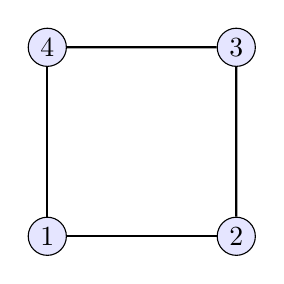
\begin{tikzpicture}[scale=1.2, node distance=2cm, every node/.style={circle, draw, fill=blue!10, inner sep=2pt}]
            \node (v1) at (0,0) {1};
            \node (v2) at (2,0) {2};
            \node (v3) at (2,2) {3};
            \node (v4) at (0,2) {4};
            \draw[thick] (v1) -- (v2);
            \draw[thick] (v2) -- (v3);
            \draw[thick] (v3) -- (v4);
            \draw[thick] (v4) -- (v1);
        \end{tikzpicture}
    \end{center}
    Matriks ketetanggaan $\*A$ untuk graf di atas adalah
    \[
        \*A =
        \begin{pmatrix}
            0 & 1 & 0 & 1 \\
            1 & 0 & 1 & 0 \\
            0 & 1 & 0 & 1 \\
            1 & 0 & 1 & 0
        \end{pmatrix}.
    \]
    Dengan kata lain, matriks derajatnya $\*D = \mathrm{diag}(2,2,2,2)$.
\end{contoh}

\begin{definisi}[\textbf{Graf Laplacian, \citep{chung1997}}]
    Graf Laplacian adalah $\*L=\*D-\*A$. Normalisasi simetris diberikan oleh
    \begin{equation}
        \*L_{\text{sym}} = \*I - \*D^{-1/2}\*A\*D^{-1/2}.
    \end{equation}
\end{definisi}

\noindent Graf Laplacian merepresentasikan struktur graf dan digunakan dalam berbagai algoritma GNN.

\begin{contoh}
    Misalkan graf $\mathcal{G}$ dengan $4$ simpul dan sisi $\mathcal{E} = \{(1,2), (2,3), (3,4), \allowbreak (4,1)\}$ (graf siklus). Matriks ketetanggaannya adalah
    \[
        \*A =
        \begin{pmatrix}
            0 & 1 & 0 & 1 \\
            1 & 0 & 1 & 0 \\
            0 & 1 & 0 & 1 \\
            1 & 0 & 1 & 0
        \end{pmatrix}
    \]
    dan matriks derajatnya adalah
    \[
        \*D = \mathrm{diag}(2,2,2,2).
    \]
    Graf Laplacian-nya dapat dihitung sebagai
    \[
        \*L = \*D - \*A =
        \begin{pmatrix}
            2 & -1 & 0 & -1 \\
            -1 & 2 & -1 & 0 \\
            0 & -1 & 2 & -1 \\
            -1 & 0 & -1 & 2
        \end{pmatrix}.
    \]
    Sehingga, dengan normalisasi simetris didapatkan
    \[
        \*L_{\text{sym}} = \*I - \frac{1}{2}\*A,
    \]
    karena $\*D^{-1/2} = \mathrm{diag}(1/\sqrt{2}, 1/\sqrt{2}, 1/\sqrt{2}, 1/\sqrt{2})$.
\end{contoh}


\begin{teorema}[\textbf{Teorema Spektral Laplacian, \citep{chung1997}}]
    Matriks Laplacian $\*L$ adalah simetris dan positif semidefinit, sehingga dapat didekomposisi dengan dekomposisi nilai eigen sebagai berikut.
    \begin{equation}
        \*L = \*U \bs\Lambda \*U^\top,
    \end{equation}
    dengan $\*U$ ortogonal dan $\bs\Lambda$ diagonal berisi nilai eigen
    $\lambda_1,\dots,\lambda_n \ge 0$. Selalu berlaku $\lambda_1=0$ dengan vektor
    eigen $\*1$.
\end{teorema}

\subsection{Kerangka Penyampaian Pesan pada Jaringan Saraf}

\begin{definisi}[\textbf{\emph{Message Passing Neural Networks} (MPNN), \citep{bronstein2021}}]
    Misalkan graf $\mathcal{G}=(\mathcal{V},\mathcal{E})$ dengan $\mathcal{V}$ adalah himpunan simpul dan $\mathcal{E}$ adalah himpunan sisi. Misalkan pula $\mathcal{N}_u$ adalah ketetanggaan simpul $u \in \mathcal{V}$. Lebih lanjut, misalkan $\bm x_u$ adalah fitur simpul $u$ dan $\bm e_{uv}$ adalah fitur sisi $(u,v) \in \mathcal{E}$. Suatu lapisan MPNN didefinisikan sebagai berikut.
    \begin{equation}
        \bm h_u = \varphi\left(\bm x_u, \bigoplus_{v \in \mathcal{N}_u}\psi(\bm x_u, \bm x_v, \bm e_{uv}),\right)
    \end{equation}
    dengan $\varphi$ dan $\psi$ adalah fungsi yang terdiferensiasi (seperti jaringan saraf) dan $\bigoplus$ adalah operator agregasi yang bersifat komutatif dan asosiatif (seperti penjumlahan atau rata-rata) atau \emph{permutation invariant}.
\end{definisi}

Kerangka MPNN ini sangat fleksibel dan dapat disesuaikan dengan berbagai jenis data graf. Fungsi $\psi$ dapat dirancang untuk menangkap interaksi spesifik antara simpul dan sisi, sedangkan fungsi $\varphi$ dapat berupa jaringan saraf yang kompleks untuk pembaruan fitur. Operator agregasi $\bigoplus$ memastikan bahwa model tetap invariant terhadap permutasi tetangga, yang penting dalam konteks graf. Beberapa arsitektur umum GNN, seperti \emph{Graph Convolutional Networks} (GCN) dan \emph{Graph Attention Networks} (GAT), dapat dianggap sebagai kasus khusus dari kerangka MPNN ini.

\subsection{Arsitektur Umum dalam GNN}

\begin{definisi}[\textbf{Graph Convolutional Networks (GCN), \citep{kipf2017}}]
    GCN mendefinisikan operasi propagasi lapisan ke-$l$ sebagai
    \begin{equation}
        \bm{H}^{(l+1)} = \sigma\!\left(\tilde{\*D}^{-1/2}\tilde{\*A}\tilde{\*D}^{-1/2}\bm{H}^{(l)} \*W^{(l)}\right),
    \end{equation}
    dengan:
    \begin{itemize}
        \item $\tilde{\*A} = \*A + \*I_n$ matriks ketetanggaan dengan \emph{self-loop},
        \item $\tilde{\*D} = \mathrm{diag}(\sum_j \tilde{A}_{ij})$ matriks derajat dari $\tilde{\*A}$,
        \item $\bm{H}^{(l)} \in \mathbb{R}^{n\times d_l}$ representasi simpul pada lapisan $l$,
        \item $\*W^{(l)} \in \mathbb{R}^{d_l \times d_{l+1}}$ bobot terlatih, dan
        \item $\sigma(\cdot)$ fungsi aktivasi non-linear.
    \end{itemize}
    GCN merupakan kasus khusus dari kerangka MPNN dengan:
    \begin{itemize}
        \item Fitur sisi diabaikan ($\bm e_{uv}$ tidak digunakan).
        \item Fungsi pesan $\psi(\bm x_u, \bm x_v, \bm e_{uv}) = \bm x_v$ (hanya mengambil fitur tetangga).
        \item Operator agregasi $\bigoplus$ berupa penjumlahan atau rata-rata tertimbang (melalui normalisasi Laplacian).
        \item Fungsi update $\varphi$ adalah komposisi linear dan aktivasi non-linear: $\varphi(\bm x_u, \mathrm{AGG}) = \sigma(\mathrm{AGG} \cdot \*W)$.
    \end{itemize}
    Secara eksplisit, propagasi GCN dapat ditulis sebagai
    \[
        \bm h_u^{(l+1)} = \sigma\left( \sum_{v \in \mathcal{N}_u \cup \{u\}} \frac{1}{\sqrt{d_u d_v}}\, \bm h_v^{(l)} \*W^{(l)} \right),
    \]
    dengan $d_u$ derajat simpul $u$ dan $\sigma$ fungsi aktivasi. Matriks normalisasi simetris $\tilde{\*D}^{-1/2}\tilde{\*A}\tilde{\*D}^{-1/2}$ merepresentasikan agregasi pesan dari tetangga dengan bobot yang sesuai, sehingga GCN adalah MPNN dengan agregasi rata-rata dan update linear.
\end{definisi}

\begin{definisi}[\textbf{Graph Attention Networks (GAT), \citep{velickovic2018}}]
    GAT mengganti normalisasi derajat dengan mekanisme perhatian.
    Koefisien perhatian untuk sisi $(i,j)$ adalah
    \begin{equation}
        \alpha_{ij} = \frac{\exp\!\left(\mathrm{LeakyReLU}\!\big(\bm{a}^\top [\*W\bm{h}_i \,\|\, \*W\bm{h}_j]\big)\right)}{\sum_{k \in \mathcal{N}(i)} \exp\!\left(\mathrm{LeakyReLU}\!\big(\*a^\top [\*W\bm{h}_i \,\|\, \*W\bm{h}_k]\big)\right)},
    \end{equation}
    dengan:
    \begin{itemize}
        \item $\bm{h}_i \in \mathbb{R}^{d}$ vektor fitur simpul $i$,
        \item $\*W$ bobot transformasi linear,
        \item $\bm{a} \in \mathbb{R}^{2d'}$ vektor bobot perhatian, dan
        \item $\|$ operator konkatenasi.
    \end{itemize}
    Pembaruan fitur simpul adalah
    \begin{equation}
        \*h_i' = \sigma\!\left(\sum_{j\in\mathcal{N}(i)} \alpha_{ij}\*W\bm{h}_j\right).
    \end{equation}
    GAT merupakan kasus khusus dari kerangka MPNN dengan spesifikasi berikut.
    \begin{itemize}
        \item Fitur sisi $\bm{e}_{uv}$ tidak digunakan (atau dapat diabaikan).
        \item Fungsi pesan $\psi(\bm{x}_u, \bm{x}_v, \bm{e}_{uv}) = \*W\bm{x}_v$ (transformasi linear fitur tetangga).
        \item Operator agregasi $\bigoplus$ berupa penjumlahan tertimbang, dengan bobot agregasi $\alpha_{uv}$ diperoleh dari mekanisme perhatian (\emph{attention}) yang bersifat permutation invariant.
        \item Fungsi update $\varphi$ adalah komposisi linear dan aktivasi non-linear: $\varphi(\bm{x}_u, \mathrm{AGG}) = \sigma(\mathrm{AGG})$.
    \end{itemize}
    Secara formal, pembaruan fitur simpul $u$ pada GAT dapat ditulis dalam notasi MPNN sebagai
    \begin{equation}
        \bm{h}_u' = \sigma\left(\sum_{v \in \mathcal{N}_u} \alpha_{uv} \psi(\bm{x}_u, \bm{x}_v, \bm{e}_{uv})\right)
        = \sigma\left(\sum_{v \in \mathcal{N}_u} \alpha_{uv} \*W\bm{x}_v\right),
    \end{equation}
    dengan $\alpha_{uv}$ adalah skor perhatian yang bergantung pada fitur $\bm{x}_u$ dan $\bm{x}_v$ melalui fungsi $\mathrm{LeakyReLU}(\*a^\top [\*W\bm{x}_u \,\|\, \*W\bm{x}_v])$ dan normalisasi softmax. Dengan demikian, GAT adalah MPNN dengan agregasi penjumlahan tertimbang dan fungsi pesan linear dengan bobot agregasi ditentukan secara adaptif oleh mekanisme perhatian.
\end{definisi}

\begin{definisi}[\textbf{GraphSAGE, \citep{hamilton2017}}]
    GraphSAGE atau \emph{Graph Sample and Aggregation} mendefinisikan pembaruan simpul $i$ sebagai
    \begin{equation}
        \bm h_i^{(l+1)} = \sigma\!\left(\bm W^{(l)} \cdot \mathrm{AGGREGATE}\left(\{\bm h_i^{(l)}\}\cup \{\bm h_j^{(l)}: j\in\mathcal{N}(i)\}\right)\right),
    \end{equation}
    dengan $\mathrm{AGGREGATE}$ fungsi agregasi non-linear yang bisa berupa
    \emph{mean}, \emph{max-pooling}, atau LSTM.
\end{definisi}

\subsection{Kekuatan Representasi GNN}

\begin{definisi}[\textbf{Isomorfisme Graf}]
    Dua graf $\mathcal{G}_1=(\mathcal{V}_1,\mathcal{E}_1)$ dan $\mathcal{G}_2=(\mathcal{V}_2,\mathcal{E}_2)$ disebut isomorfik jika terdapat bijeksi $\pi:\mathcal{V}_1 \to \mathcal{V}_2$ sehingga
    \begin{equation}
        (i,j)\in\mathcal{E}_1 \iff (\pi(i),\pi(j))\in\mathcal{E}_2.
    \end{equation}
    Sebuah fungsi $f$ dikatakan \emph{invarian terhadap isomorfisme graf} jika
    $f(\mathcal{G}_1)=f(\mathcal{G}_2)$ untuk setiap graf isomorfik
    $\mathcal{G}_1\cong \mathcal{G}_2$.
\end{definisi}

\begin{contoh}
    Misalkan $\mathcal{G}_1$ adalah graf dengan simpul $\{1,2,3\}$ dan sisi $\{(1,2), \allowbreak (2,3),(3,1)\}$ (graf segitiga). Ambil $\mathcal{G}_2$ dengan simpul $\{a,b,c\}$ dan sisi $\{(a,b),\allowbreak(b,c),(c,a)\}$. Bijeksi $\pi$ dapat dipilih misal $\pi(1)=a$, $\pi(2)=b$, $\pi(3)=c$. Maka $\mathcal{G}_1$ dan $\mathcal{G}_2$ isomorfik.

    Sebagai contoh fungsi invarian, jumlah simpul $|\mathcal{V}|$ dan jumlah sisi $|\mathcal{E}|$ adalah invarian terhadap isomorfisme graf. Demikian juga, spektrum Laplacian graf $\*L$ adalah invarian terhadap isomorfisme.

    \begin{figure}[H]
        \centering
        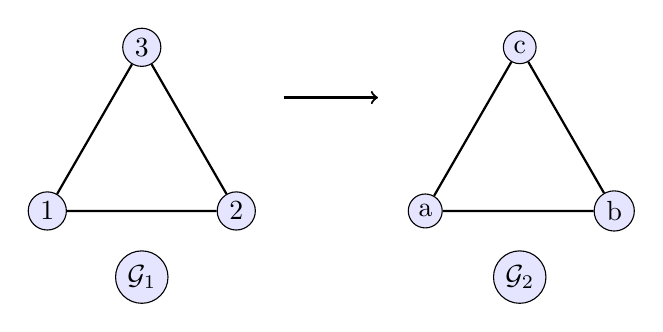
\begin{tikzpicture}[scale=1.2, node distance=2cm, every node/.style={circle, draw, fill=blue!10, inner sep=2pt}]
            % Graph G1
            \node (v1) at (0,0) {1};
            \node (v2) at (2,0) {2};
            \node (v3) at (1,1.732) {3};
            \draw[thick] (v1) -- (v2) -- (v3) -- (v1);
            \node at (1,-0.7) {$\mathcal{G}_1$};

            % Arrow for isomorphism
            \draw[->, thick] (2.5,1.2) -- (3.5,1.2);
            \node (a) at (4,0) {a};
            \node (b) at (6,0) {b};
            \node (c) at (5,1.732) {c};
            \draw[thick] (a) -- (b) -- (c) -- (a);
            \node at (5,-0.7) {$\mathcal{G}_2$};
        \end{tikzpicture}
        \caption{Ilustrasi dua graf isomorfik, yaitu $\mathcal{G}_1$ dan $\mathcal{G}_2$ memiliki struktur yang sama walaupun label simpul berbeda. (Sumber: Dokumen penulis)}
    \end{figure}
\end{contoh}

\begin{definisi}[\textbf{Tes Weisfeiler--Lehman (WL) Satu Dimensi}]
    Algoritma WL satu dimensi, juga dikenal sebagai \emph{color refinement}, merupakan prosedur iteratif untuk membedakan graf berdasarkan struktur lokal simpul. Pada setiap iterasi, label simpul $h_i^{(t)}$ diperbarui dengan cara:
    \begin{equation}
        h_i^{(t+1)} = \mathrm{HASH}\!\left(h_i^{(t)}, \{h_j^{(t)} : j \in \mathcal{N}(i)\}\right),
    \end{equation}
    dimulai dari label awal $h_i^{(0)}$. Dua graf dikatakan dapat dibedakan oleh tes WL jika multiset label akhirnya berbeda. Dalam konteks pembelajaran mesin, tes WL memberikan kerangka formal untuk mengukur kemampuan model, seperti GNN, dalam membedakan struktur graf yang berbeda melalui proses agregasi informasi dari tetangga.
\end{definisi}

Fungsi $\mathrm{HASH}$ pada algoritma WL berperan sebagai pemetaan yang menggabungkan label simpul saat ini dengan label-label tetangganya menjadi label baru yang unik. Intuisi utamanya adalah memastikan bahwa jika dua simpul memiliki lingkungan yang berbeda, hasil $\mathrm{HASH}$ juga berbeda. Dalam implementasi praktis, $\mathrm{HASH}$ dapat berupa fungsi injektif seperti pengkodean \emph{string}, \emph{concatenation}, atau fungsi neural yang mampu membedakan multiset masukan secara efektif.

\begin{teorema}[\textbf{Keterbatasan GNN Berbasis Agregasi, \citep{xu2019}}]
    GNN berbasis agregasi dengan pembaruan umum
    \begin{equation}
        h_i^{(l+1)} = \varphi\!\left( W^{(l)} \cdot \mathrm{AGGREGATE}\big(\{h_i^{(l)}\}\cup\{h_j^{(l)}: j\in \mathcal{N}(i)\}\big)\right)
    \end{equation}
    tidak lebih kuat daripada tes WL satu dimensi dalam membedakan graf yang tidak isomorfik. Artinya, kemampuan GNN untuk membedakan struktur graf dibatasi oleh kekuatan agregasi lokal yang serupa dengan tes WL.
\end{teorema}

\begin{teorema}[\textbf{Hubungan dengan Tes WL, \citep{xu2019}}]
    Jika fungsi agregasi $\mathrm{AGGREGATE}$ bersifat injektif terhadap multiset, maka GNN memiliki kekuatan representasi setara dengan tes WL satu dimensi. Dengan kata lain, GNN dapat membedakan graf sejauh tes WL mampu membedakannya, asalkan agregasi dan pembaruan fitur dilakukan secara unik untuk setiap lingkungan simpul.
\end{teorema}

\section{Inferensi Kausal dengan Pembelajaran Mesin Ganda}


% \section{Pembelajaran Representasi}

% Pembelajaran representasi (\textit{representation learning}) bertujuan mempelajari transformasi dari data mentah ke bentuk fitur yang lebih sesuai untuk tugas pembelajaran. Secara formal, algoritma pembelajaran representasi mencari transformasi $\phi$ yang memetakan data observasi $x$ ke representasi $h = \phi(x)$, sehingga prediktor sederhana $f$ dapat memodelkan target $y$ dari $h$ secara efisien.

% Pembelajaran representasi merupakan cabang pembelajaran mesin yang berfokus pada pembentukan representasi data yang memudahkan ekstraksi informasi penting untuk klasifikasi atau prediksi. Pendekatan ini menggantikan rekayasa fitur manual dengan proses otomatis yang mempelajari struktur intrinsik data. Dengan representasi yang baik, model dapat menangkap faktor penyebab utama data dan mengabaikan variasi yang tidak relevan terhadap tugas.

% Tujuan utama pembelajaran representasi adalah memisahkan faktor-faktor variasi yang mendasari data dan merepresentasikannya agar lebih mudah dipisahkan untuk tugas prediksi berikutnya. Representasi yang baik tidak hanya memampatkan informasi, tetapi juga mengorganisasi struktur data sehingga faktor penting dapat diakses secara eksplisit oleh model.

% Dalam pembelajaran mendalam, pembelajaran representasi memegang peran sentral karena memungkinkan sistem secara otomatis menemukan representasi yang diperlukan untuk deteksi fitur atau klasifikasi langsung dari data mentah. Proses ini menghasilkan vektor representasi $\phi(x)$ yang memuat informasi relevan dengan tugas, sekaligus menekan dimensi dan variasi yang tidak diperlukan. Representasi yang baik memudahkan fungsi $f$ sederhana (misalnya regresi linear atau \emph{softmax}) untuk mencapai kinerja tinggi tanpa rekayasa fitur tambahan.

% Secara ringkas, pembelajaran representasi merupakan kerangka umum untuk
% \begin{enumerate}[label=(\alph*)]
%     \item mempelajari pemetaan $\phi$ dari data mentah $x$ ke ruang fitur laten $h$,
%     \item menstrukturkan ulang informasi agar faktor variasi yang relevan menjadi terpisah, dan
%     \item memfasilitasi pembelajaran fungsi prediksi sederhana $f$ di ruang laten.
% \end{enumerate}
% Pendekatan ini menjadi dasar konseptual bagi jaringan saraf tiruan modern dan seluruh keluarga model pembelajaran mendalam.

% \begin{definisi}[\textbf{Sifat Representasi yang Baik}]
%     Menurut \citet{goodfellow2016}, representasi yang baik adalah transformasi $\phi(x)$ dari data mentah $x$ ke ruang laten yang memenuhi sifat-sifat berikut.
%     \begin{enumerate}[label=(\alph*)]
%         \item Invariansi, yaitu Representasi tidak berubah terhadap variasi tak relevan pada input, seperti translasi, rotasi, atau gangguan acak yang tidak memengaruhi makna semantik.
%         \item \emph{Disentanglement}, yaitu Setiap dimensi dalam ruang laten memuat faktor penyebab utama yang terpisah, sehingga informasi penting tidak tercampur.
%         \item Efisiensi, yaitu Representasi bersifat jarang (sparse) atau berdimensi rendah, sehingga memudahkan penyimpanan, pemrosesan, dan generalisasi.
%         \item Transferabilitas, yaitu Representasi dapat digunakan ulang untuk berbagai tugas berbeda tanpa pelatihan ulang yang ekstensif.
%     \end{enumerate}
% \end{definisi}

% Suatu transformasi $\phi$ dikatakan menghasilkan representasi yang baik jika:
% \begin{enumerate}[label=(\alph*)]
%     \item memisahkan faktor-faktor variasi utama dalam data sehingga fungsi target $f$ dapat dipelajari secara sederhana di ruang laten,
%     \item membuat prediksi menjadi lebih mudah dan stabil terhadap perubahan kecil pada input yang tidak relevan, dan
%     \item memungkinkan generalisasi dan transfer ke tugas baru dengan sedikit data berlabel.
% \end{enumerate}

% \subsection{Landasan Teoretis Representasi}

% \begin{definisi}[\textbf{Invariansi dan Equivariansi, \citealp{goodfellow2016}}]
%     Suatu representasi $\phi:\mathcal{X}\to\mathcal{Z}$ dikatakan \emph{invarian} terhadap grup transformasi $G$ jika memenuhi
%     \begin{equation}
%         \phi(g\cdot x)=\phi(x), \qquad \forall g\in G,\ x\in\mathcal{X}.
%     \end{equation}
%     Sebaliknya, $\phi$ disebut \emph{equivariant} terhadap $G$
%     jika terdapat aksi linear $T_g$ pada $\mathcal{Z}$ sehingga
%     \begin{equation}
%         \phi(g\cdot x)=T_g\,\phi(x).
%     \end{equation}
% \end{definisi}

% Representasi yang baik seharusnya invarian terhadap faktor-faktor yang tidak memengaruhi konsep target, seperti translasi kecil pada citra atau perubahan kondisi pencahayaan. Invariansi menjadi kunci agar model tidak sensitif terhadap variasi yang tidak bermakna secara semantik.

% \begin{contoh}
%     Pada klasifikasi digit MNIST, translasi kecil pada posisi angka
%     tidak boleh mengubah representasi laten digit tersebut.
%     Dalam jaringan konvolusional, fungsi $\phi$ dirancang
%     agar bersifat \emph{equivariant} terhadap translasi,
%     sehingga pergeseran lokasi pada ruang input
%     hanya memindahkan posisi aktivasi tanpa mengubah nilainya.
% \end{contoh}

% \begin{definisi}[\textbf{Hipotesis Manifold, \citealp{bengio2013}}]
%     Misalkan data $x\in\mathbb{R}^D$ terdistribusi di sekitar Manifold berdimensi rendah
%     $\mathcal{M}\subset\mathbb{R}^D$.
%     Hipotesis Manifold menyatakan bahwa terdapat pemetaan kontinu
%     \begin{equation}
%         \phi:\mathbb{R}^D\to\mathbb{R}^d, \quad d\ll D,
%     \end{equation}
%     yang memparametrisasi koordinat intrinsik Manifold $\mathcal{M}$,
%     sehingga setiap titik $x$ dapat direpresentasikan oleh koordinat laten $\phi(x)$.
% \end{definisi}

% Manifold adalah konsep matematis yang merepresentasikan himpunan titik-titik dalam ruang berdimensi tinggi yang secara lokal menyerupai ruang Euclidean berdimensi lebih rendah. Dalam konteks pembelajaran mesin, Manifold digunakan untuk menjelaskan bahwa data berdimensi tinggi sebenarnya terletak pada atau di sekitar permukaan berdimensi rendah di dalam ruang fitur aslinya. Misalnya, meskipun gambar digital memiliki ribuan piksel (dimensi tinggi), variasi utama seperti pose, pencahayaan, atau ekspresi wajah hanya membentuk beberapa derajat kebebasan (dimensi rendah).

% Hipotesis Manifold menyatakan bahwa data nyata tidak tersebar secara acak di seluruh ruang berdimensi tinggi, melainkan terkonsentrasi di sekitar Manifold berdimensi rendah yang dibentuk oleh faktor-faktor variasi utama. Oleh karena itu, pembelajaran representasi yang efektif bertujuan menemukan koordinat intrinsik Manifold ini, sehingga model dapat memisahkan faktor penyebab utama dan mengabaikan variasi yang tidak relevan. Pendekatan ini mendasari banyak metode modern, seperti \emph{autoencoder}, pembelajaran berbasis graf, dan pembelajaran semi-terawasi, yang semuanya memanfaatkan struktur Manifold untuk meningkatkan generalisasi dan efisiensi model.

% \begin{teorema}[\textbf{Hipotesis Manifold dan Invariansi, \citealp{goodfellow2016}}]
%     Jika data $x\in\mathbb{R}^D$ berada pada Manifold berdimensi rendah $\mathcal{M}$,
%     dan grup transformasi $G$ bertindak pada $\mathcal{M}$,
%     maka terdapat representasi $\phi$ yang \emph{equivariant} terhadap aksi $G$
%     yang memproyeksikan $\mathcal{M}$ ke koordinat intrinsiknya.  
%     Secara khusus, $\phi(g\!\cdot\!x)=T_g\,\phi(x)$
%     dengan $T_g$ aksi linear pada ruang laten.
% \end{teorema}

% \begin{contoh}
%     Dalam pengenalan wajah, meskipun setiap gambar memiliki ribuan piksel,
%     variasi utamanya (arah pandangan, pencahayaan, ekspresi)
%     dapat dijelaskan oleh beberapa koordinat laten berdimensi rendah.
%     Fungsi $\phi$ bertugas memetakan gambar beresolusi tinggi tersebut
%     ke ruang laten yang memuat koordinat intrinsik wajah yang sama
%     terlepas dari variasi pose dan pencahayaan.
% \end{contoh}

% \section{Pembelajaran Semi-Terawasi}

% Pembelajaran semi-terawasi (\emph{semi-supervised learning}, SSL) adalah paradigma pembelajaran mesin yang memanfaatkan kombinasi data berlabel dalam jumlah kecil dan data tak berlabel dalam jumlah besar untuk meningkatkan kinerja model. Pendekatan ini sangat relevan dalam konteks praktis karena pelabelan data seringkali memerlukan biaya tinggi, waktu lama, dan keahlian khusus, sementara data tak berlabel dapat diperoleh dengan mudah dan murah. Dengan memanfaatkan struktur intrinsik dari data tak berlabel, SSL dapat menghasilkan model dengan generalisasi lebih baik dibandingkan pembelajaran terawasi murni yang hanya mengandalkan data berlabel terbatas.

% \subsection{Kerangka Dasar}

% Dalam banyak aplikasi pembelajaran mesin, memperoleh label memerlukan intervensi manusia yang mahal atau proses eksperimen yang memakan waktu. Sebagai contoh, dalam klasifikasi dokumen teks, pelabelan manual ribuan artikel memerlukan waktu dan keahlian domain yang signifikan. Sebaliknya, mengumpulkan dokumen tak berlabel dari internet sangat mudah. SSL berupaya menjembatani kesenjangan ini dengan mengekstraksi informasi dari distribusi data tak berlabel untuk memperkaya proses pembelajaran.

% \begin{definisi}[\textbf{Kerangka Pembelajaran Semi-Terawasi, \citep{chapelle2006}}]
% Diberikan himpunan data berlabel $\mathcal{D}_\ell = \{(\*x_i, y_i)\}_{i=1}^{\ell}$ dan himpunan data tak berlabel $\mathcal{D}_u = \{\*x_j\}_{j=\ell+1}^{n}$, dengan $\*x \in \mathcal{X} \subseteq \mathbb{R}^p$ adalah vektor fitur dan $y \in \mathcal{Y}$ adalah label (diskret untuk klasifikasi atau kontinu untuk regresi). Dalam konteks SSL, jumlah data tak berlabel umumnya jauh lebih besar daripada data berlabel, yaitu $u = n - \ell \gg \ell$.

% Tujuan SSL adalah mempelajari fungsi prediksi $f: \mathcal{X} \to \mathcal{Y}$ yang memanfaatkan informasi dari kedua himpunan data. Formulasi umum masalah optimasi SSL adalah
% \begin{equation}
% \min_{f \in \mathcal{F}} \quad \underbrace{\frac{1}{\ell} \sum_{i=1}^{\ell} \mathcal{L}(f(\*x_i), y_i)}_{\text{kerugian terawasi}} + \lambda \underbrace{\mathcal{R}(f; \mathcal{D}_u)}_{\text{regularisasi dari data tak berlabel}},
% \end{equation}
% dengan $\mathcal{F}$ adalah kelas fungsi hipotesis, $\mathcal{L}$ adalah fungsi kerugian terawasi, $\mathcal{R}$ adalah term regularisasi yang mengekstrak struktur dari data tak berlabel, dan $\lambda > 0$ adalah parameter yang mengatur trade-off antara kedua komponen tersebut.
% \end{definisi}

% \begin{contoh}
% Dalam klasifikasi dokumen, misalkan terdapat 100 dokumen berlabel tentang topik \emph{politik} dan \emph{olahraga}, serta 10{,}000 dokumen tak berlabel. SSL dapat memanfaatkan kemiripan antar dokumen tak berlabel untuk membentuk klaster yang koheren, sehingga model dapat belajar bahwa dokumen dengan kata-kata mirip cenderung memiliki label yang sama, meskipun label eksplisit tidak tersedia untuk sebagian besar dokumen.
% \end{contoh}


% Menurut \citet{chapelle2006}, SSL dapat dikategorikan menjadi dua kerangka sebagai berikut.
% \begin{enumerate}[label=(\alph*)]
%     \item Pembelajaran induktif, yaitu model mempelajari fungsi $f:\mathcal{X}\to\mathcal{Y}$ 
%     yang dapat digeneralisasikan ke data baru di luar himpunan pelatihan.
%     Ini adalah pendekatan umum yang digunakan dalam kebanyakan aplikasi modern.
%     \item Pembelajaran transduktif, yang tujuannya hanya untuk memprediksi label dari sejumlah data tak berlabel tertentu
%     yang telah diketahui selama pelatihan, tanpa menggeneralisasi ke sampel baru.
% \end{enumerate}
% \citet{grandvalet2005semi} menambahkan bahwa SSL dapat dilihat
% sebagai jembatan antara pembelajaran induktif dan transduktif,
% karena ia memanfaatkan informasi struktur global dari semua data
% untuk memperbaiki estimasi pada titik tak berlabel yang diamati.


% \subsection{Asumsi Fundamental dalam Pembelajaran Semi-Terawasi}

% Keberhasilan SSL bergantung pada asumsi-asumsi tertentu tentang struktur data yang menghubungkan distribusi fitur $p(\*x)$ dengan distribusi label kondisional $p(y \mid \*x)$. Tanpa asumsi ini, data tak berlabel tidak memberikan informasi tambahan yang berguna \citep{chapelle2006}.

% \begin{definisi}[\textbf{Asumsi Kehalusan (\emph{Smoothness Assumption}), \citep{chapelle2006}}]
% Jika dua titik $\*x_1, \*x_2 \in \mathcal{X}$ berada dalam daerah berdensitas tinggi dan berdekatan satu sama lain, maka label yang bersesuaian $y_1$ dan $y_2$ cenderung sama. Secara formal, fungsi $f$ yang baik harus bersifat halus pada daerah berdensitas tinggi, yaitu
% \begin{equation}
% \|\*x_i - \*x_j\|^2 \text{ kecil} \implies |f(\*x_i) - f(\*x_j)| \text{ kecil},
% \end{equation}
% untuk $\*x_i, \*x_j$ yang terletak pada daerah dengan $p(\*x)$ tinggi.
% \end{definisi}

% \begin{contoh}
% Dalam pengenalan gambar wajah, dua gambar wajah yang hanya berbeda sedikit dalam pencahayaan atau rotasi kecil (jarak Euclidean kecil dalam ruang piksel) seharusnya memiliki identitas yang sama. Asumsi kehalusan menyatakan bahwa fungsi klasifikasi tidak boleh berubah drastis pada perubahan kecil seperti ini.
% \end{contoh}

% \begin{definisi}[\textbf{Asumsi Klaster (\emph{Cluster Assumption}), \citep{chapelle2006}}]
% Data cenderung membentuk klaster-klaster yang terpisah, dan titik-titik dalam klaster yang sama cenderung memiliki label yang sama. Batas keputusan yang baik seharusnya melewati daerah berdensitas rendah, bukan memotong klaster.

% Secara matematis, jika terdapat jalur $\gamma: [0,1] \to \mathcal{X}$ yang menghubungkan $\*x_i$ dengan $\*x_j$ sedemikian sehingga $p(\gamma(t))$ tinggi untuk semua $t \in [0,1]$, maka $f(\*x_i) \approx f(\*x_j)$.
% \end{definisi}

% \begin{contoh}
% Misalkan data terdiri dari dua klaster Gaussian yang terpisah jauh. Jika beberapa titik dari klaster pertama diberi label ``positif'' dan beberapa titik dari klaster kedua diberi label ``negatif'', maka batas keputusan optimal seharusnya berada di antara kedua klaster (daerah berdensitas rendah), bukan memotong salah satu klaster.
% \end{contoh}

% \begin{definisi}[\textbf{Asumsi Manifold (\emph{Manifold Assumption}), \citep{chapelle2006}}]
% Data berdimensi tinggi $\*x \in \mathbb{R}^p$ sebenarnya terletak pada atau dekat dengan Manifold berdimensi rendah $\mathcal{M} \subset \mathbb{R}^p$. Fungsi $f$ yang baik seharusnya bervariasi secara halus sepanjang struktur geometri Manifold $\mathcal{M}$ ini, bukan sepanjang ruang ambien $\mathbb{R}^p$.

% Asumsi ini memotivasi penggunaan regularisasi berbasis geometri, seperti Laplasian graf, untuk menekan variasi $f$ sepanjang Manifold yang didefinisikan oleh data.
% \end{definisi}

% \begin{contoh}
% Dalam \emph{dataset} gambar wajah, meskipun setiap gambar memiliki ribuan piksel (dimensi tinggi), variasi sesungguhnya (pose, ekspresi, pencahayaan) berada pada Manifold berdimensi jauh lebih rendah. SSL yang memanfaatkan asumsi Manifold akan mempelajari representasi yang menghormati struktur geometri intrinsik ini.
% \end{contoh}

% \subsection{Fungsi Kerugian untuk Pembelajaran Semi-Terawasi}

% Desain fungsi kerugian yang tepat merupakan aspek krusial dalam SSL karena menentukan bagaimana informasi dari data tak berlabel dimanfaatkan untuk memperbaiki model. Berbeda dengan pembelajaran terawasi yang hanya menggunakan kerugian pada data berlabel, SSL memerlukan komponen tambahan yang mengekstraksi informasi dari data tak berlabel \citep{chapelle2006}.

% \begin{definisi}[\textbf{Struktur Umum Fungsi Kerugian SSL, \citep{chapelle2006}}]
% Fungsi kerugian total dalam SSL dapat didekomposisi menjadi tiga komponen:
% \begin{equation}
% \mathcal{L}_{\text{total}} = \mathcal{L}_{\text{supervised}} + \lambda_u \mathcal{L}_{\text{unsupervised}} + \lambda_r \mathcal{R}(\theta),
% \end{equation}
% dengan:
% \begin{itemize}
%     \item $\mathcal{L}_{\text{supervised}} = \frac{1}{\ell} \sum_{i=1}^{\ell} \ell(f_\theta(\*x_i), y_i)$ adalah kerugian terawasi standar pada data berlabel,
%     \item $\mathcal{L}_{\text{unsupervised}}$ adalah kerugian yang mengekstrak informasi dari data tak berlabel,
%     \item $\mathcal{R}(\theta)$ adalah regularisasi pada parameter model,
%     \item $\lambda_u, \lambda_r > 0$ adalah hyperparameter yang mengontrol kontribusi masing-masing komponen.
% \end{itemize}
% \end{definisi}

% Komponen kunci yang membedakan berbagai metode SSL adalah desain $\mathcal{L}_{\text{unsupervised}}$. Beberapa pendekatan utama akan dijelaskan berikut ini.

% Salah satu prinsip fundamental untuk memanfaatkan data tak berlabel adalah \emph{entropy minimization}, yang didasarkan pada intuisi bahwa model yang baik seharusnya membuat prediksi yang percaya diri (\emph{low entropy}) pada semua data, termasuk data tak berlabel \citep{grandvalet2005semi}.

% \begin{definisi}[\textbf{Kerugian Entropi untuk SSL, \citep{grandvalet2005semi}}]
% Untuk klasifikasi multi-kelas dengan $C$ kelas, diberikan model probabilistik yang menghasilkan distribusi prediksi $\hat{\*p}(y \mid \*x) = f_\theta(\*x) \in \Delta^{C-1}$ (simplex probabilitas $C$-dimensi). Entropi kondisional dari prediksi adalah
% \begin{equation}
% H(y \mid \*x; \theta) = -\sum_{c=1}^{C} \hat{p}_c(\*x; \theta) \log \hat{p}_c(\*x; \theta),
% \end{equation}
% dengan $\hat{p}_c(\*x; \theta)$ adalah probabilitas prediksi untuk kelas $c$.

% Fungsi kerugian minimisasi entropi untuk data tak berlabel didefinisikan sebagai rata-rata entropi prediksi:
% \begin{equation}
% \mathcal{L}_{\text{entropy}} = \frac{1}{u} \sum_{j=\ell+1}^{n} H(y \mid \*x_j; \theta) = -\frac{1}{u} \sum_{j=\ell+1}^{n} \sum_{c=1}^{C} \hat{p}_c(\*x_j; \theta) \log \hat{p}_c(\*x_j; \theta).
% \end{equation}
% Meminimalkan $\mathcal{L}_{\text{entropy}}$ mendorong model untuk membuat prediksi yang lebih percaya diri (puncak distribusi lebih tajam) pada data tak berlabel.
% \end{definisi}

% \begin{contoh}
% Untuk klasifikasi biner, misalkan model memprediksi probabilitas kelas positif $\hat{p}(\*x) = 0.5$ untuk suatu titik tak berlabel. Entropi prediksi adalah
% \[
% H = -[0.5 \log 0.5 + 0.5 \log 0.5] = -\log 0.5 \approx 0.693 \text{ (maksimum)}.
% \]
% Sebaliknya, jika model percaya diri dengan $\hat{p}(\*x) = 0.95$, maka
% \[
% H = -[0.95 \log 0.95 + 0.05 \log 0.05] \approx 0.198 \text{ (rendah)}.
% \]
% Minimisasi entropi mendorong model menuju prediksi percaya diri seperti kasus kedua.
% \end{contoh}

% Pendekatan lain yang populer adalah \emph{consistency regularization}, yang didasarkan pada prinsip bahwa prediksi model seharusnya konsisten terhadap perturbasi kecil pada input atau model itu sendiri.

% \begin{definisi}[\textbf{Kerugian Konsistensi, \citep{chapelle2006}}]
% Untuk augmentasi atau perturbasi $\mathcal{T}$ (misalnya, noise Gaussian, dropout, augmentasi data), kerugian konsistensi didefinisikan sebagai
% \begin{equation}
% \mathcal{L}_{\text{consistency}} = \frac{1}{u} \sum_{j=\ell+1}^{n} \mathbb{E}_{\tau \sim \mathcal{T}} \big[\|\hat{\*p}(\tau(\bm{x}_j); \theta) - \hat{\*p}(\bm{x}_j; \theta)\|^2\big],
% \end{equation}
% atau dalam bentuk praktis menggunakan sampling:
% \begin{equation}
% \mathcal{L}_{\text{consistency}} = \frac{1}{u} \sum_{j=\ell+1}^{n} \|\hat{\*p}(\tau(\bm{x}_j); \theta) - \hat{\*p}(\bm{x}_j; \theta)\|^2.
% \end{equation}
% Kerugian ini mendorong model untuk menghasilkan prediksi yang sama untuk input yang telah diperturbasi dan input asli.
% \end{definisi}

% \begin{contoh}
% Dalam klasifikasi gambar, augmentasi $\tau$ dapat berupa rotasi kecil, translasi, atau perubahan brightness. Untuk gambar wajah $\bm{x}_j$, jika model memprediksi identitas ``Alice'' dengan probabilitas 0.9, maka setelah rotasi 5 derajat $\tau(\bm{x}_j)$, model seharusnya tetap memprediksi ``Alice'' dengan probabilitas mendekati 0.9. Kerugian konsistensi menghukum deviasi antara kedua prediksi ini.
% \end{contoh}

% Teknik yang lebih sederhana namun efektif adalah \emph{pseudo-labeling}, di mana model digunakan untuk membuat label sementara untuk data tak berlabel, yang kemudian diperlakukan sebagai label sebenarnya dalam iterasi pelatihan berikutnya.

% \begin{definisi}[\textbf{Kerugian Pseudo-Labeling, \citep{chapelle2006}}]
% Untuk setiap titik tak berlabel $\*x_j$, definisikan label seementara sebagai prediksi kelas dengan probabilitas tertinggi:
% \begin{equation}
% \tilde{y}_j = \arg\max_{c \in \{1, \ldots, C\}} \hat{p}_c(\*x_j; \theta).
% \end{equation}
% Kerugian pseudo-labeling adalah:
% \begin{equation}
% \mathcal{L}_{\text{pseudo}} = \frac{1}{u} \sum_{j=\ell+1}^{n} \ell(f_\theta(\*x_j), \tilde{y}_j),
% \end{equation}
% dengan $\ell$ adalah fungsi kerugian standar (misalnya, cross-entropy).
% \end{definisi}

% \begin{contoh}
% Misalkan model memprediksi distribusi probabilitas $[0.05, 0.15, 0.80]$ untuk tiga kelas pada titik tak berlabel $\*x_j$. Pseudo-label adalah $\tilde{y}_j = 3$ (kelas ketiga). Pada iterasi pelatihan berikutnya, titik $\*x_j$ dengan pseudo-label 3 ditambahkan ke set pelatihan dan diperlakukan seolah-olah labelnya adalah 3.
% \end{contoh}

% Untuk data yang dapat direpresentasikan sebagai graf (atau ketika graf kemiripan dapat dikonstruksi), regularisasi berbasis Laplasian graf menyediakan cara alami untuk mengimplementasikan asumsi kehalusan.

% \begin{definisi}[\textbf{Regularisasi Graf Laplacian, \citep{chapelle2006}}]
% Diberikan graf kemiripan dengan matriks bobot $\*W$ dan Laplasian $\*L = \*D - \*W$, regularisasi graf untuk fungsi $f$ didefinisikan sebagai
% \begin{equation}
% \mathcal{R}_{\text{graph}}(f) = \frac{1}{2} \sum_{i,j=1}^{n} w_{ij} \|f(\*x_i) - f(\*x_j)\|^2 = \*f^\top \*L \*f,
% \end{equation}
% dengan $\*f = (f(\bm{x}_1), \ldots, f(\*x_n))^\top$.

% Untuk model \emph{neural} yang menghasilkan representasi laten $\bm{h}_i = \phi_\theta(\*x_i)$, regularisasi graf dapat diterapkan pada representasi:
% \begin{equation}
% \mathcal{L}_{\text{graph}} = \frac{1}{2} \sum_{i,j=1}^{n} w_{ij} \|\bm{}_i - \bm{h}_j\|^2.
% \end{equation}
% \end{definisi}

% \begin{contoh}
% Untuk \emph{dataset} dengan 5 titik dan graf kemiripan berbentuk jalur linear $1 - 2 - 3 - 4 - 5$ dengan bobot seragam $w_{ij} = 1$, jika representasi laten adalah $\bm{h} = [0, 0.2, 0.4, 0.6, 1]^\top$, maka
% \begin{align*}
% \mathcal{L}_{\text{graph}} &= \frac{1}{2} [|0 - 0.2|^2 + |0.2 - 0.4|^2 + |0.4 - 0.6|^2 + |0.6 - 1|^2] \\
% &= \frac{1}{2} [0.04 + 0.04 + 0.04 + 0.16] = 0.14.
% \end{align*}
% Regularisasi ini mendorong representasi simpul yang berdekatan dalam graf untuk memiliki nilai yang mirip.
% \end{contoh}
